% Options for packages loaded elsewhere
\PassOptionsToPackage{unicode}{hyperref}
\PassOptionsToPackage{hyphens}{url}
%
\documentclass[
]{article}
\usepackage{lmodern}
\usepackage{amssymb,amsmath}
\usepackage{ifxetex,ifluatex}
\ifnum 0\ifxetex 1\fi\ifluatex 1\fi=0 % if pdftex
  \usepackage[T1]{fontenc}
  \usepackage[utf8]{inputenc}
  \usepackage{textcomp} % provide euro and other symbols
\else % if luatex or xetex
  \usepackage{unicode-math}
  \defaultfontfeatures{Scale=MatchLowercase}
  \defaultfontfeatures[\rmfamily]{Ligatures=TeX,Scale=1}
\fi
% Use upquote if available, for straight quotes in verbatim environments
\IfFileExists{upquote.sty}{\usepackage{upquote}}{}
\IfFileExists{microtype.sty}{% use microtype if available
  \usepackage[]{microtype}
  \UseMicrotypeSet[protrusion]{basicmath} % disable protrusion for tt fonts
}{}
\makeatletter
\@ifundefined{KOMAClassName}{% if non-KOMA class
  \IfFileExists{parskip.sty}{%
    \usepackage{parskip}
  }{% else
    \setlength{\parindent}{0pt}
    \setlength{\parskip}{6pt plus 2pt minus 1pt}}
}{% if KOMA class
  \KOMAoptions{parskip=half}}
\makeatother
\usepackage{xcolor}
\IfFileExists{xurl.sty}{\usepackage{xurl}}{} % add URL line breaks if available
\IfFileExists{bookmark.sty}{\usepackage{bookmark}}{\usepackage{hyperref}}
\hypersetup{
  pdftitle={Building patient-level predictive models},
  pdfauthor={Jenna Reps, Martijn J. Schuemie, Patrick B. Ryan, Peter R. Rijnbeek},
  hidelinks,
  pdfcreator={LaTeX via pandoc}}
\urlstyle{same} % disable monospaced font for URLs
\usepackage[margin=1in]{geometry}
\usepackage{color}
\usepackage{fancyvrb}
\newcommand{\VerbBar}{|}
\newcommand{\VERB}{\Verb[commandchars=\\\{\}]}
\DefineVerbatimEnvironment{Highlighting}{Verbatim}{commandchars=\\\{\}}
% Add ',fontsize=\small' for more characters per line
\usepackage{framed}
\definecolor{shadecolor}{RGB}{248,248,248}
\newenvironment{Shaded}{\begin{snugshade}}{\end{snugshade}}
\newcommand{\AlertTok}[1]{\textcolor[rgb]{0.94,0.16,0.16}{#1}}
\newcommand{\AnnotationTok}[1]{\textcolor[rgb]{0.56,0.35,0.01}{\textbf{\textit{#1}}}}
\newcommand{\AttributeTok}[1]{\textcolor[rgb]{0.77,0.63,0.00}{#1}}
\newcommand{\BaseNTok}[1]{\textcolor[rgb]{0.00,0.00,0.81}{#1}}
\newcommand{\BuiltInTok}[1]{#1}
\newcommand{\CharTok}[1]{\textcolor[rgb]{0.31,0.60,0.02}{#1}}
\newcommand{\CommentTok}[1]{\textcolor[rgb]{0.56,0.35,0.01}{\textit{#1}}}
\newcommand{\CommentVarTok}[1]{\textcolor[rgb]{0.56,0.35,0.01}{\textbf{\textit{#1}}}}
\newcommand{\ConstantTok}[1]{\textcolor[rgb]{0.00,0.00,0.00}{#1}}
\newcommand{\ControlFlowTok}[1]{\textcolor[rgb]{0.13,0.29,0.53}{\textbf{#1}}}
\newcommand{\DataTypeTok}[1]{\textcolor[rgb]{0.13,0.29,0.53}{#1}}
\newcommand{\DecValTok}[1]{\textcolor[rgb]{0.00,0.00,0.81}{#1}}
\newcommand{\DocumentationTok}[1]{\textcolor[rgb]{0.56,0.35,0.01}{\textbf{\textit{#1}}}}
\newcommand{\ErrorTok}[1]{\textcolor[rgb]{0.64,0.00,0.00}{\textbf{#1}}}
\newcommand{\ExtensionTok}[1]{#1}
\newcommand{\FloatTok}[1]{\textcolor[rgb]{0.00,0.00,0.81}{#1}}
\newcommand{\FunctionTok}[1]{\textcolor[rgb]{0.00,0.00,0.00}{#1}}
\newcommand{\ImportTok}[1]{#1}
\newcommand{\InformationTok}[1]{\textcolor[rgb]{0.56,0.35,0.01}{\textbf{\textit{#1}}}}
\newcommand{\KeywordTok}[1]{\textcolor[rgb]{0.13,0.29,0.53}{\textbf{#1}}}
\newcommand{\NormalTok}[1]{#1}
\newcommand{\OperatorTok}[1]{\textcolor[rgb]{0.81,0.36,0.00}{\textbf{#1}}}
\newcommand{\OtherTok}[1]{\textcolor[rgb]{0.56,0.35,0.01}{#1}}
\newcommand{\PreprocessorTok}[1]{\textcolor[rgb]{0.56,0.35,0.01}{\textit{#1}}}
\newcommand{\RegionMarkerTok}[1]{#1}
\newcommand{\SpecialCharTok}[1]{\textcolor[rgb]{0.00,0.00,0.00}{#1}}
\newcommand{\SpecialStringTok}[1]{\textcolor[rgb]{0.31,0.60,0.02}{#1}}
\newcommand{\StringTok}[1]{\textcolor[rgb]{0.31,0.60,0.02}{#1}}
\newcommand{\VariableTok}[1]{\textcolor[rgb]{0.00,0.00,0.00}{#1}}
\newcommand{\VerbatimStringTok}[1]{\textcolor[rgb]{0.31,0.60,0.02}{#1}}
\newcommand{\WarningTok}[1]{\textcolor[rgb]{0.56,0.35,0.01}{\textbf{\textit{#1}}}}
\usepackage{longtable,booktabs}
% Correct order of tables after \paragraph or \subparagraph
\usepackage{etoolbox}
\makeatletter
\patchcmd\longtable{\par}{\if@noskipsec\mbox{}\fi\par}{}{}
\makeatother
% Allow footnotes in longtable head/foot
\IfFileExists{footnotehyper.sty}{\usepackage{footnotehyper}}{\usepackage{footnote}}
\makesavenoteenv{longtable}
\usepackage{graphicx,grffile}
\makeatletter
\def\maxwidth{\ifdim\Gin@nat@width>\linewidth\linewidth\else\Gin@nat@width\fi}
\def\maxheight{\ifdim\Gin@nat@height>\textheight\textheight\else\Gin@nat@height\fi}
\makeatother
% Scale images if necessary, so that they will not overflow the page
% margins by default, and it is still possible to overwrite the defaults
% using explicit options in \includegraphics[width, height, ...]{}
\setkeys{Gin}{width=\maxwidth,height=\maxheight,keepaspectratio}
% Set default figure placement to htbp
\makeatletter
\def\fps@figure{htbp}
\makeatother
\setlength{\emergencystretch}{3em} % prevent overfull lines
\providecommand{\tightlist}{%
  \setlength{\itemsep}{0pt}\setlength{\parskip}{0pt}}
\setcounter{secnumdepth}{5}
\usepackage{fancyhdr}
\pagestyle{fancy}
\fancyhead{}
\fancyhead[CO,CE]{Installation Guide}
\fancyfoot[CO,CE]{PatientLevelPrediction Package Version 3.1.0}
\fancyfoot[LE,RO]{\thepage}
\renewcommand{\headrulewidth}{0.4pt}
\renewcommand{\footrulewidth}{0.4pt}

\title{Building patient-level predictive models}
\author{Jenna Reps, Martijn J. Schuemie, Patrick B. Ryan, Peter R. Rijnbeek}
\date{2020-06-03}

\begin{document}
\maketitle

{
\setcounter{tocdepth}{3}
\tableofcontents
}
\hypertarget{introduction}{%
\section{Introduction}\label{introduction}}

Observational healthcare data, such as administrative claims and
electronic health records, are increasingly used for clinical
characterization of disease progression, quality improvement, and
population-level effect estimation for medical product safety
surveillance and comparative effectiveness. Advances in machine learning
for large dataset analysis have led to increased interest in applying
patient-level prediction on this type of data. Patient-level prediction
offers the potential for medical practice to move beyond average
treatment effects and to consider personalized risks as part of clinical
decision-making. However, many published efforts in
patient-level-prediction do not follow the model development guidelines,
fail to perform extensive external validation, or provide insufficient
model details that limits the ability of independent researchers to
reproduce the models and perform external validation. This makes it hard
to fairly evaluate the predictive performance of the models and reduces
the likelihood of the model being used appropriately in clinical
practice. To improve standards, several papers have been written
detailing guidelines for best practices in developing and reporting
prediction models.

The Transparent Reporting of a multivariable prediction model for
\href{https://www.equator-network.org/reporting-guidelines/tripod-statement/}{\texttt{Individual\ Prognosis\ Or\ Diagnosis\ (TRIPOD)\ statement}}
provides clear recommendations for reporting prediction model
development and validation and addresses some of the concerns related to
transparency. However, data structure heterogeneity and inconsistent
terminologies still make collaboration and model sharing difficult as
different researchers are often required to write new code to extract
the data from their databases and may define variables differently.

In our
\href{https://academic.oup.com/jamia/article/25/8/969/4989437}{\texttt{paper}},
we propose a standardised framework for patient-level prediction that
utilizes the OMOP Common Data Model (CDM) and standardized vocabularies,
and describe the open-source software that we developed implementing the
framework's pipeline. The framework is the first to support existing
best practice guidelines and will enable open dissemination of models
that can be extensively validated across the network of OHDSI
collaborators.

Figure 1, illustrates the prediction problem we address. Among a
population at risk, we aim to predict which patients at a defined moment
in time (t = 0) will experience some outcome during a time-at-risk.
Prediction is done using only information about the patients in an
observation window prior to that moment in time.

\begin{figure}
\centering
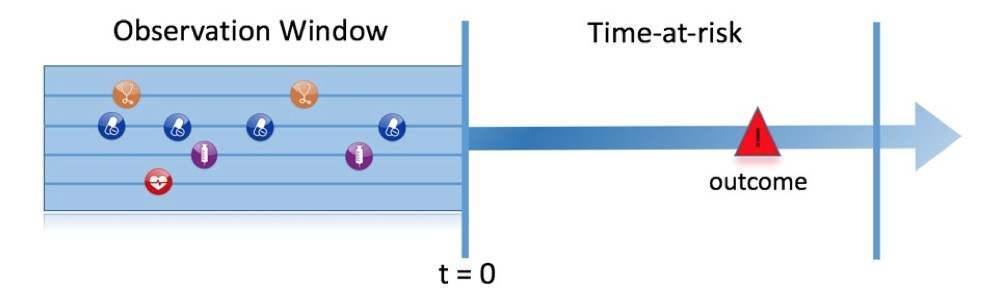
\includegraphics{Figure1.png}
\caption{The prediction problem}
\end{figure}

As shown in Figure 2, to define a prediction problem we have to define
t=0 by a Target Cohort (T), the outcome we like to predict by an outcome
cohort (O), and the time-at-risk (TAR). Furthermore, we have to make
design choices for the model we like to develop, and determine the
observational datasets to perform internal and external validation. This
conceptual framework works for all type of prediction problems, for
example those presented in Figure 3.

\begin{figure}
\centering
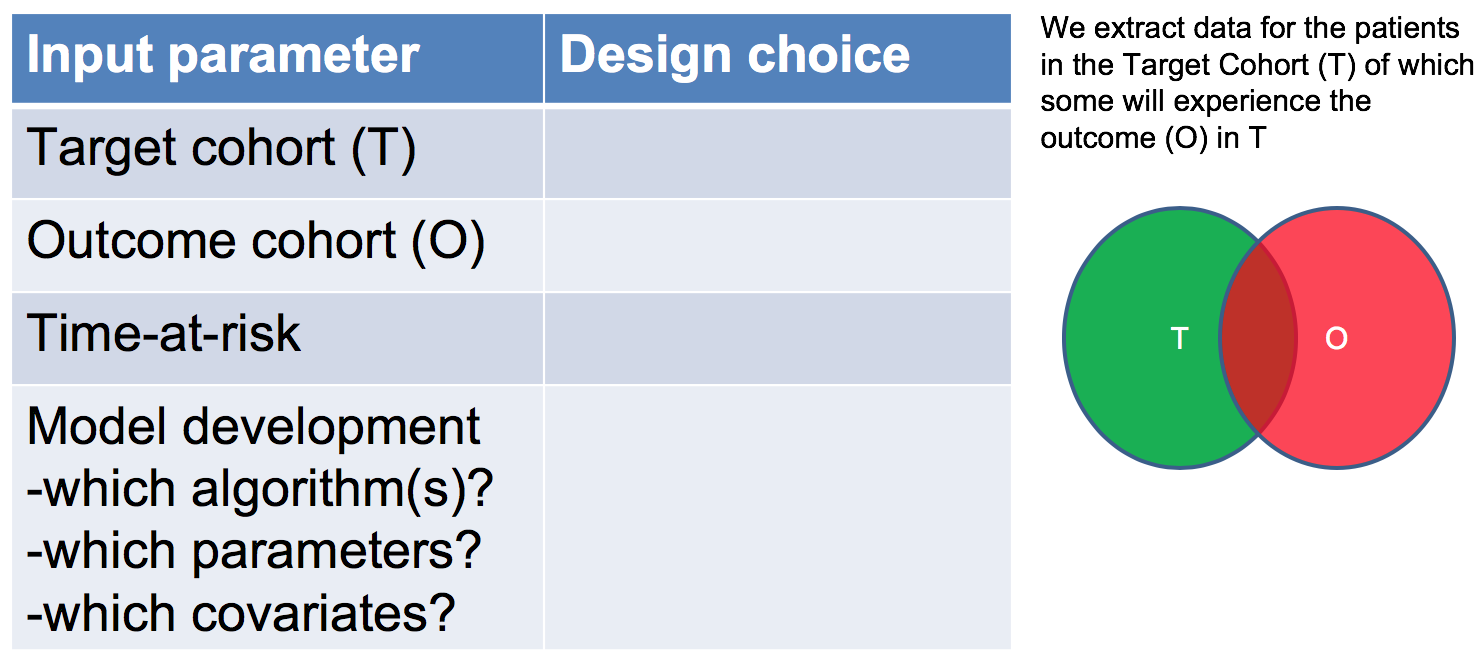
\includegraphics{studydesign.png}
\caption{Design choices}
\end{figure}

\begin{figure}
\centering
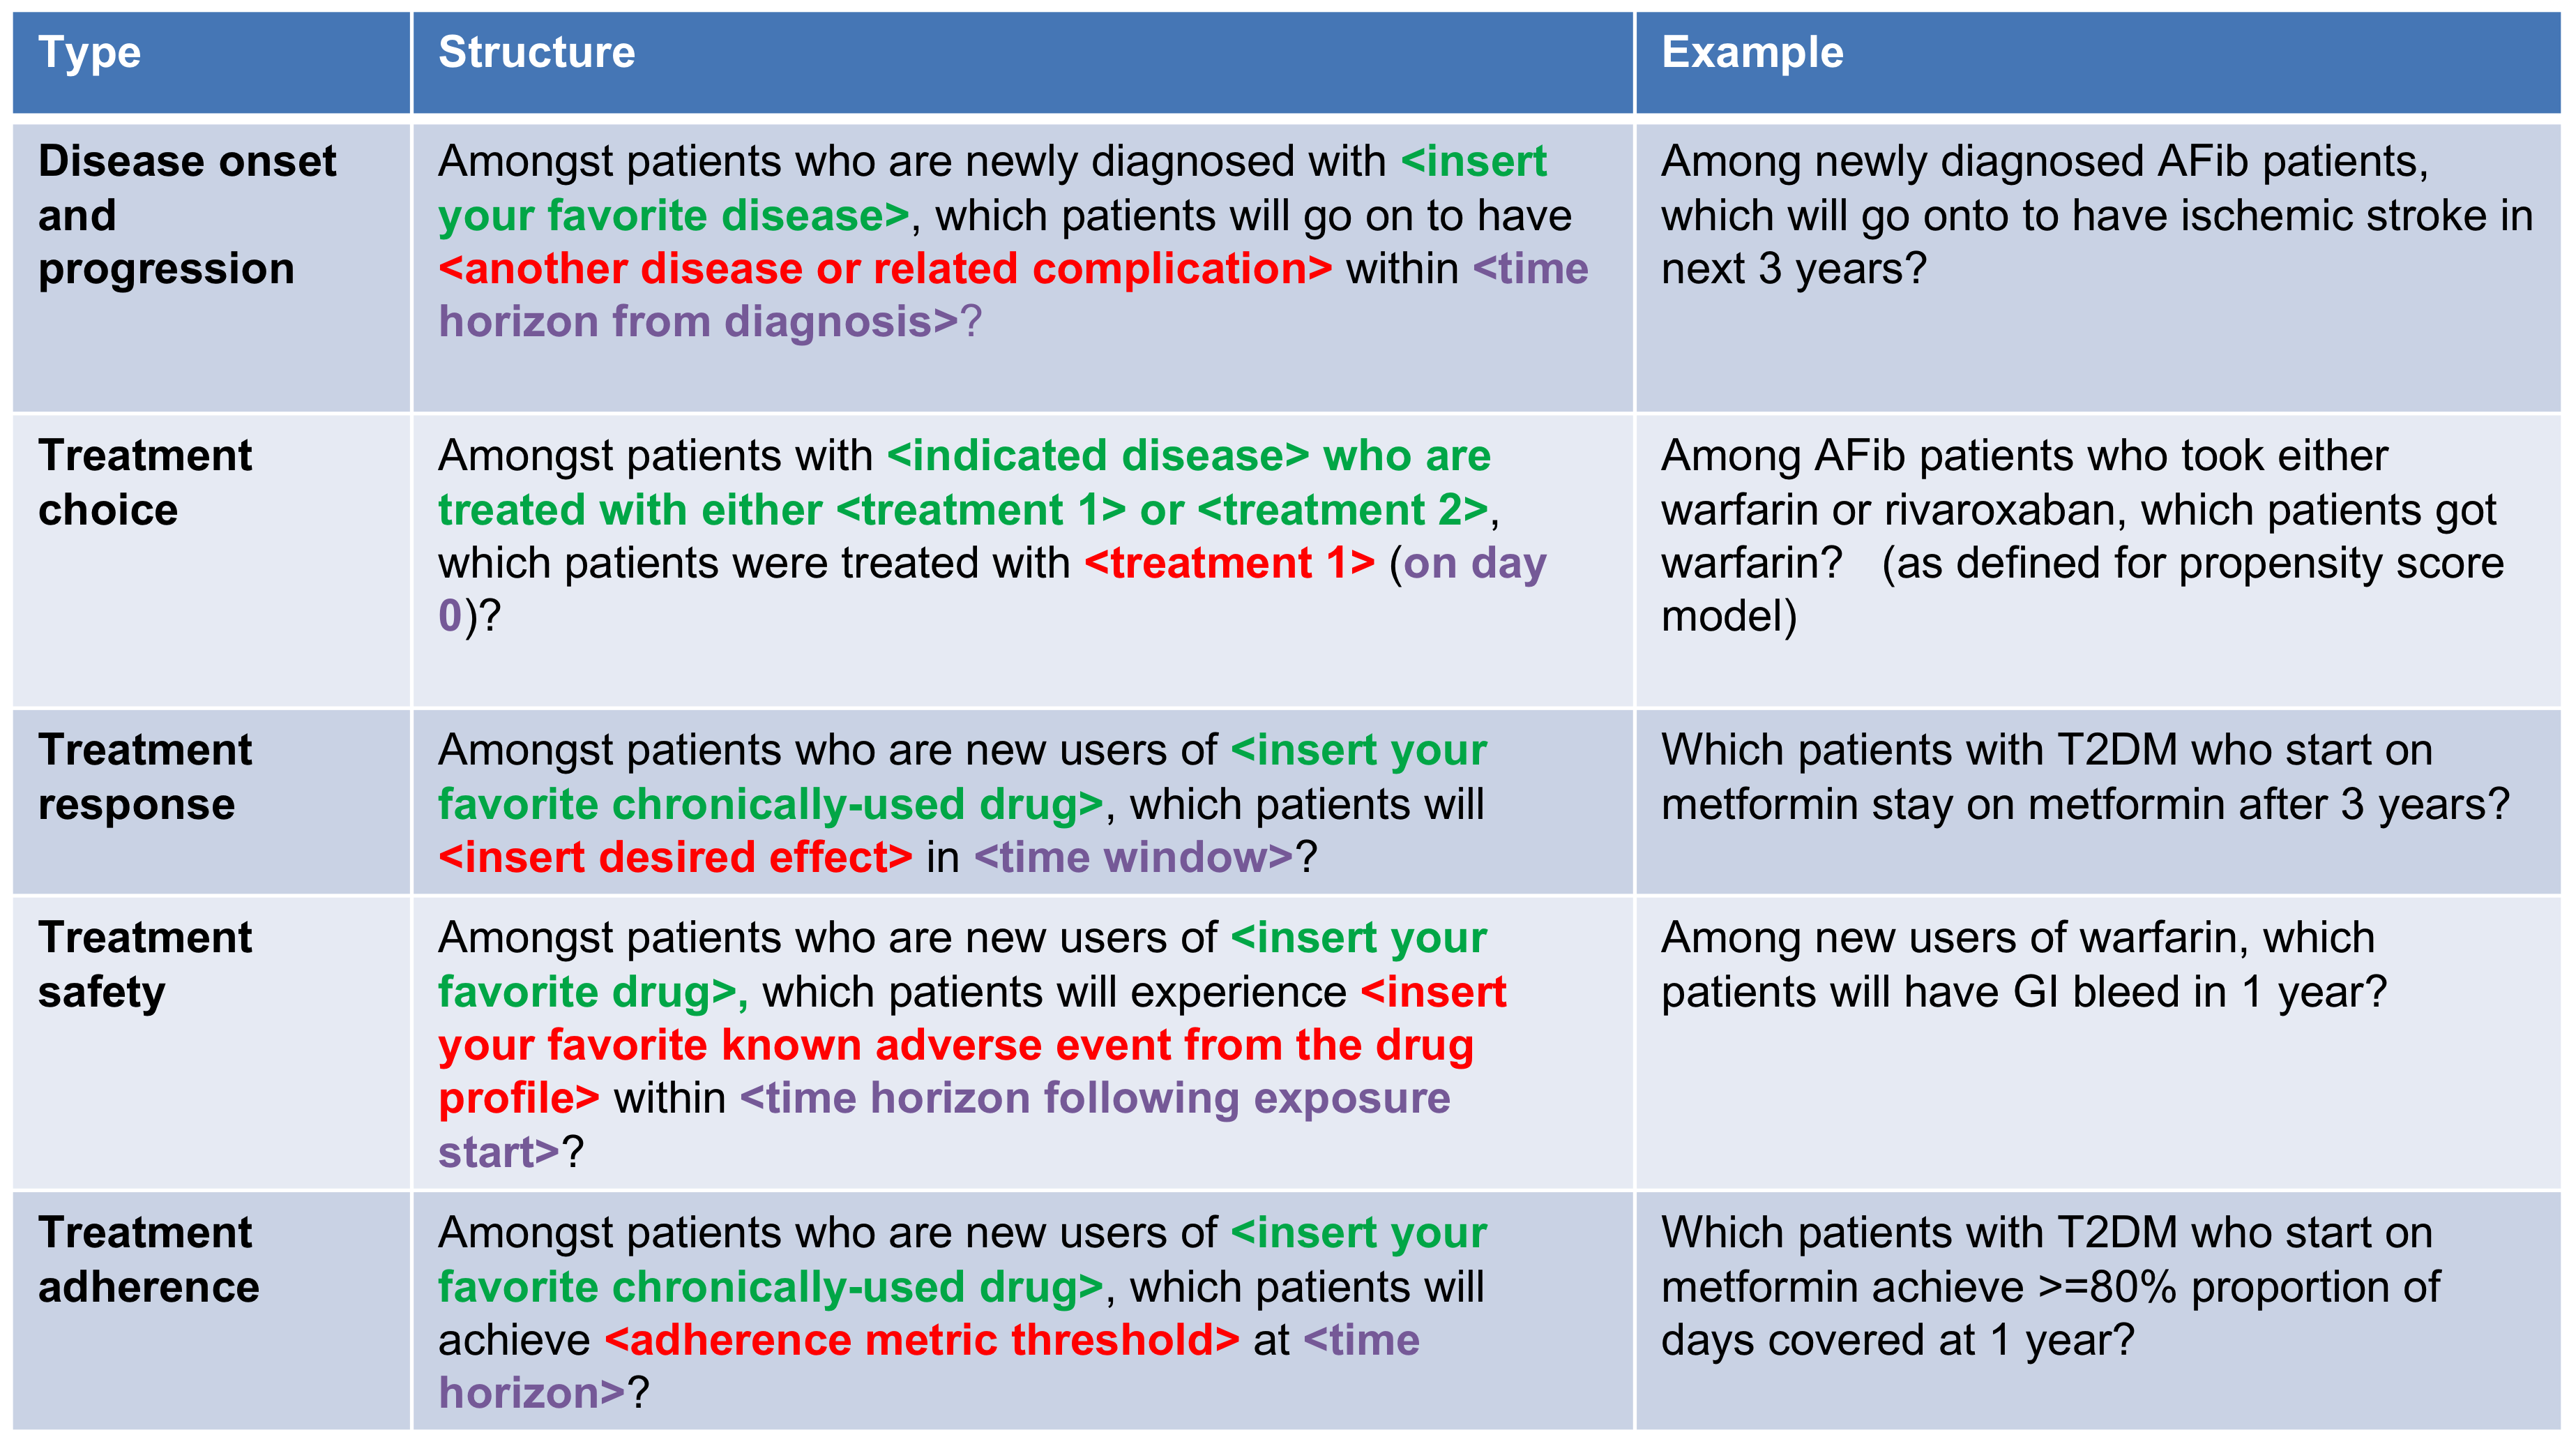
\includegraphics{problems.png}
\caption{Examples of prediction problems}
\end{figure}

This vignette describes how you can use the
\texttt{PatientLevelPrediction} package to build patient-level
predictive models. The package enables data extraction, model building,
and model evaluation using data from databases that are translated into
the OMOP CDM. In this vignette we assume you have installed the package
correctly using the
\href{https://github.com/OHDSI/PatientLevelPrediction/blob/master/inst/doc/InstallationGuide.pdf}{\texttt{InstallationGuide}}.

\hypertarget{study-specification}{%
\section{Study specification}\label{study-specification}}

We have to clearly specify our study upfront to be able to implement it.
This means we need to define the prediction problem we like to address,
in which population we will build the model, which model we will build
and how we will evaluate its performance. To guide you through this
process we will use a ``Disease onset and progression'' prediction type
as an example.

\hypertarget{problem-definition-1-stroke-in-afibrilation-patients}{%
\subsection{Problem definition 1: Stroke in afibrilation
patients}\label{problem-definition-1-stroke-in-afibrilation-patients}}

Atrial fibrillation is a disease characterized by an irregular heart
rate that can cause poor blood flow. Patients with atrial fibrillation
are at increased risk of ischemic stroke. Anticoagulation is a
recommended prophylaxis treatment strategy for patients at high risk of
stroke, though the underuse of anticoagulants and persistent severity of
ischemic stroke represents a substantial unmet medical need. Various
strategies have been developed to predict risk of ischemic stroke in
patients with atrial fibrillation. CHADS2 (Gage JAMA 2001) was developed
as a risk score based on history of congestive heart failure,
hypertension, age\textgreater=75, diabetes and stroke. CHADS2 was
initially derived using Medicare claims data, where it achieved good
discrimination (AUC=0.82). However, subsequent external validation
studies revealed the CHADS2 had substantially lower predictive accuracy
(Keogh Thromb Haemost 2011). Subsequent stroke risk calculators have
been developed and evaluated, including the extension of CHADS2Vasc. The
management of atrial fibrillation has evolved substantially over the
last decade, for various reasons that include the introduction of novel
oral anticoagulants. With these innovations has come a renewed interest
in greater precision medicine for stroke prevention.

We will apply the PatientLevelPrediction package to observational
healthcare data to address the following patient-level prediction
question:

Amongst patients who are newly diagnosed with Atrial Fibrillation, which
patients will go on to have Ischemic Stroke within 1 year?

We will define `patients who are newly diagnosed with Atrial
Fibrillation' as the first condition record of cardiac arrhythmia, which
is followed by another cardiac arrhythmia condition record, at least two
drug records for a drug used to treat arrhythmias, or a procedure to
treat arrhythmias. We will define `Ischemic stroke events' as ischemic
stroke condition records during an inpatient or ER visit; successive
records with \textgreater{} 180 day gap are considered independent
episodes.

\hypertarget{problem-definition-2-angioedema-in-ace-inhibitor-users}{%
\subsection{Problem definition 2: Angioedema in ACE inhibitor
users}\label{problem-definition-2-angioedema-in-ace-inhibitor-users}}

Angiotensin converting enzyme inhibitors (ACE inhibitors) are
medications used by patients with hypertension that widen the blood
vessles and therefore increse the amount of blood pumped by the heart
and decreases blood pressure. Ace inhibitors reduce a patients risk of
cardiovasular disease but can lead to drug-induced angioedema.

We will apply the PatientLevelPrediction package to observational
healthcare data to address the following patient-level prediction
question:

Amongst patients who are newly dispensed an ACE inhibitor, which
patients will go on to have angioedema within 1 year?

We will define `patients who are newly dispensed an ACE inhibitor' as
the first drug record of sny ACE inhibitor, {[}\ldots{]}which is
followed by another cardiac arrhythmia condition record, at least two
drug records for a drug used to treat arrhythmias, or a procedure to
treat arrhythmias. We will define `angioedema' as an angioedema
condition record.

\hypertarget{study-population-definition}{%
\subsection{Study population
definition}\label{study-population-definition}}

The final study population in which we will develop our model is often a
subset of the Target population, because we will e.g.~apply criteria
that are dependent on T and O or we want to do sensitivity analyses with
subpopulations of T. For this we have to answer the following questions:

\begin{itemize}
\item
  \emph{What is the minimum amount of observation time we require before
  the start of the target cohort?} This choice could depend on the
  available patient time in your training data, but also on the time you
  expect to be available in the data sources you want to apply the model
  on in the future. The longer the minimum observation time, the more
  baseline history time is available for each person to use for feature
  extraction, but the fewer patients will qualify for analysis.
  Moreover, there could be clinical reasons to choose a short or longer
  lookback period. For our example, we will use a prior history as
  lookback period (washout period).
\item
  \emph{Can patients enter the target cohort multiple times?} In the
  target cohort definition, a person may qualify for the cohort multiple
  times during different spans of time, for example if they had
  different episodes of a disease or separate periods of exposure to a
  medical product. The cohort definition does not necessarily apply a
  restriction to only let the patients enter once, but in the context of
  a particular patient-level prediction problem, a user may want to
  restrict the cohort to the first qualifying episode. In our example, a
  person could only enter the target cohort once since our criteria was
  based on first occurrence of atrial fibrillation.
\item
  \emph{Do we allow persons to enter the cohort if they experienced the
  outcome before?} Do we allow persons to enter the target cohort if
  they experienced the outcome before qualifying for the target cohort?
  Depending on the particular patient-level prediction problem, there
  may be a desire to predict `incident' first occurrence of an outcome,
  in which case patients who have previously experienced the outcome are
  not `at-risk' for having a first occurrence and therefore should be
  excluded from the target cohort. In other circumstances, there may be
  a desire to predict `prevalent' episodes, whereby patients with prior
  outcomes can be included in the analysis and the prior outcome itself
  can be a predictor of future outcomes. For our prediction example, the
  answer to this question is `Yes, allow persons with prior outcomes'
  because we know from the CHADS2 score that prior strokes are very
  predictive of future strokes. If this answer would have been `No' we
  also have to decide how long we would look back for previous
  occurrences of the outcome.
\item
  \emph{How do we define the period in which we will predict our outcome
  relative to the target cohort start?} We actually have to make two
  decisions to answer that question. First, does the time-at-risk window
  start at the date of the start of the target cohort or later?
  Arguments to make it start later could be that you want to avoid
  outcomes that were entered late in the record that actually occurred
  before the start of the target cohort or you want to leave a gap where
  interventions to prevent the outcome could theoretically be
  implemented. Second, you need to define the time-at-risk by setting
  the risk window end, as some specification of days offset relative to
  the target cohort start or end dates. For our problem we will predict
  in a `time-at-risk' window starting 1 day after the start of the
  target cohort up to 365 days later (to look for 1-year risk following
  atrial fibrillation diagnosis).
\item
  \emph{Do we require a minimum amount of time-at-risk?} We have to
  decide if we want to include patients that did not experience the
  outcome but did leave the database earlier than the end of our
  time-at-risk period. These patients may experience the outcome when we
  do not observe them. For our prediction problem we decide to answer
  this question with `Yes, require a mimimum time-at-risk' for that
  reason. Furthermore, we have to decide if this constraint also applies
  to persons who experienced the outcome or we will include all persons
  with the outcome irrespective of their total time at risk. For
  example, if the outcome is death, then persons with the outcome are
  likely censored before the full time-at-risk period is complete.
\end{itemize}

\hypertarget{model-development-settings}{%
\subsection{Model development
settings}\label{model-development-settings}}

To develop the model we have to decide which algorithm(s) we like to
train. We see the selection of the best algorithm for a certain
prediction problem as an empirical question, i.e.~you need to let the
data speak for itself and try different approaches to find the best one.
There is no algorithm that will work best for all problems (no free
lunch). In our package we therefore aim to implement many algorithms.
Furthermore, we made the system modular so you can add your own custom
algorithms as described in more detail in the
\href{Link\%20to\%20be\%20added}{\texttt{AddingCustomAlgorithms}}
vignette.

Our package currently contains the following algorithms to choose from:

\begin{longtable}[]{@{}lll@{}}
\toprule
\begin{minipage}[b]{0.11\columnwidth}\raggedright
Algorihm\strut
\end{minipage} & \begin{minipage}[b]{0.55\columnwidth}\raggedright
Description\strut
\end{minipage} & \begin{minipage}[b]{0.25\columnwidth}\raggedright
Hyper-parameters\strut
\end{minipage}\tabularnewline
\midrule
\endhead
\begin{minipage}[t]{0.11\columnwidth}\raggedright
Regularized Logistic Regression\strut
\end{minipage} & \begin{minipage}[t]{0.55\columnwidth}\raggedright
Lasso logistic regression belongs to the family of generalized linear
models, where a linear combination of the variables is learned and
finally a logistic function maps the linear combination to a value
between 0 and 1. The lasso regularization adds a cost based on model
complexity to the objective function when training the model. This cost
is the sum of the absolute values of the linear combination of the
coefficients. The model automatically performs feature selection by
minimizing this cost. We use the Cyclic coordinate descent for logistic,
Poisson and survival analysis (Cyclops) package to perform large-scale
regularized logistic regression:
\url{https://github.com/OHDSI/Cyclops}\strut
\end{minipage} & \begin{minipage}[t]{0.25\columnwidth}\raggedright
var (starting variance), seed\strut
\end{minipage}\tabularnewline
\begin{minipage}[t]{0.11\columnwidth}\raggedright
Gradient boosting machines\strut
\end{minipage} & \begin{minipage}[t]{0.55\columnwidth}\raggedright
Gradient boosting machines is a boosting ensemble technique and in our
framework it combines multiple decision trees. Boosting works by
iteratively adding decision trees but adds more weight to the
data-points that are misclassified by prior decision trees in the cost
function when training the next tree. We use Extreme Gradient Boosting,
which is an efficient implementation of the gradient boosting framework
implemented in the xgboost R package available from CRAN.\strut
\end{minipage} & \begin{minipage}[t]{0.25\columnwidth}\raggedright
ntree (number of trees), max depth (max levels in tree), min rows
(minimum data points in in node), learning rate, balance (balance class
labels), seed\strut
\end{minipage}\tabularnewline
\begin{minipage}[t]{0.11\columnwidth}\raggedright
Random forest\strut
\end{minipage} & \begin{minipage}[t]{0.55\columnwidth}\raggedright
Random forest is a bagging ensemble technique that combines multiple
decision trees. The idea behind bagging is to reduce the likelihood of
overfitting, by using weak classifiers, but combining multiple diverse
weak classifiers into a strong classifier. Random forest accomplishes
this by training multiple decision trees but only using a subset of the
variables in each tree and the subset of variables differ between trees.
Our packages uses the sklearn learn implementation of Random Forest in
python.\strut
\end{minipage} & \begin{minipage}[t]{0.25\columnwidth}\raggedright
mtry (number of features in each tree),ntree (number of trees), maxDepth
(max levels in tree), minRows (minimum data points in in node),balance
(balance class labels), seed\strut
\end{minipage}\tabularnewline
\begin{minipage}[t]{0.11\columnwidth}\raggedright
K-nearest neighbors\strut
\end{minipage} & \begin{minipage}[t]{0.55\columnwidth}\raggedright
K-nearest neighbors (KNN) is an algorithm that uses some metric to find
the K closest labelled data-points, given the specified metric, to a new
unlabelled data-point. The prediction of the new data-points is then the
most prevalent class of the K-nearest labelled data-points. There is a
sharing limitation of KNN, as the model requires labelled data to
perform the prediction on new data, and it is often not possible to
share this data across data sites.We included the BigKnn classifier
developed in OHDSI which is a large scale k-nearest neighbor classifier
using the Lucene search engine:
\url{https://github.com/OHDSI/BigKnn}\strut
\end{minipage} & \begin{minipage}[t]{0.25\columnwidth}\raggedright
k (number of neighbours),weighted (weight by inverse frequency)\strut
\end{minipage}\tabularnewline
\begin{minipage}[t]{0.11\columnwidth}\raggedright
Naive Bayes\strut
\end{minipage} & \begin{minipage}[t]{0.55\columnwidth}\raggedright
The Naive Bayes algorithm applies the Bayes theorem with the `naive'
assumption of conditional independence between every pair of features
given the value of the class variable. Based on the likelihood the data
belongs to a class and the prior distribution of the class, a posterior
distribution is obtained.\strut
\end{minipage} & \begin{minipage}[t]{0.25\columnwidth}\raggedright
none\strut
\end{minipage}\tabularnewline
\begin{minipage}[t]{0.11\columnwidth}\raggedright
AdaBoost\strut
\end{minipage} & \begin{minipage}[t]{0.55\columnwidth}\raggedright
AdaBoost is a boosting ensemble technique. Boosting works by iteratively
adding classifiers but adds more weight to the data-points that are
misclassified by prior classifiers in the cost function when training
the next classifier. We use the sklearn `AdaboostClassifier'
implementation in Python.\strut
\end{minipage} & \begin{minipage}[t]{0.25\columnwidth}\raggedright
nEstimators (the maximum number of estimators at which boosting is
terminated), learningRate (learning rate shrinks the contribution of
each classifier by learning\_rate. There is a trade-off between
learningRate and nEstimators)\strut
\end{minipage}\tabularnewline
\begin{minipage}[t]{0.11\columnwidth}\raggedright
Decision Tree\strut
\end{minipage} & \begin{minipage}[t]{0.55\columnwidth}\raggedright
A decision tree is a classifier that partitions the variable space using
individual tests selected using a greedy approach. It aims to find
partitions that have the highest information gain to separate the
classes. The decision tree can easily overfit by enabling a large number
of partitions (tree depth) and often needs some regularization (e.g.,
pruning or specifying hyper-parameters that limit the complexity of the
model). We use the sklearn `DecisionTreeClassifier' implementation in
Python.\strut
\end{minipage} & \begin{minipage}[t]{0.25\columnwidth}\raggedright
maxDepth (the maximum depth of the tree),
minSamplesSplit,minSamplesLeaf, minImpuritySplit (threshold for early
stopping in tree growth. A node will split if its impurity is above the
threshold, otherwise it is a leaf.), seed,classWeight (`Balance' or
`None')\strut
\end{minipage}\tabularnewline
\begin{minipage}[t]{0.11\columnwidth}\raggedright
Multilayer Perception\strut
\end{minipage} & \begin{minipage}[t]{0.55\columnwidth}\raggedright
Neural networks contain multiple layers that weight their inputs using a
non-linear function. The first layer is the input layer, the last layer
is the output layer the between are the hidden layers. Neural networks
are generally trained using feed forward back-propagation. This is when
you go through the network with a data-point and calculate the error
between the true label and predicted label, then go backwards through
the network and update the linear function weights based on the error.
This can also be performed as a batch, where multiple data-points are
fee\strut
\end{minipage} & \begin{minipage}[t]{0.25\columnwidth}\raggedright
size (the number of hidden nodes), alpha (the l2 regularisation),
seed\strut
\end{minipage}\tabularnewline
\begin{minipage}[t]{0.11\columnwidth}\raggedright
Deep Learning\strut
\end{minipage} & \begin{minipage}[t]{0.55\columnwidth}\raggedright
Deep learning such as deep nets, convolutional neural networks or
recurrent neural networks are similar to a neural network but have
multiple hidden layers that aim to learn latent representations useful
for prediction. In the seperate BuildingDeepLearningModels vignette we
describe these models and hyper-parameters in more detail\strut
\end{minipage} & \begin{minipage}[t]{0.25\columnwidth}\raggedright
see BuildingDeepLearningModels vignette\strut
\end{minipage}\tabularnewline
\bottomrule
\end{longtable}

Furthermore, we have to decide on the \textbf{covariates} that we will
use to train our model. This choice can be driven by domain knowledge of
available computational resources. In our example, we like to add the
Gender, Age, Conditions, Drugs Groups, and Visit Count. We also have to
specify in which time windows we will look and we decide to look in year
before and any time prior.

Finally, we have to define how we will train and test our model on our
data, i.e.~how we perform \textbf{internal validation}. For this we have
to decide how we divide our dataset in a training and testing dataset
and how we randomly assign patients to these two sets. Dependent on the
size of the training set we can decide how much data we like to use for
training, typically this is a 75\%, 25\% split. If you have very large
datasets you can use more data for training. To randomly assign patients
to the training and testing set, there are two commonly used approaches:

\begin{enumerate}
\def\labelenumi{\arabic{enumi}.}
\tightlist
\item
  split by person. In this case a random seed is used to assign the
  patient to either sets.
\item
  split by time. In this case a time point is used to split the persons,
  e.g.~75\% of the data is before and 25\% is after this date. The
  advantage of this is that you take into consideration that the health
  care system has changed over time.
\end{enumerate}

We now completely defined our studies and implement them:

\begin{itemize}
\tightlist
\item
  \protect\hyperlink{example1}{See example 1: Stroke in afibrilation
  patients}
\item
  \protect\hyperlink{example2}{See example 2: Agioedema in ACE inhibitor
  new users}
\end{itemize}

\hypertarget{example1}{%
\section{Example 1: Stroke in afibrilation patients}\label{example1}}

\hypertarget{study-specification-1}{%
\subsection{Study Specification}\label{study-specification-1}}

For our first prediction model we decide to start with a Regularized
Logistic Regression and will use the default parameters. We will do a
75\%-25\% split by person.

\begin{longtable}[]{@{}ll@{}}
\toprule
\begin{minipage}[b]{0.42\columnwidth}\raggedright
Definition\strut
\end{minipage} & \begin{minipage}[b]{0.52\columnwidth}\raggedright
Value\strut
\end{minipage}\tabularnewline
\midrule
\endhead
\begin{minipage}[t]{0.42\columnwidth}\raggedright
\textbf{Problem Definition}\strut
\end{minipage} & \begin{minipage}[t]{0.52\columnwidth}\raggedright
\strut
\end{minipage}\tabularnewline
\begin{minipage}[t]{0.42\columnwidth}\raggedright
Target Cohort (T)\strut
\end{minipage} & \begin{minipage}[t]{0.52\columnwidth}\raggedright
`Patients who are newly diagnosed with Atrial Fibrillation' defined as
the first condition record of cardiac arrhythmia, which is followed by
another cardiac arrhythmia condition record, at least two drug records
for a drug used to treat arrhythmias, or a procedure to treat
arrhythmias.\strut
\end{minipage}\tabularnewline
\begin{minipage}[t]{0.42\columnwidth}\raggedright
Outcome Cohort (O)\strut
\end{minipage} & \begin{minipage}[t]{0.52\columnwidth}\raggedright
`Ischemic stroke events' defined as ischemic stroke condition records
during an inpatient or ER visit; successive records with \textgreater{}
180 day gap are considered independent episodes.\strut
\end{minipage}\tabularnewline
\begin{minipage}[t]{0.42\columnwidth}\raggedright
Time-at-risk (TAR)\strut
\end{minipage} & \begin{minipage}[t]{0.52\columnwidth}\raggedright
1 day till 365 days from cohort start\strut
\end{minipage}\tabularnewline
\begin{minipage}[t]{0.42\columnwidth}\raggedright
\strut
\end{minipage} & \begin{minipage}[t]{0.52\columnwidth}\raggedright
\strut
\end{minipage}\tabularnewline
\begin{minipage}[t]{0.42\columnwidth}\raggedright
\textbf{Population Definition}\strut
\end{minipage} & \begin{minipage}[t]{0.52\columnwidth}\raggedright
\strut
\end{minipage}\tabularnewline
\begin{minipage}[t]{0.42\columnwidth}\raggedright
Washout Period\strut
\end{minipage} & \begin{minipage}[t]{0.52\columnwidth}\raggedright
1095\strut
\end{minipage}\tabularnewline
\begin{minipage}[t]{0.42\columnwidth}\raggedright
Enter the target cohort multiple times?\strut
\end{minipage} & \begin{minipage}[t]{0.52\columnwidth}\raggedright
No\strut
\end{minipage}\tabularnewline
\begin{minipage}[t]{0.42\columnwidth}\raggedright
Allow prior outcomes?\strut
\end{minipage} & \begin{minipage}[t]{0.52\columnwidth}\raggedright
Yes\strut
\end{minipage}\tabularnewline
\begin{minipage}[t]{0.42\columnwidth}\raggedright
Start of time-at-risk\strut
\end{minipage} & \begin{minipage}[t]{0.52\columnwidth}\raggedright
1 day\strut
\end{minipage}\tabularnewline
\begin{minipage}[t]{0.42\columnwidth}\raggedright
End of time-at-risk\strut
\end{minipage} & \begin{minipage}[t]{0.52\columnwidth}\raggedright
365 days\strut
\end{minipage}\tabularnewline
\begin{minipage}[t]{0.42\columnwidth}\raggedright
Require a minimum amount of time-at-risk?\strut
\end{minipage} & \begin{minipage}[t]{0.52\columnwidth}\raggedright
Yes (364 days)\strut
\end{minipage}\tabularnewline
\begin{minipage}[t]{0.42\columnwidth}\raggedright
\strut
\end{minipage} & \begin{minipage}[t]{0.52\columnwidth}\raggedright
\strut
\end{minipage}\tabularnewline
\begin{minipage}[t]{0.42\columnwidth}\raggedright
\textbf{Model Development}\strut
\end{minipage} & \begin{minipage}[t]{0.52\columnwidth}\raggedright
\strut
\end{minipage}\tabularnewline
\begin{minipage}[t]{0.42\columnwidth}\raggedright
Algorithm\strut
\end{minipage} & \begin{minipage}[t]{0.52\columnwidth}\raggedright
Regularized Logistic Regression\strut
\end{minipage}\tabularnewline
\begin{minipage}[t]{0.42\columnwidth}\raggedright
Hyper-parameters\strut
\end{minipage} & \begin{minipage}[t]{0.52\columnwidth}\raggedright
variance = 0.01 (Default)\strut
\end{minipage}\tabularnewline
\begin{minipage}[t]{0.42\columnwidth}\raggedright
Covariates\strut
\end{minipage} & \begin{minipage}[t]{0.52\columnwidth}\raggedright
Gender, Age, Conditions (ever before, \textless365), Drugs Groups (ever
before, \textless365), and Visit Count\strut
\end{minipage}\tabularnewline
\begin{minipage}[t]{0.42\columnwidth}\raggedright
Data split\strut
\end{minipage} & \begin{minipage}[t]{0.52\columnwidth}\raggedright
75\% train, 25\% test. Randomly assigned by person\strut
\end{minipage}\tabularnewline
\bottomrule
\end{longtable}

According to the best practices we need to make a protocol that
completely specifies how we plan to execute our study. This protocol
will be assessed by the governance boards of the participating data
sources in your network study. For this a template could be used but we
prefer to automate this process as much as possible by adding
functionality to automatically generate study protocol from a study
specification. We will discuss this in more detail later.

\hypertarget{study-implementation}{%
\subsection{Study implementation}\label{study-implementation}}

Now we have completely design our study we have to implement the study.
We have to generate the target and outcome cohorts and we need to
develop the R code to run against our CDM that will execute the full
study.

\hypertarget{cohort-instantiation}{%
\subsubsection{Cohort instantiation}\label{cohort-instantiation}}

For our study we need to know when a person enters the target and
outcome cohorts. This is stored in a table on the server that contains
the cohort start date and cohort end date for all subjects for a
specific cohort definition. This cohort table has a very simple
structure as shown below:

\begin{itemize}
\tightlist
\item
  \texttt{cohort\_definition\_id}, a unique identifier for
  distinguishing between different types of cohorts, e.g.~cohorts of
  interest and outcome cohorts.
\item
  \texttt{subject\_id}, a unique identifier corresponding to the
  \texttt{person\_id} in the CDM.
\item
  \texttt{cohort\_start\_date}, the date the subject enters the cohort.
\item
  \texttt{cohort\_end\_date}, the date the subject leaves the cohort.
\end{itemize}

How do we fill this table according to our cohort definitions? There are
two options for this:

\begin{enumerate}
\def\labelenumi{\arabic{enumi})}
\item
  use the interactive cohort builder tool in
  \href{www.github.com/OHDSI/ATLAS}{ATLAS} which can be used to create
  cohorts based on inclusion criteria and will automatically populate
  this cohort table.
\item
  write your own custom SQL statements to fill the cohort table.
\end{enumerate}

Both methods are described below for our example prediction problem.

\hypertarget{atlas-cohort-builder}{%
\subsubsection{ATLAS cohort builder}\label{atlas-cohort-builder}}

\begin{figure}
\centering
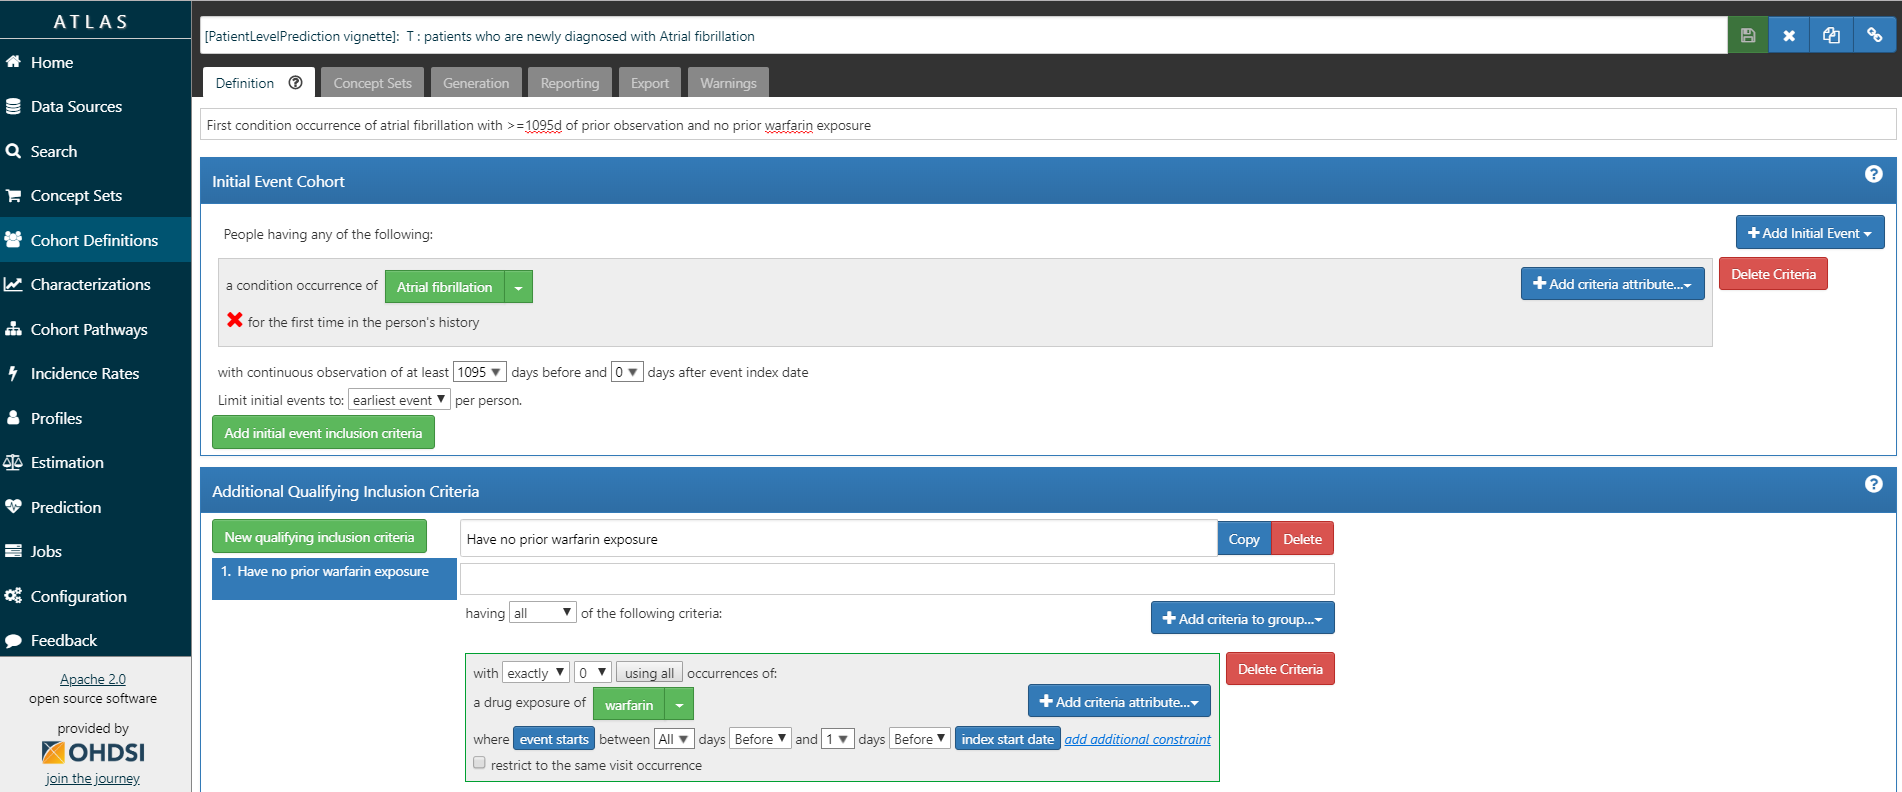
\includegraphics{example1/ATLAS_T.png}
\caption{Target Cohort Atrial Fibrillation}
\end{figure}

ATLAS allows you to define cohorts interactively by specifying cohort
entry and cohort exit criteria. Cohort entry criteria involve selecting
one or more initial events, which determine the start date for cohort
entry, and optionally specifying additional inclusion criteria which
filter to the qualifying events. Cohort exit criteria are applied to
each cohort entry record to determine the end date when the person's
episode no longer qualifies for the cohort. For the outcome cohort the
end date is less relevant. As an example, Figure 4 shows how we created
the Atrial Fibrillation cohort and Figure 5 shows how we created the
stroke cohort in ATLAS.

\begin{figure}
\centering
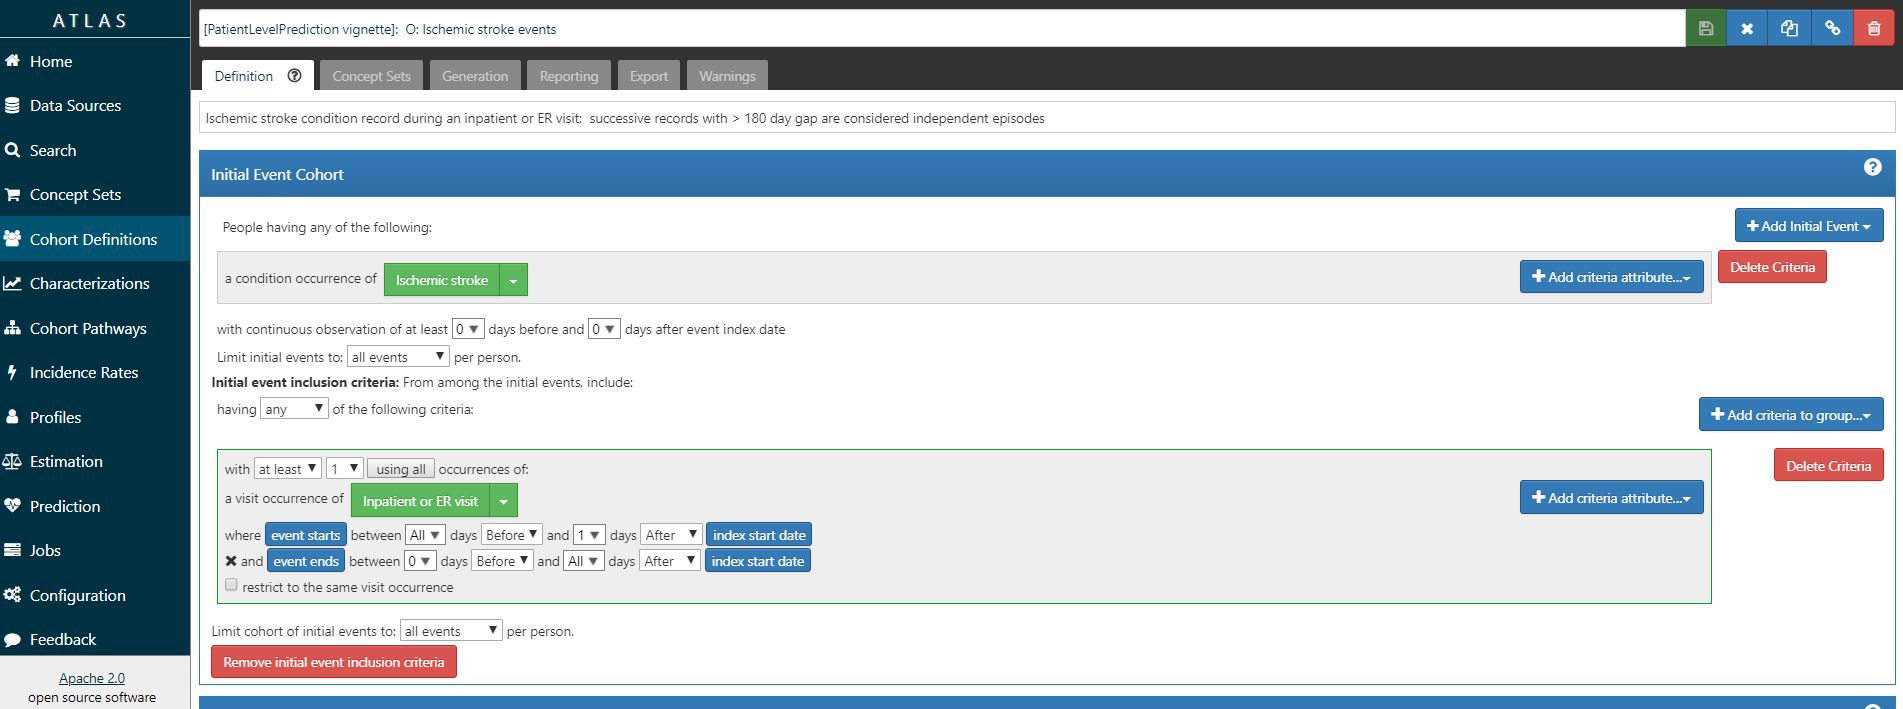
\includegraphics{example1/ATLAS_O.png}
\caption{Outcome Cohort Stroke}
\end{figure}

The T and O cohorts can be found here:

\begin{itemize}
\tightlist
\item
  Atrial Fibrillaton (T):
  \url{http://www.ohdsi.org/web/atlas/\#/cohortdefinition/1769447}
\item
  Stroke (O) :
  \url{http://www.ohdsi.org/web/atlas/\#/cohortdefinition/1769448}
\end{itemize}

In depth explanation of cohort creation in ATLAS is out of scope of this
vignette but can be found on the OHDSI wiki pages
\href{http://www.ohdsi.org/web/wiki/doku.php?id=documentation:software:atlas}{(link)}.

Note that when a cohort is created in ATLAS the cohortid is needed to
extract the data in R. The cohortid can be found at the top of the ATLAS
screen, e.g.~1769447 in Figure 4.

\hypertarget{custom-cohorts}{%
\subsubsection{Custom cohorts}\label{custom-cohorts}}

It is also possible to create cohorts without the use of ATLAS. Using
custom cohort code (SQL) you can make more advanced cohorts if needed.

For our example study, we need to create at table to hold the cohort
data and we need to create SQL code to instantiate this table for both
the AF and Stroke cohorts. Therefore, we create a file called
\emph{AfStrokeCohorts.sql} with the following contents:

\begin{Shaded}
\begin{Highlighting}[]
\CommentTok{/***********************************}
\CommentTok{File AfStrokeCohorts.sql }
\CommentTok{***********************************/}
\CommentTok{/*}
\CommentTok{Create a table to store the persons in the T and C cohort}
\CommentTok{*/}

\ControlFlowTok{IF}\NormalTok{ OBJECT_ID(}\StringTok{'@resultsDatabaseSchema.PLPAFibStrokeCohort'}\NormalTok{, }\StringTok{'U'}\NormalTok{) }\KeywordTok{IS} \KeywordTok{NOT} \KeywordTok{NULL} 
\KeywordTok{DROP} \KeywordTok{TABLE}\NormalTok{ @resultsDatabaseSchema.PLPAFibStrokeCohort;}

\KeywordTok{CREATE} \KeywordTok{TABLE}\NormalTok{ @resultsDatabaseSchema.PLPAFibStrokeCohort }
\NormalTok{( }
\NormalTok{cohort_definition_id }\DataTypeTok{INT}\NormalTok{, }
\NormalTok{subject_id BIGINT,}
\NormalTok{cohort_start_date }\DataTypeTok{DATE}\NormalTok{, }
\NormalTok{cohort_end_date }\DataTypeTok{DATE}
\NormalTok{);}


\CommentTok{/*}
\CommentTok{T cohort:  [PatientLevelPrediction vignette]:  T : patients who are newly }
\CommentTok{diagnosed with Atrial fibrillation}
\CommentTok{- persons with a condition occurrence record of 'Atrial fibrillation' or }
\CommentTok{any descendants, indexed at the first diagnosis}
\CommentTok{- who have >1095 days of prior observation before their first diagnosis}
\CommentTok{- and have no warfarin exposure any time prior to first AFib diagnosis}
\CommentTok{*/}
\KeywordTok{INSERT} \KeywordTok{INTO}\NormalTok{ @resultsDatabaseSchema.AFibStrokeCohort (cohort_definition_id, }
\NormalTok{subject_id, }
\NormalTok{cohort_start_date, }
\NormalTok{cohort_end_date)}
\KeywordTok{SELECT} \DecValTok{1} \KeywordTok{AS}\NormalTok{ cohort_definition_id,}
\NormalTok{AFib.person_id }\KeywordTok{AS}\NormalTok{ subject_id,}
\NormalTok{AFib.condition_start_date }\KeywordTok{AS}\NormalTok{ cohort_start_date,}
\NormalTok{observation_period.observation_period_end_date }\KeywordTok{AS}\NormalTok{ cohort_end_date}
\KeywordTok{FROM}
\NormalTok{(}
  \KeywordTok{SELECT}\NormalTok{ person_id, }\FunctionTok{min}\NormalTok{(condition_start_date) }\KeywordTok{as}\NormalTok{ condition_start_date}
  \KeywordTok{FROM}\NormalTok{ @cdmDatabaseSchema.condition_occurrence}
  \KeywordTok{WHERE}\NormalTok{ condition_concept_id }\KeywordTok{IN}\NormalTok{ (}\KeywordTok{SELECT}\NormalTok{ descendant_concept_id }\KeywordTok{FROM} 
\NormalTok{  @cdmDatabaseSchema.concept_ancestor }\KeywordTok{WHERE}\NormalTok{ ancestor_concept_id }\KeywordTok{IN} 
\NormalTok{  (}\DecValTok{313217} \CommentTok{/*atrial fibrillation*/}\NormalTok{))}
  \KeywordTok{GROUP} \KeywordTok{BY}\NormalTok{ person_id}
\NormalTok{) AFib}
  \KeywordTok{INNER} \KeywordTok{JOIN}\NormalTok{ @cdmDatabaseSchema.observation_period}
  \KeywordTok{ON}\NormalTok{ AFib.person_id }\OperatorTok{=}\NormalTok{ observation_period.person_id}
  \KeywordTok{AND}\NormalTok{ AFib.condition_start_date }\OperatorTok{>=}\NormalTok{ dateadd(dd,}\DecValTok{1095}\NormalTok{, }
\NormalTok{  observation_period.observation_period_start_date)}
  \KeywordTok{AND}\NormalTok{ AFib.condition_start_date }\OperatorTok{<=}\NormalTok{ observation_period.observation_period_end_date}
  \KeywordTok{LEFT} \KeywordTok{JOIN}
\NormalTok{  (}
  \KeywordTok{SELECT}\NormalTok{ person_id, }\FunctionTok{min}\NormalTok{(drug_exposure_start_date) }\KeywordTok{as}\NormalTok{ drug_exposure_start_date}
  \KeywordTok{FROM}\NormalTok{ @cdmDatabaseSchema.drug_exposure}
  \KeywordTok{WHERE}\NormalTok{ drug_concept_id }\KeywordTok{IN}\NormalTok{ (}\KeywordTok{SELECT}\NormalTok{ descendant_concept_id }\KeywordTok{FROM} 
\NormalTok{  @cdmDatabaseSchema.concept_ancestor }\KeywordTok{WHERE}\NormalTok{ ancestor_concept_id }\KeywordTok{IN} 
\NormalTok{  (}\DecValTok{1310149} \CommentTok{/*warfarin*/}\NormalTok{))}
  \KeywordTok{GROUP} \KeywordTok{BY}\NormalTok{ person_id}
\NormalTok{  ) warfarin}
  \KeywordTok{ON}\NormalTok{ Afib.person_id }\OperatorTok{=}\NormalTok{ warfarin.person_id}
  \KeywordTok{AND}\NormalTok{ Afib.condition_start_date }\OperatorTok{>}\NormalTok{ warfarin.drug_exposure_start_date}
  \KeywordTok{WHERE}\NormalTok{ warfarin.person_id }\KeywordTok{IS} \KeywordTok{NULL}
\NormalTok{  ;}
  
  \CommentTok{/*}
\CommentTok{  C cohort:  [PatientLevelPrediction vignette]:  O: Ischemic stroke events}
\CommentTok{  - inpatient visits that include a condition occurrence record for }
\CommentTok{  'cerebral infarction' and descendants, 'cerebral thrombosis', }
\CommentTok{  'cerebral embolism', 'cerebral artery occlusion' }
\CommentTok{  */}
  \KeywordTok{INSERT} \KeywordTok{INTO}\NormalTok{ @resultsDatabaseSchema.AFibStrokeCohort (cohort_definition_id, }
\NormalTok{  subject_id, }
\NormalTok{  cohort_start_date, }
\NormalTok{  cohort_end_date)}
  \KeywordTok{SELECT} \DecValTok{2} \KeywordTok{AS}\NormalTok{ cohort_definition_id,}
\NormalTok{  visit_occurrence.person_id }\KeywordTok{AS}\NormalTok{ subject_id,}
\NormalTok{  visit_occurrence.visit_start_date }\KeywordTok{AS}\NormalTok{ cohort_start_date,}
\NormalTok{  visit_occurrence.visit_end_date }\KeywordTok{AS}\NormalTok{ cohort_end_date}
  \KeywordTok{FROM}  
\NormalTok{  (}
  \KeywordTok{SELECT}\NormalTok{ person_id, condition_start_date}
  \KeywordTok{FROM}\NormalTok{ @cdmDatabaseSchema.condition_occurrence}
  \KeywordTok{WHERE}\NormalTok{ condition_concept_id }\KeywordTok{IN}\NormalTok{ (}\KeywordTok{SELECT} \KeywordTok{DISTINCT}\NormalTok{ descendant_concept_id }\KeywordTok{FROM} 
\NormalTok{  @cdmDatabaseSchema.concept_ancestor }\KeywordTok{WHERE}\NormalTok{ ancestor_concept_id }\KeywordTok{IN} 
\NormalTok{  (}\DecValTok{443454} \CommentTok{/*cerebral infarction*/}\NormalTok{) }\KeywordTok{OR}\NormalTok{ descendant_concept_id }\KeywordTok{IN} 
\NormalTok{  (}\DecValTok{441874} \CommentTok{/*cerebral thrombosis*/}\NormalTok{, }\DecValTok{375557} \CommentTok{/*cerebral embolism*/}\NormalTok{, }
  \DecValTok{372924} \CommentTok{/*cerebral artery occlusion*/}\NormalTok{))}
\NormalTok{  ) stroke}
  \KeywordTok{INNER} \KeywordTok{JOIN}\NormalTok{ @cdmDatabaseSchema.visit_occurrence}
  \KeywordTok{ON}\NormalTok{ stroke.person_id }\OperatorTok{=}\NormalTok{ visit_occurrence.person_id}
  \KeywordTok{AND}\NormalTok{ stroke.condition_start_date }\OperatorTok{>=}\NormalTok{ visit_occurrence.visit_start_date}
  \KeywordTok{AND}\NormalTok{ stroke.condition_start_date }\OperatorTok{<=}\NormalTok{ visit_occurrence.visit_end_date}
  \KeywordTok{AND}\NormalTok{ visit_occurrence.visit_concept_id }\KeywordTok{IN}\NormalTok{ (}\DecValTok{9201}\NormalTok{, }\DecValTok{262} \CommentTok{/*'Inpatient Visit'  or }
\CommentTok{  'Emergency Room and Inpatient Visit'*/}\NormalTok{)}
  \KeywordTok{GROUP} \KeywordTok{BY}\NormalTok{ visit_occurrence.person_id, visit_occurrence.visit_start_date, }
\NormalTok{  visit_occurrence.visit_end_date}
\NormalTok{  ;}
  
\end{Highlighting}
\end{Shaded}

This is parameterized SQL which can be used by the
\href{http://github.com/OHDSI/SqlRender}{\texttt{SqlRender}} package. We
use parameterized SQL so we do not have to pre-specify the names of the
CDM and result schemas. That way, if we want to run the SQL on a
different schema, we only need to change the parameter values; we do not
have to change the SQL code. By also making use of translation
functionality in \texttt{SqlRender}, we can make sure the SQL code can
be run in many different environments.

To execute this sql against our CDM we first need to tell R how to
connect to the server. \texttt{PatientLevelPrediction} uses the
\href{http://github.com/ohdsi/DatabaseConnector}{\texttt{DatabaseConnector}}
package, which provides a function called
\texttt{createConnectionDetails}. Type \texttt{?createConnectionDetails}
for the specific settings required for the various database management
systems (DBMS). For example, one might connect to a PostgreSQL database
using this code:

\begin{Shaded}
\begin{Highlighting}[]
\NormalTok{  connectionDetails <-}\StringTok{ }\KeywordTok{createConnectionDetails}\NormalTok{(}\DataTypeTok{dbms =} \StringTok{"postgresql"}\NormalTok{, }
  \DataTypeTok{server =} \StringTok{"localhost/ohdsi"}\NormalTok{, }
  \DataTypeTok{user =} \StringTok{"joe"}\NormalTok{, }
  \DataTypeTok{password =} \StringTok{"supersecret"}\NormalTok{)}
  
\NormalTok{  cdmDatabaseSchema <-}\StringTok{ "my_cdm_data"}
\NormalTok{  cohortsDatabaseSchema <-}\StringTok{ "my_results"}
\NormalTok{  cdmVersion <-}\StringTok{ "5"}
\end{Highlighting}
\end{Shaded}

The last three lines define the \texttt{cdmDatabaseSchema} and
\texttt{cohortsDatabaseSchema} variables, as well as the CDM version. We
will use these later to tell R where the data in CDM format live, where
we want to create the cohorts of interest, and what version CDM is used.
Note that for Microsoft SQL Server, databaseschemas need to specify both
the database and the schema, so for example
\texttt{cdmDatabaseSchema\ \textless{}-\ "my\_cdm\_data.dbo"}.

\begin{Shaded}
\begin{Highlighting}[]
  \KeywordTok{library}\NormalTok{(SqlRender)}
\NormalTok{  sql <-}\StringTok{ }\KeywordTok{readSql}\NormalTok{(}\StringTok{"AfStrokeCohorts.sql"}\NormalTok{)}
\NormalTok{  sql <-}\StringTok{ }\KeywordTok{renderSql}\NormalTok{(sql,}
  \DataTypeTok{cdmDatabaseSchema =}\NormalTok{ cdmDatabaseSchema,}
  \DataTypeTok{cohortsDatabaseSchema =}\NormalTok{ cohortsDatabaseSchema,}
  \DataTypeTok{post_time =} \DecValTok{30}\NormalTok{,}
  \DataTypeTok{pre_time =} \DecValTok{365}\NormalTok{)}\OperatorTok{$}\NormalTok{sql}
\NormalTok{  sql <-}\StringTok{ }\KeywordTok{translateSql}\NormalTok{(sql, }\DataTypeTok{targetDialect =}\NormalTok{ connectionDetails}\OperatorTok{$}\NormalTok{dbms)}\OperatorTok{$}\NormalTok{sql}
  
\NormalTok{  connection <-}\StringTok{ }\KeywordTok{connect}\NormalTok{(connectionDetails)}
  \KeywordTok{executeSql}\NormalTok{(connection, sql)}
\end{Highlighting}
\end{Shaded}

In this code, we first read the SQL from the file into memory. In the
next line, we replace four parameter names with the actual values. We
then translate the SQL into the dialect appropriate for the DBMS we
already specified in the \texttt{connectionDetails}. Next, we connect to
the server, and submit the rendered and translated SQL.

If all went well, we now have a table with the events of interest. We
can see how many events per type:

\begin{Shaded}
\begin{Highlighting}[]
\NormalTok{  sql <-}\StringTok{ }\KeywordTok{paste}\NormalTok{(}\StringTok{"SELECT cohort_definition_id, COUNT(*) AS count"}\NormalTok{,}
  \StringTok{"FROM @cohortsDatabaseSchema.AFibStrokeCohort"}\NormalTok{,}
  \StringTok{"GROUP BY cohort_definition_id"}\NormalTok{)}
\NormalTok{  sql <-}\StringTok{ }\KeywordTok{renderSql}\NormalTok{(sql, }\DataTypeTok{cohortsDatabaseSchema =}\NormalTok{ cohortsDatabaseSchema)}\OperatorTok{$}\NormalTok{sql}
\NormalTok{  sql <-}\StringTok{ }\KeywordTok{translateSql}\NormalTok{(sql, }\DataTypeTok{targetDialect =}\NormalTok{ connectionDetails}\OperatorTok{$}\NormalTok{dbms)}\OperatorTok{$}\NormalTok{sql}
  
  \KeywordTok{querySql}\NormalTok{(connection, sql)}
\end{Highlighting}
\end{Shaded}

\begin{verbatim}
##   cohort_definition_id  count
## 1                    1 527616
## 2                    2 221555
\end{verbatim}

\hypertarget{study-script-creation}{%
\subsubsection{Study script creation}\label{study-script-creation}}

In this section we assume that our cohorts have been created either by
using ATLAS or a custom SQL script. We will first explain how to create
an R script yourself that will execute our study as we have defined
earlier.

\hypertarget{data-extraction}{%
\subsubsection{Data extraction}\label{data-extraction}}

Now we can tell \texttt{PatientLevelPrediction} to extract all necessary
data for our analysis. This is done using the
\href{https://github.com/OHDSI/FeatureExtration}{\texttt{FeatureExtractionPackage}}.
In short the FeatureExtractionPackage allows you to specify which
features (covariates) need to be extracted, e.g.~all conditions and drug
exposures. It also supports the creation of custom covariates. For more
detailed information on the FeatureExtraction package see its
\href{https://github.com/OHDSI/FeatureExtration}{vignettes}. For our
example study we decided to use these settings:

\begin{Shaded}
\begin{Highlighting}[]
\NormalTok{  covariateSettings <-}\StringTok{ }\KeywordTok{createCovariateSettings}\NormalTok{(}\DataTypeTok{useDemographicsGender =} \OtherTok{TRUE}\NormalTok{,}
  \DataTypeTok{useDemographicsAge =} \OtherTok{TRUE}\NormalTok{,}
  \DataTypeTok{useConditionGroupEraLongTerm =} \OtherTok{TRUE}\NormalTok{,}
  \DataTypeTok{useConditionGroupEraAnyTimePrior =} \OtherTok{TRUE}\NormalTok{,}
  \DataTypeTok{useDrugGroupEraLongTerm =} \OtherTok{TRUE}\NormalTok{,}
  \DataTypeTok{useDrugGroupEraAnyTimePrior =} \OtherTok{TRUE}\NormalTok{,}
  \DataTypeTok{useVisitConceptCountLongTerm =} \OtherTok{TRUE}\NormalTok{,}
  \DataTypeTok{longTermStartDays =} \DecValTok{-365}\NormalTok{,}
  \DataTypeTok{endDays =} \DecValTok{-1}\NormalTok{)}
\end{Highlighting}
\end{Shaded}

The final step for extracting the data is to run the \texttt{getPlpData}
function and input the connection details, the database schema where the
cohorts are stored, the cohort definition ids for the cohort and
outcome, and the washoutPeriod which is the minimum number of days prior
to cohort index date that the person must have been observed to be
included into the data, and finally input the previously constructed
covariate settings.

\begin{Shaded}
\begin{Highlighting}[]
\NormalTok{  plpData <-}\StringTok{ }\KeywordTok{getPlpData}\NormalTok{(}\DataTypeTok{connectionDetails =}\NormalTok{ connectionDetails,}
  \DataTypeTok{cdmDatabaseSchema =}\NormalTok{ cdmDatabaseSchema,}
  \DataTypeTok{cohortDatabaseSchema =}\NormalTok{ resultsDatabaseSchema,}
  \DataTypeTok{cohortTable =} \StringTok{'AFibStrokeCohort'}\NormalTok{,}
  \DataTypeTok{cohortId =} \DecValTok{1}\NormalTok{,}
  \DataTypeTok{covariateSettings =}\NormalTok{ covariateSettings,}
  \DataTypeTok{outcomeDatabaseSchema =}\NormalTok{ resultsDatabaseSchema,}
  \DataTypeTok{outcomeTable =} \StringTok{'AFibStrokeCohort'}\NormalTok{,}
  \DataTypeTok{outcomeIds =} \DecValTok{2}\NormalTok{,}
  \DataTypeTok{sampleSize =} \DecValTok{10000}
\NormalTok{  )}
\end{Highlighting}
\end{Shaded}

Note that if the cohorts are created in ATLAS its corresponding cohort
database schema needs to be selected. There are many additional
parameters for the \texttt{getPlpData} function which are all documented
in the \texttt{PatientLevelPrediction} manual. The resulting
\texttt{plpData} object uses the package \texttt{ff} to store
information in a way that ensures R does not run out of memory, even
when the data are large.

Creating the \texttt{plpData} object can take considerable computing
time, and it is probably a good idea to save it for future sessions.
Because \texttt{plpData} uses \texttt{ff}, we cannot use R's regular
save function. Instead, we'll have to use the \texttt{savePlpData()}
function:

\begin{Shaded}
\begin{Highlighting}[]
\KeywordTok{savePlpData}\NormalTok{(plpData, }\StringTok{"stroke_in_af_data"}\NormalTok{)}
\end{Highlighting}
\end{Shaded}

We can use the \texttt{loadPlpData()} function to load the data in a
future session.

\hypertarget{additional-inclusion-criteria}{%
\subsubsection{Additional inclusion
criteria}\label{additional-inclusion-criteria}}

To completely define the prediction problem the final study population
is obtained by applying additional constraints on the two earlier
defined cohorts, e.g., a minumim time at risk can be enforced
(\texttt{requireTimeAtRisk,\ minTimeAtRisk}) and we can specify if this
also applies to patients with the outcome (\texttt{includeAllOutcomes}).
Here we also specify the start and end of the risk window relative to
target cohort start. For example, if we like the risk window to start 30
days after the at-risk cohort start and end a year later we can set
\texttt{riskWindowStart\ =\ 30} and \texttt{riskWindowEnd\ =\ 365}. In
some cases the risk window needs to start at the cohort end date. This
can be achieved by setting \texttt{addExposureToStart\ =\ TRUE} which
adds the cohort (exposure) time to the start date.

In Appendix 1, we demonstrate the effect of these settings on the subset
of the persons in the target cohort that end up in the final study
population.

In the example below all the settings we defined for our study are
imposed:

\begin{Shaded}
\begin{Highlighting}[]
\NormalTok{  population <-}\StringTok{ }\KeywordTok{createStudyPopulation}\NormalTok{(}\DataTypeTok{plpData =}\NormalTok{ plpData,}
  \DataTypeTok{outcomeId =} \DecValTok{2}\NormalTok{,}
  \DataTypeTok{washoutPeriod =} \DecValTok{1095}\NormalTok{,}
  \DataTypeTok{firstExposureOnly =} \OtherTok{FALSE}\NormalTok{,}
  \DataTypeTok{removeSubjectsWithPriorOutcome =} \OtherTok{FALSE}\NormalTok{,}
  \DataTypeTok{priorOutcomeLookback =} \DecValTok{1}\NormalTok{,}
  \DataTypeTok{riskWindowStart =} \DecValTok{1}\NormalTok{,}
  \DataTypeTok{riskWindowEnd =} \DecValTok{365}\NormalTok{,}
  \DataTypeTok{addExposureDaysToStart =} \OtherTok{FALSE}\NormalTok{,}
  \DataTypeTok{addExposureDaysToEnd =} \OtherTok{FALSE}\NormalTok{,}
  \DataTypeTok{minTimeAtRisk =} \DecValTok{364}\NormalTok{,}
  \DataTypeTok{requireTimeAtRisk =} \OtherTok{TRUE}\NormalTok{,}
  \DataTypeTok{includeAllOutcomes =} \OtherTok{TRUE}\NormalTok{,}
  \DataTypeTok{verbosity =} \StringTok{"DEBUG"}
\NormalTok{  )}
\end{Highlighting}
\end{Shaded}

\hypertarget{model-development}{%
\subsubsection{Model Development}\label{model-development}}

In the set function of an algorithm the user can specify a list of
eligible values for each hyper-parameter. All possible combinations of
the hyper-parameters are included in a so-called grid search using
cross-validation on the training set. If a user does not specify any
value then the default value is used instead.

For example, if we use the following settings for the
gradientBoostingMachine: ntrees=c(100,200), maxDepth=4 the grid search
will apply the gradient boosting machine algorithm with ntrees=100 and
maxDepth=4 plus the default settings for other hyper-parameters and
ntrees=200 and maxDepth=4 plus the default settings for other
hyper-parameters. The hyper-parameters that lead to the
bestcross-validation performance will then be chosen for the final
model. For our problem we choose to build a logistic regression model
with the default hyper-parameters

\begin{Shaded}
\begin{Highlighting}[]
\NormalTok{lrModel <-}\StringTok{ }\KeywordTok{setLassoLogisticRegression}\NormalTok{()}
\end{Highlighting}
\end{Shaded}

The \texttt{runPlP} function uses the population, \texttt{plpData}, and
model settings to train and evaluate the model. We can use the testSplit
(person/time) and testFraction parameters to split the data in a
75\%-25\% split and run the patient-level prediction pipeline:

\begin{Shaded}
\begin{Highlighting}[]
\NormalTok{  lrResults <-}\StringTok{ }\KeywordTok{runPlp}\NormalTok{(population, plpData, }\DataTypeTok{modelSettings =}\NormalTok{ lrModel, }\DataTypeTok{testSplit=}\StringTok{'stratified'}\NormalTok{, }
  \DataTypeTok{testFraction=}\FloatTok{0.25}\NormalTok{, }\DataTypeTok{nfold=}\DecValTok{2}\NormalTok{, }\DataTypeTok{splitSeed =} \DecValTok{1234}\NormalTok{)}
\end{Highlighting}
\end{Shaded}

Under the hood the package will now use the
\href{www.github.com/OHDSI/Cyclops}{\texttt{Cyclops}} package to fit a
large-scale regularized regression using 75\% of the data and will
evaluate the model on the remaining 25\%. A results data structure is
returned containing information about the model, its performance etc.

In the runPlp function there are several parameters to save the plpData,
plpResults, plpPlots, evaluation etc. which are all set to True by
default. However, there is also some functionality to this manually.

You can save the model using:

\begin{Shaded}
\begin{Highlighting}[]
\KeywordTok{savePlpModel}\NormalTok{(lrResults}\OperatorTok{$}\NormalTok{model, }\DataTypeTok{dirPath =} \KeywordTok{file.path}\NormalTok{(}\KeywordTok{getwd}\NormalTok{(), }\StringTok{"model"}\NormalTok{))}
\end{Highlighting}
\end{Shaded}

You can load the model using:

\begin{Shaded}
\begin{Highlighting}[]
\NormalTok{plpModel <-}\StringTok{ }\KeywordTok{loadPlpModel}\NormalTok{(}\KeywordTok{file.path}\NormalTok{(}\KeywordTok{getwd}\NormalTok{(), }\StringTok{"model"}\NormalTok{))}
\end{Highlighting}
\end{Shaded}

You can also save the full results structure using:

\begin{Shaded}
\begin{Highlighting}[]
\KeywordTok{savePlpResult}\NormalTok{(lrResults, }\DataTypeTok{location =} \KeywordTok{file.path}\NormalTok{(}\KeywordTok{getwd}\NormalTok{(), }\StringTok{"lr"}\NormalTok{))}
\end{Highlighting}
\end{Shaded}

To load the full results structure use:

\begin{Shaded}
\begin{Highlighting}[]
\NormalTok{lrResults <-}\StringTok{ }\KeywordTok{loadPlpResult}\NormalTok{(}\KeywordTok{file.path}\NormalTok{(}\KeywordTok{getwd}\NormalTok{(), }\StringTok{"lr"}\NormalTok{))}
\end{Highlighting}
\end{Shaded}

\newpage

\hypertarget{example2}{%
\section{Example 2: Angioedema in ACE inhibitor users}\label{example2}}

\hypertarget{study-specification-2}{%
\subsection{Study Specification}\label{study-specification-2}}

\begin{longtable}[]{@{}ll@{}}
\toprule
\begin{minipage}[b]{0.42\columnwidth}\raggedright
Definition\strut
\end{minipage} & \begin{minipage}[b]{0.52\columnwidth}\raggedright
Value\strut
\end{minipage}\tabularnewline
\midrule
\endhead
\begin{minipage}[t]{0.42\columnwidth}\raggedright
\textbf{Problem Definition}\strut
\end{minipage} & \begin{minipage}[t]{0.52\columnwidth}\raggedright
\strut
\end{minipage}\tabularnewline
\begin{minipage}[t]{0.42\columnwidth}\raggedright
Target Cohort (T)\strut
\end{minipage} & \begin{minipage}[t]{0.52\columnwidth}\raggedright
`Patients who are newly dispensed an ACE inhibitor' defined as the first
drug record of any ACE inhibitor\strut
\end{minipage}\tabularnewline
\begin{minipage}[t]{0.42\columnwidth}\raggedright
Outcome Cohort (O)\strut
\end{minipage} & \begin{minipage}[t]{0.52\columnwidth}\raggedright
`Angioedema' defined as an angioedema condition record during an
inpatient or ER visit\strut
\end{minipage}\tabularnewline
\begin{minipage}[t]{0.42\columnwidth}\raggedright
Time-at-risk (TAR)\strut
\end{minipage} & \begin{minipage}[t]{0.52\columnwidth}\raggedright
1 day till 365 days from cohort start\strut
\end{minipage}\tabularnewline
\begin{minipage}[t]{0.42\columnwidth}\raggedright
\strut
\end{minipage} & \begin{minipage}[t]{0.52\columnwidth}\raggedright
\strut
\end{minipage}\tabularnewline
\begin{minipage}[t]{0.42\columnwidth}\raggedright
\textbf{Population Definition}\strut
\end{minipage} & \begin{minipage}[t]{0.52\columnwidth}\raggedright
\strut
\end{minipage}\tabularnewline
\begin{minipage}[t]{0.42\columnwidth}\raggedright
Washout Period\strut
\end{minipage} & \begin{minipage}[t]{0.52\columnwidth}\raggedright
365\strut
\end{minipage}\tabularnewline
\begin{minipage}[t]{0.42\columnwidth}\raggedright
Enter the target cohort multiple times?\strut
\end{minipage} & \begin{minipage}[t]{0.52\columnwidth}\raggedright
No\strut
\end{minipage}\tabularnewline
\begin{minipage}[t]{0.42\columnwidth}\raggedright
Allow prior outcomes?\strut
\end{minipage} & \begin{minipage}[t]{0.52\columnwidth}\raggedright
No\strut
\end{minipage}\tabularnewline
\begin{minipage}[t]{0.42\columnwidth}\raggedright
Start of time-at-risk\strut
\end{minipage} & \begin{minipage}[t]{0.52\columnwidth}\raggedright
1 day\strut
\end{minipage}\tabularnewline
\begin{minipage}[t]{0.42\columnwidth}\raggedright
End of time-at-risk\strut
\end{minipage} & \begin{minipage}[t]{0.52\columnwidth}\raggedright
365 days\strut
\end{minipage}\tabularnewline
\begin{minipage}[t]{0.42\columnwidth}\raggedright
Require a minimum amount of time-at-risk?\strut
\end{minipage} & \begin{minipage}[t]{0.52\columnwidth}\raggedright
Yes (364 days)\strut
\end{minipage}\tabularnewline
\begin{minipage}[t]{0.42\columnwidth}\raggedright
\strut
\end{minipage} & \begin{minipage}[t]{0.52\columnwidth}\raggedright
\strut
\end{minipage}\tabularnewline
\begin{minipage}[t]{0.42\columnwidth}\raggedright
\textbf{Model Development}\strut
\end{minipage} & \begin{minipage}[t]{0.52\columnwidth}\raggedright
\strut
\end{minipage}\tabularnewline
\begin{minipage}[t]{0.42\columnwidth}\raggedright
Algorithm\strut
\end{minipage} & \begin{minipage}[t]{0.52\columnwidth}\raggedright
Gradient Boosting Machine\strut
\end{minipage}\tabularnewline
\begin{minipage}[t]{0.42\columnwidth}\raggedright
Hyper-parameters\strut
\end{minipage} & \begin{minipage}[t]{0.52\columnwidth}\raggedright
ntree:5000, max depth:4 or 7 or 10 and learning rate: 0.001 or 0.01 or
0.1 or 0.9\strut
\end{minipage}\tabularnewline
\begin{minipage}[t]{0.42\columnwidth}\raggedright
Covariates\strut
\end{minipage} & \begin{minipage}[t]{0.52\columnwidth}\raggedright
Gender, Age, Conditions (ever before, \textless365), Drugs Groups (ever
before, \textless365), and Visit Count\strut
\end{minipage}\tabularnewline
\begin{minipage}[t]{0.42\columnwidth}\raggedright
Data split\strut
\end{minipage} & \begin{minipage}[t]{0.52\columnwidth}\raggedright
75\% train, 25\% test. Randomly assigned by person\strut
\end{minipage}\tabularnewline
\bottomrule
\end{longtable}

According to the best practices we need to make a protocol that
completely specifies how we plan to execute our study. This protocol
will be assessed by the governance boards of the participating data
sources in your network study. For this a template could be used but we
prefer to automate this process as much as possible by adding
functionality to automatically generate study protocol from a study
specification. We will discuss this in more detail later.

\hypertarget{study-implementation-1}{%
\subsection{Study implementation}\label{study-implementation-1}}

Now we have completely design our study we have to implement the study.
We have to generate the target and outcome cohorts and we need to
develop the R code to run against our CDM that will execute the full
study.

\hypertarget{cohort-instantiation-1}{%
\subsubsection{Cohort instantiation}\label{cohort-instantiation-1}}

For our study we need to know when a person enters the target and
outcome cohorts. This is stored in a table on the server that contains
the cohort start date and cohort end date for all subjects for a
specific cohort definition. This cohort table has a very simple
structure as shown below:

\begin{itemize}
\tightlist
\item
  \texttt{cohort\_definition\_id}, a unique identifier for
  distinguishing between different types of cohorts, e.g.~cohorts of
  interest and outcome cohorts.
\item
  \texttt{subject\_id}, a unique identifier corresponding to the
  \texttt{person\_id} in the CDM.
\item
  \texttt{cohort\_start\_date}, the date the subject enters the cohort.
\item
  \texttt{cohort\_end\_date}, the date the subject leaves the cohort.
\end{itemize}

How do we fill this table according to our cohort definitions? There are
two options for this:

\begin{enumerate}
\def\labelenumi{\arabic{enumi})}
\item
  use the interactive cohort builder tool in
  \href{www.github.com/OHDSI/ATLAS}{ATLAS} which can be used to create
  cohorts based on inclusion criteria and will automatically populate
  this cohort table.
\item
  write your own custom SQL statements to fill the cohort table.
\end{enumerate}

Both methods are described below for our example prediction problem.

\hypertarget{atlas-cohort-builder-1}{%
\subsubsection{ATLAS cohort builder}\label{atlas-cohort-builder-1}}

\begin{figure}
\centering
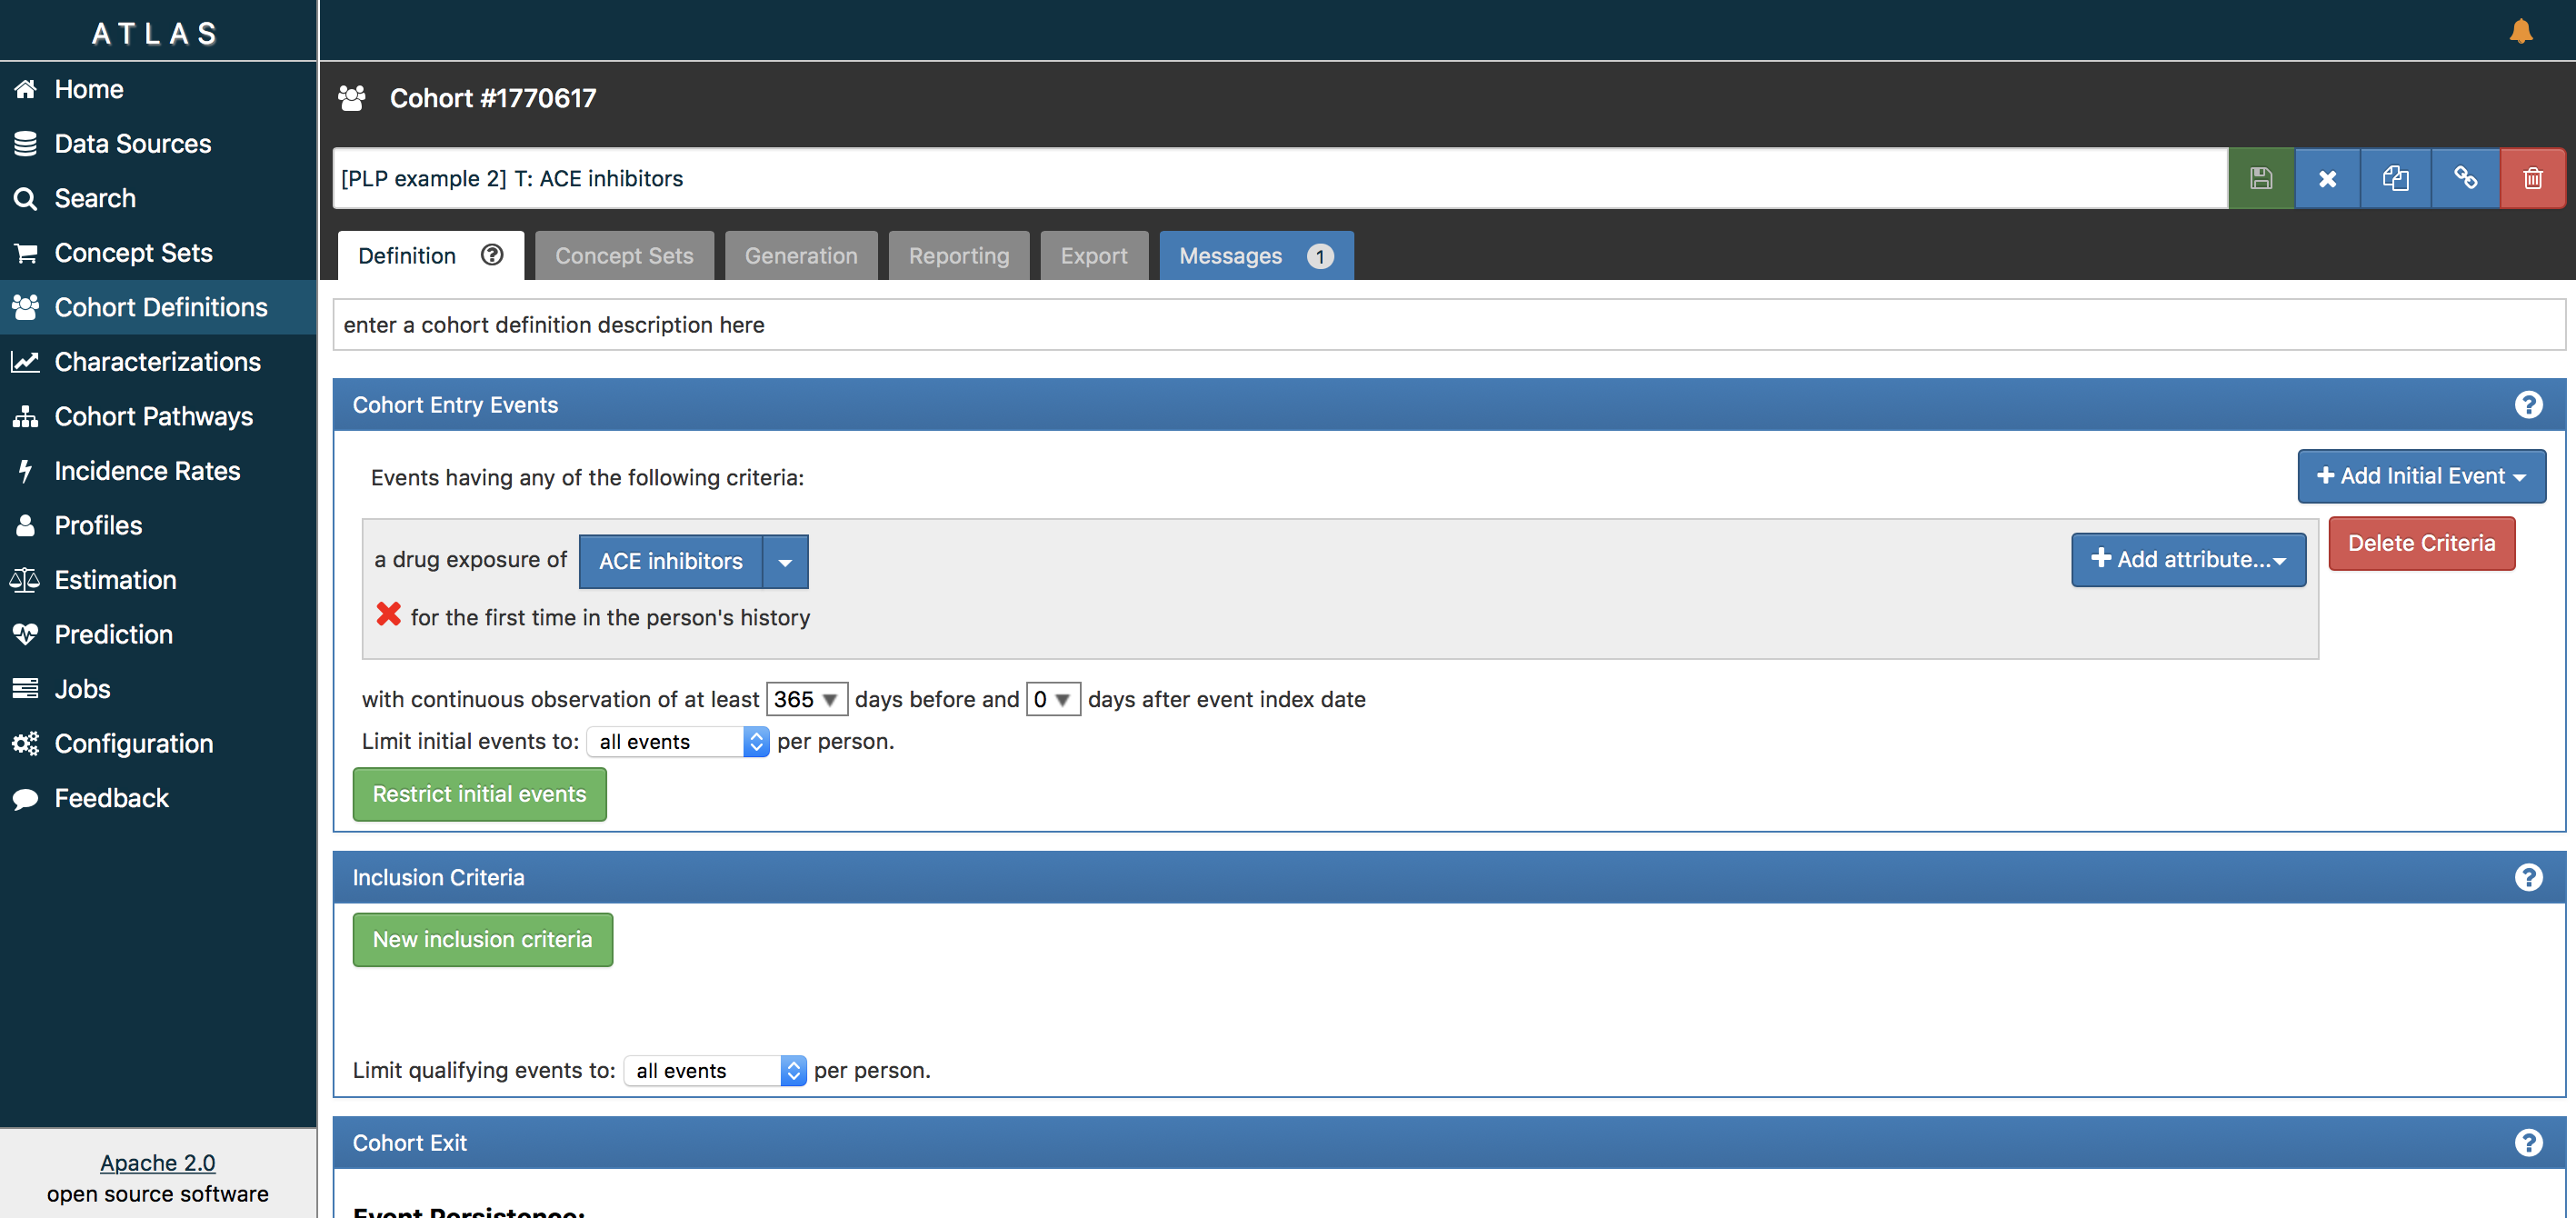
\includegraphics{example2/aceinhibitors.png}
\caption{Target Cohort ACE inhibitors}
\end{figure}

ATLAS allows you to define cohorts interactively by specifying cohort
entry and cohort exit criteria. Cohort entry criteria involve selecting
one or more initial events, which determine the start date for cohort
entry, and optionally specifying additional inclusion criteria which
filter to the qualifying events. Cohort exit criteria are applied to
each cohort entry record to determine the end date when the person's
episode no longer qualifies for the cohort. For the outcome cohort the
end date is less relevant. As an example, Figure 6 shows how we created
the ACE inhibitors cohort and Figure 7 shows how we created the
angioedema cohort in ATLAS.

\begin{figure}
\centering
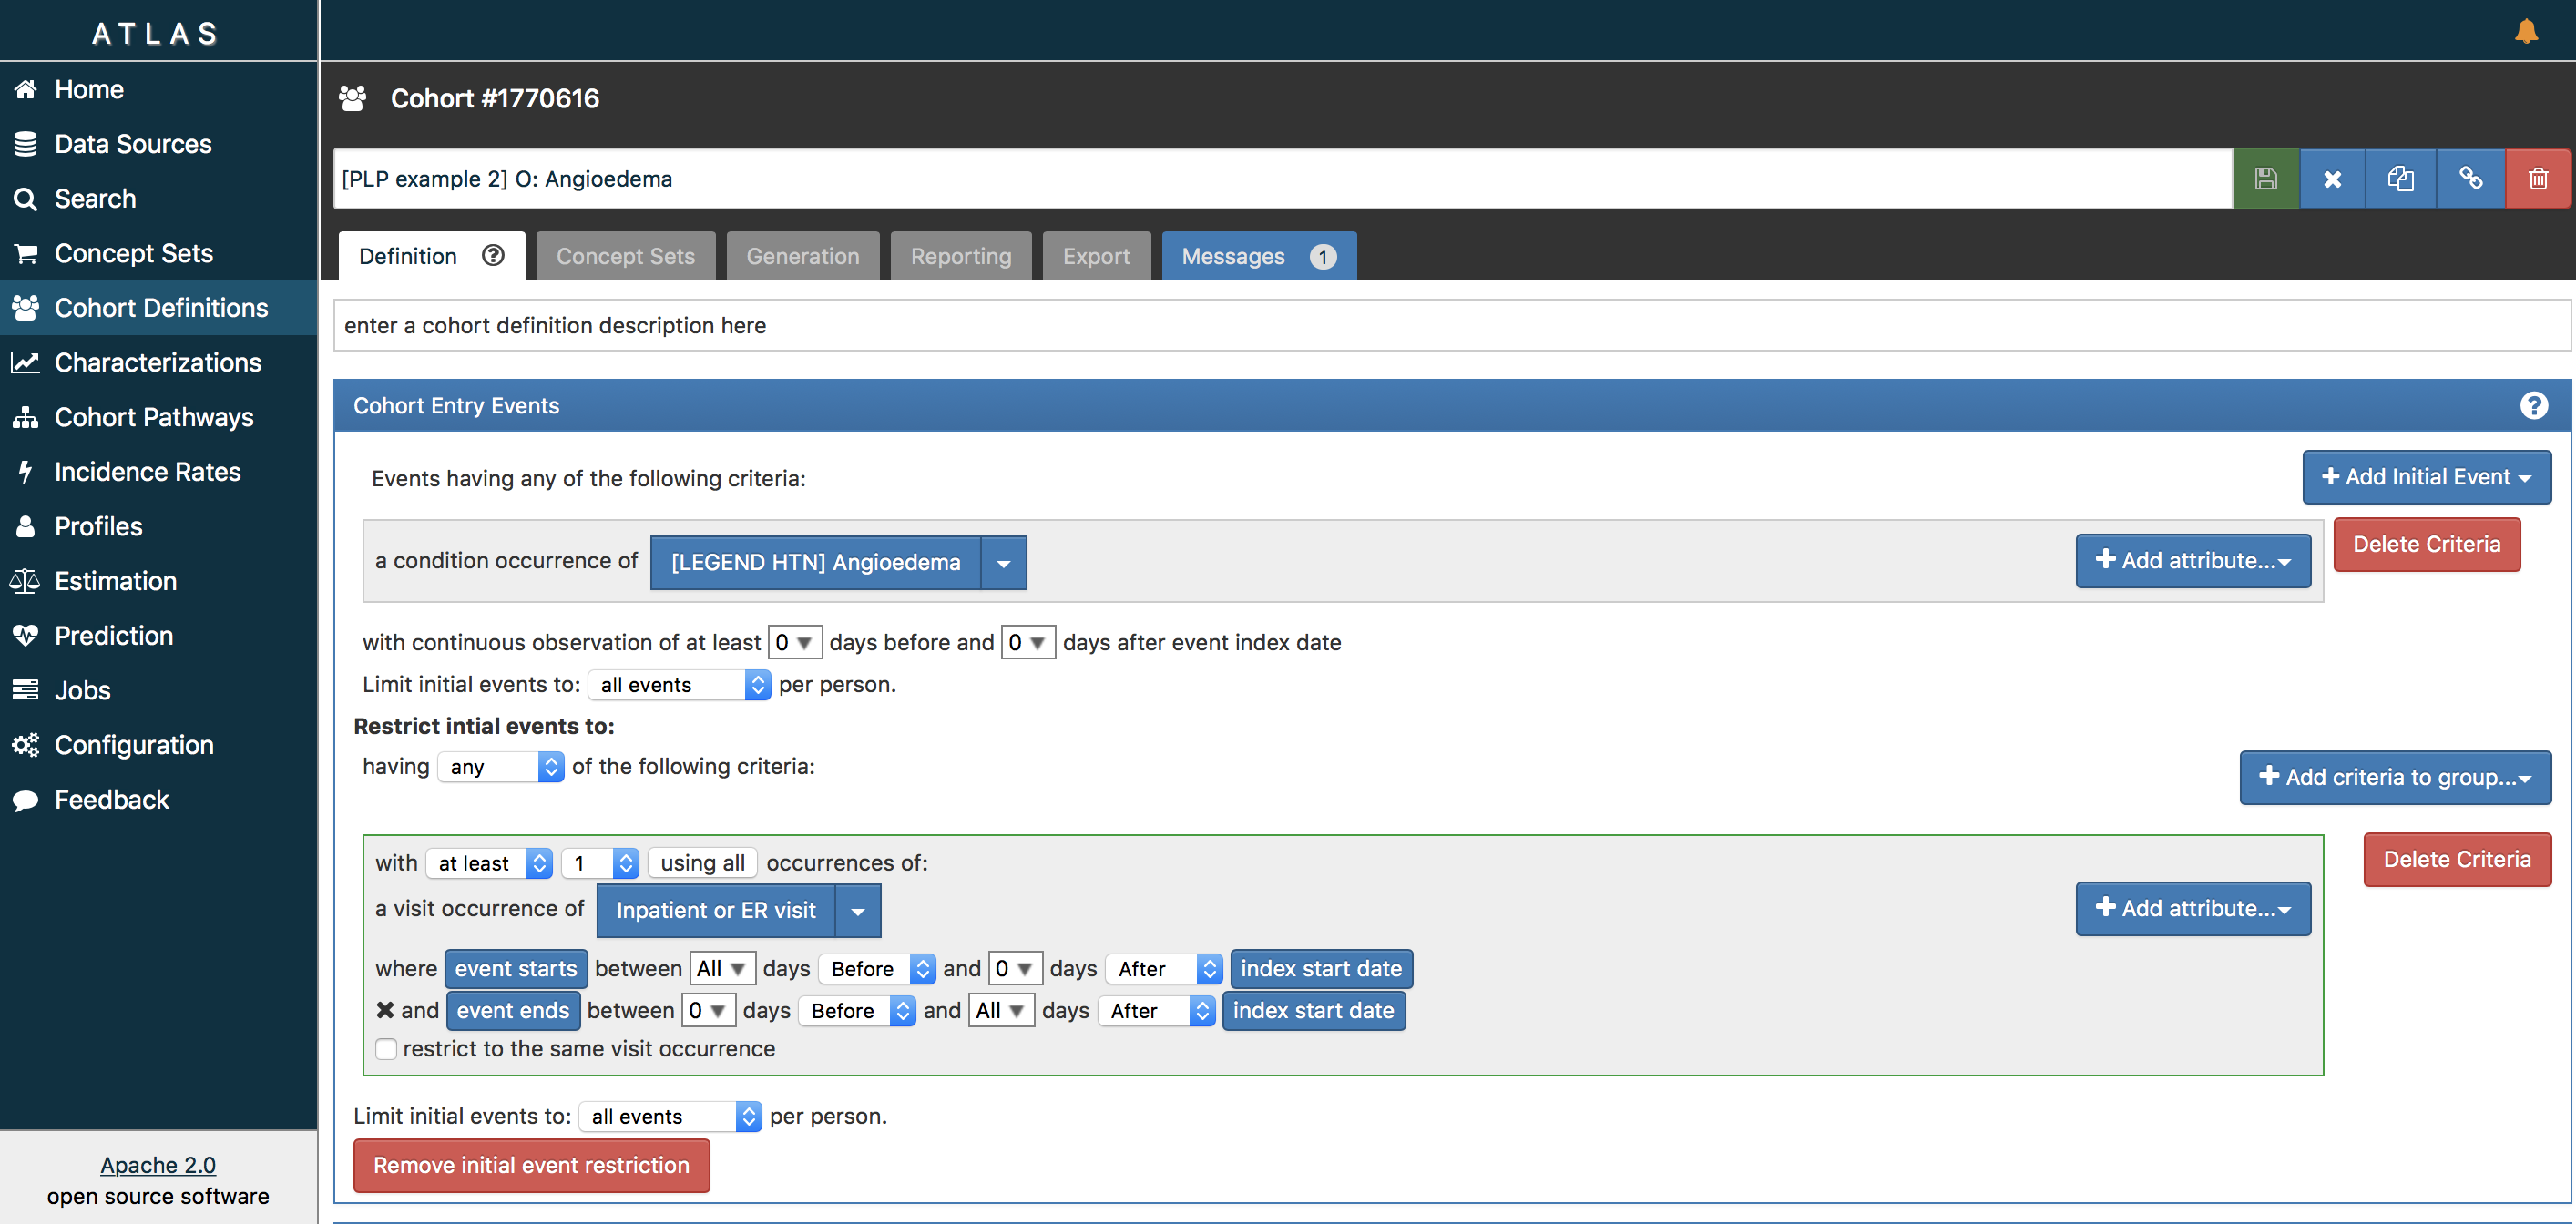
\includegraphics{example2/angioedema.png}
\caption{Outcome Cohort Angioedema}
\end{figure}

The T and O cohorts can be found here:

\begin{itemize}
\tightlist
\item
  Ace inhibitors (T):
  \url{http://www.ohdsi.org/web/atlas/\#/cohortdefinition/1770617}
\item
  Angioedema (O) :
  \url{http://www.ohdsi.org/web/atlas/\#/cohortdefinition/1770616}
\end{itemize}

In depth explanation of cohort creation in ATLAS is out of scope of this
vignette but can be found on the OHDSI wiki pages
\href{http://www.ohdsi.org/web/wiki/doku.php?id=documentation:software:atlas}{(link)}.

Note that when a cohort is created in ATLAS the cohortid is needed to
extract the data in R. The cohortid can be found at the top of the ATLAS
screen, e.g.~1770617 in Figure 6.

\hypertarget{custom-cohorts-1}{%
\subsubsection{Custom cohorts}\label{custom-cohorts-1}}

It is also possible to create cohorts without the use of ATLAS. Using
custom cohort code (SQL) you can make more advanced cohorts if needed.

For our example study, we need to create at table to hold the cohort
data and we need to create SQL code to instantiate this table for both
the AF and Stroke cohorts. Therefore, we create a file called
\emph{AceAngioCohorts.sql} with the following contents:

\begin{Shaded}
\begin{Highlighting}[]
  \CommentTok{/***********************************}
\CommentTok{    File AceAngioCohorts.sql }
\CommentTok{  ***********************************/}
    \CommentTok{/*}
\CommentTok{    Create a table to store the persons in the T and C cohort}
\CommentTok{  */}
    
    \ControlFlowTok{IF}\NormalTok{ OBJECT_ID(}\StringTok{'@resultsDatabaseSchema.PLPAceAngioCohort'}\NormalTok{, }\StringTok{'U'}\NormalTok{) }\KeywordTok{IS} \KeywordTok{NOT} \KeywordTok{NULL} 
  \KeywordTok{DROP} \KeywordTok{TABLE}\NormalTok{ @resultsDatabaseSchema.PLPAceAngioCohort;}
  
  \KeywordTok{CREATE} \KeywordTok{TABLE}\NormalTok{ @resultsDatabaseSchema.PLPAceAngioCohort }
\NormalTok{  ( }
\NormalTok{    cohort_definition_id }\DataTypeTok{INT}\NormalTok{, }
\NormalTok{    subject_id BIGINT,}
\NormalTok{    cohort_start_date }\DataTypeTok{DATE}\NormalTok{, }
\NormalTok{    cohort_end_date }\DataTypeTok{DATE}
\NormalTok{  );}
  
  
  \CommentTok{/*}
\CommentTok{    T cohort:  [PatientLevelPrediction vignette]:  T : patients who are newly }
\CommentTok{  dispensed an ACE inhibitor}
\CommentTok{  - persons with a drug exposure record of any 'ACE inhibitor' or }
\CommentTok{  any descendants, indexed at the first diagnosis}
\CommentTok{  - who have >364 days of prior observation before their first dispensing}
\CommentTok{  */}
    \KeywordTok{INSERT} \KeywordTok{INTO}\NormalTok{ @resultsDatabaseSchema.AceAngioCohort (cohort_definition_id, }
\NormalTok{                                                       subject_id, }
\NormalTok{                                                       cohort_start_date, }
\NormalTok{                                                       cohort_end_date)}
  \KeywordTok{SELECT} \DecValTok{1} \KeywordTok{AS}\NormalTok{ cohort_definition_id,}
\NormalTok{  Ace.person_id }\KeywordTok{AS}\NormalTok{ subject_id,}
\NormalTok{  Ace.drug_start_date }\KeywordTok{AS}\NormalTok{ cohort_start_date,}
\NormalTok{  observation_period.observation_period_end_date }\KeywordTok{AS}\NormalTok{ cohort_end_date}
  \KeywordTok{FROM}
\NormalTok{  (}
    \KeywordTok{SELECT}\NormalTok{ person_id, }\FunctionTok{min}\NormalTok{(drug_exposure_date) }\KeywordTok{as}\NormalTok{ drug_start_date}
    \KeywordTok{FROM}\NormalTok{ @cdmDatabaseSchema.drug_exposure}
    \KeywordTok{WHERE}\NormalTok{ drug_concept_id }\KeywordTok{IN}\NormalTok{ (}\KeywordTok{SELECT}\NormalTok{ descendant_concept_id }\KeywordTok{FROM} 
\NormalTok{                              @cdmDatabaseSchema.concept_ancestor }\KeywordTok{WHERE}\NormalTok{ ancestor_concept_id }\KeywordTok{IN} 
\NormalTok{                              (}\DecValTok{1342439}\NormalTok{,}\DecValTok{1334456}\NormalTok{, }\DecValTok{1331235}\NormalTok{, }\DecValTok{1373225}\NormalTok{, }\DecValTok{1310756}\NormalTok{, }\DecValTok{1308216}\NormalTok{, }\DecValTok{1363749}\NormalTok{, }\DecValTok{1341927}\NormalTok{, }\DecValTok{1340128}\NormalTok{, }\DecValTok{1335471} \CommentTok{/*ace inhibitors*/}\NormalTok{))}
    \KeywordTok{GROUP} \KeywordTok{BY}\NormalTok{ person_id}
\NormalTok{  ) Ace}
  \KeywordTok{INNER} \KeywordTok{JOIN}\NormalTok{ @cdmDatabaseSchema.observation_period}
  \KeywordTok{ON}\NormalTok{ Ace.person_id }\OperatorTok{=}\NormalTok{ observation_period.person_id}
  \KeywordTok{AND}\NormalTok{ Ace.drug_start_date }\OperatorTok{>=}\NormalTok{ dateadd(dd,}\DecValTok{364}\NormalTok{, }
\NormalTok{                                     observation_period.observation_period_start_date)}
  \KeywordTok{AND}\NormalTok{ Ace.drug_start_date }\OperatorTok{<=}\NormalTok{ observation_period.observation_period_end_date}
\NormalTok{  ;}
  
  \CommentTok{/*}
\CommentTok{    C cohort:  [PatientLevelPrediction vignette]:  O: Angioedema}
\CommentTok{  */}
    \KeywordTok{INSERT} \KeywordTok{INTO}\NormalTok{ @resultsDatabaseSchema.AceAngioCohort (cohort_definition_id, }
\NormalTok{                                                       subject_id, }
\NormalTok{                                                       cohort_start_date, }
\NormalTok{                                                       cohort_end_date)}
  \KeywordTok{SELECT} \DecValTok{2} \KeywordTok{AS}\NormalTok{ cohort_definition_id,}
\NormalTok{  angioedema.person_id }\KeywordTok{AS}\NormalTok{ subject_id,}
\NormalTok{  angioedema.condition_start_date }\KeywordTok{AS}\NormalTok{ cohort_start_date,}
\NormalTok{  angioedema.condition_start_date }\KeywordTok{AS}\NormalTok{ cohort_end_date}
  \KeywordTok{FROM}  
\NormalTok{  (}
    \KeywordTok{SELECT}\NormalTok{ person_id, condition_start_date}
    \KeywordTok{FROM}\NormalTok{ @cdmDatabaseSchema.condition_occurrence}
    \KeywordTok{WHERE}\NormalTok{ condition_concept_id }\KeywordTok{IN}\NormalTok{ (}\KeywordTok{SELECT} \KeywordTok{DISTINCT}\NormalTok{ descendant_concept_id }\KeywordTok{FROM} 
\NormalTok{                                   @cdmDatabaseSchema.concept_ancestor }\KeywordTok{WHERE}\NormalTok{ ancestor_concept_id }\KeywordTok{IN} 
\NormalTok{                                   (}\DecValTok{432791} \CommentTok{/*angioedema*/}\NormalTok{) }\KeywordTok{OR}\NormalTok{ descendant_concept_id }\KeywordTok{IN} 
\NormalTok{                                   (}\DecValTok{432791} \CommentTok{/*angioedema*/}\NormalTok{)}
\NormalTok{    ) angioedema}
    
\NormalTok{    ;}
    
\end{Highlighting}
\end{Shaded}

This is parameterized SQL which can be used by the
\href{http://github.com/OHDSI/SqlRender}{\texttt{SqlRender}} package. We
use parameterized SQL so we do not have to pre-specify the names of the
CDM and result schemas. That way, if we want to run the SQL on a
different schema, we only need to change the parameter values; we do not
have to change the SQL code. By also making use of translation
functionality in \texttt{SqlRender}, we can make sure the SQL code can
be run in many different environments.

To execute this sql against our CDM we first need to tell R how to
connect to the server. \texttt{PatientLevelPrediction} uses the
\href{http://github.com/ohdsi/DatabaseConnector}{\texttt{DatabaseConnector}}
package, which provides a function called
\texttt{createConnectionDetails}. Type \texttt{?createConnectionDetails}
for the specific settings required for the various database management
systems (DBMS). For example, one might connect to a PostgreSQL database
using this code:

\begin{Shaded}
\begin{Highlighting}[]
\NormalTok{    connectionDetails <-}\StringTok{ }\KeywordTok{createConnectionDetails}\NormalTok{(}\DataTypeTok{dbms =} \StringTok{"postgresql"}\NormalTok{, }
                                                 \DataTypeTok{server =} \StringTok{"localhost/ohdsi"}\NormalTok{, }
                                                 \DataTypeTok{user =} \StringTok{"joe"}\NormalTok{, }
                                                 \DataTypeTok{password =} \StringTok{"supersecret"}\NormalTok{)}
    
\NormalTok{    cdmDatabaseSchema <-}\StringTok{ "my_cdm_data"}
\NormalTok{    cohortsDatabaseSchema <-}\StringTok{ "my_results"}
\NormalTok{    cdmVersion <-}\StringTok{ "5"}
\end{Highlighting}
\end{Shaded}

The last three lines define the \texttt{cdmDatabaseSchema} and
\texttt{cohortsDatabaseSchema} variables, as well as the CDM version. We
will use these later to tell R where the data in CDM format live, where
we want to create the cohorts of interest, and what version CDM is used.
Note that for Microsoft SQL Server, databaseschemas need to specify both
the database and the schema, so for example
\texttt{cdmDatabaseSchema\ \textless{}-\ "my\_cdm\_data.dbo"}.

\begin{Shaded}
\begin{Highlighting}[]
    \KeywordTok{library}\NormalTok{(SqlRender)}
\NormalTok{    sql <-}\StringTok{ }\KeywordTok{readSql}\NormalTok{(}\StringTok{"AceAngioCohorts.sql"}\NormalTok{)}
\NormalTok{    sql <-}\StringTok{ }\KeywordTok{render}\NormalTok{(sql,}
                  \DataTypeTok{cdmDatabaseSchema =}\NormalTok{ cdmDatabaseSchema,}
                  \DataTypeTok{cohortsDatabaseSchema =}\NormalTok{ cohortsDatabaseSchema)}
\NormalTok{    sql <-}\StringTok{ }\KeywordTok{translate}\NormalTok{(sql, }\DataTypeTok{targetDialect =}\NormalTok{ connectionDetails}\OperatorTok{$}\NormalTok{dbms)}
    
\NormalTok{    connection <-}\StringTok{ }\KeywordTok{connect}\NormalTok{(connectionDetails)}
    \KeywordTok{executeSql}\NormalTok{(connection, sql)}
\end{Highlighting}
\end{Shaded}

In this code, we first read the SQL from the file into memory. In the
next line, we replace four parameter names with the actual values. We
then translate the SQL into the dialect appropriate for the DBMS we
already specified in the \texttt{connectionDetails}. Next, we connect to
the server, and submit the rendered and translated SQL.

If all went well, we now have a table with the events of interest. We
can see how many events per type:

\begin{Shaded}
\begin{Highlighting}[]
\NormalTok{    sql <-}\StringTok{ }\KeywordTok{paste}\NormalTok{(}\StringTok{"SELECT cohort_definition_id, COUNT(*) AS count"}\NormalTok{,}
                 \StringTok{"FROM @cohortsDatabaseSchema.AceAngioCohort"}\NormalTok{,}
                 \StringTok{"GROUP BY cohort_definition_id"}\NormalTok{)}
\NormalTok{    sql <-}\StringTok{ }\KeywordTok{render}\NormalTok{(sql, }\DataTypeTok{cohortsDatabaseSchema =}\NormalTok{ cohortsDatabaseSchema)}
\NormalTok{    sql <-}\StringTok{ }\KeywordTok{translate}\NormalTok{(sql, }\DataTypeTok{targetDialect =}\NormalTok{ connectionDetails}\OperatorTok{$}\NormalTok{dbms)}
    
    \KeywordTok{querySql}\NormalTok{(connection, sql)}
\end{Highlighting}
\end{Shaded}

\begin{verbatim}
##   cohort_definition_id count
## 1                    1     0
## 2                    2     0
\end{verbatim}

\hypertarget{study-script-creation-1}{%
\subsubsection{Study script creation}\label{study-script-creation-1}}

In this section we assume that our cohorts have been created either by
using ATLAS or a custom SQL script. We will first explain how to create
an R script yourself that will execute our study as we have defined
earlier.

\hypertarget{data-extraction-1}{%
\subsubsection{Data extraction}\label{data-extraction-1}}

Now we can tell \texttt{PatientLevelPrediction} to extract all necessary
data for our analysis. This is done using the
\href{https://github.com/OHDSI/FeatureExtration}{\texttt{FeatureExtractionPackage}}.
In short the FeatureExtractionPackage allows you to specify which
features (covariates) need to be extracted, e.g.~all conditions and drug
exposures. It also supports the creation of custom covariates. For more
detailed information on the FeatureExtraction package see its
\href{https://github.com/OHDSI/FeatureExtration}{vignettes}. For our
example study we decided to use these settings:

\begin{Shaded}
\begin{Highlighting}[]
\NormalTok{    covariateSettings <-}\StringTok{ }\KeywordTok{createCovariateSettings}\NormalTok{(}\DataTypeTok{useDemographicsGender =} \OtherTok{TRUE}\NormalTok{,}
                                                 \DataTypeTok{useDemographicsAge =} \OtherTok{TRUE}\NormalTok{,}
                                                 \DataTypeTok{useConditionGroupEraLongTerm =} \OtherTok{TRUE}\NormalTok{,}
                                                 \DataTypeTok{useConditionGroupEraAnyTimePrior =} \OtherTok{TRUE}\NormalTok{,}
                                                 \DataTypeTok{useDrugGroupEraLongTerm =} \OtherTok{TRUE}\NormalTok{,}
                                                 \DataTypeTok{useDrugGroupEraAnyTimePrior =} \OtherTok{TRUE}\NormalTok{,}
                                                 \DataTypeTok{useVisitConceptCountLongTerm =} \OtherTok{TRUE}\NormalTok{,}
                                                 \DataTypeTok{longTermStartDays =} \DecValTok{-365}\NormalTok{,}
                                                 \DataTypeTok{endDays =} \DecValTok{-1}\NormalTok{)}
\end{Highlighting}
\end{Shaded}

The final step for extracting the data is to run the \texttt{getPlpData}
function and input the connection details, the database schema where the
cohorts are stored, the cohort definition ids for the cohort and
outcome, and the washoutPeriod which is the minimum number of days prior
to cohort index date that the person must have been observed to be
included into the data, and finally input the previously constructed
covariate settings.

\begin{Shaded}
\begin{Highlighting}[]
\NormalTok{    plpData <-}\StringTok{ }\KeywordTok{getPlpData}\NormalTok{(}\DataTypeTok{connectionDetails =}\NormalTok{ connectionDetails,}
                          \DataTypeTok{cdmDatabaseSchema =}\NormalTok{ cdmDatabaseSchema,}
                          \DataTypeTok{cohortDatabaseSchema =}\NormalTok{ resultsDatabaseSchema,}
                          \DataTypeTok{cohortTable =} \StringTok{'AceAngioCohort'}\NormalTok{,}
                          \DataTypeTok{cohortId =} \DecValTok{1}\NormalTok{,}
                          \DataTypeTok{covariateSettings =}\NormalTok{ covariateSettings,}
                          \DataTypeTok{outcomeDatabaseSchema =}\NormalTok{ resultsDatabaseSchema,}
                          \DataTypeTok{outcomeTable =} \StringTok{'AceAngioCohort'}\NormalTok{,}
                          \DataTypeTok{outcomeIds =} \DecValTok{2}\NormalTok{,}
                          \DataTypeTok{sampleSize =} \DecValTok{10000}
\NormalTok{    )}
\end{Highlighting}
\end{Shaded}

Note that if the cohorts are created in ATLAS its corresponding cohort
database schema needs to be selected. There are many additional
parameters for the \texttt{getPlpData} function which are all documented
in the \texttt{PatientLevelPrediction} manual. The resulting
\texttt{plpData} object uses the package \texttt{ff} to store
information in a way that ensures R does not run out of memory, even
when the data are large.

Creating the \texttt{plpData} object can take considerable computing
time, and it is probably a good idea to save it for future sessions.
Because \texttt{plpData} uses \texttt{ff}, we cannot use R's regular
save function. Instead, we'll have to use the \texttt{savePlpData()}
function:

\begin{Shaded}
\begin{Highlighting}[]
\KeywordTok{savePlpData}\NormalTok{(plpData, }\StringTok{"angio_in_ace_data"}\NormalTok{)}
\end{Highlighting}
\end{Shaded}

We can use the \texttt{loadPlpData()} function to load the data in a
future session.

\hypertarget{additional-inclusion-criteria-1}{%
\subsubsection{Additional inclusion
criteria}\label{additional-inclusion-criteria-1}}

To completely define the prediction problem the final study population
is obtained by applying additional constraints on the two earlier
defined cohorts, e.g., a minumim time at risk can be enforced
(\texttt{requireTimeAtRisk,\ minTimeAtRisk}) and we can specify if this
also applies to patients with the outcome (\texttt{includeAllOutcomes}).
Here we also specify the start and end of the risk window relative to
target cohort start. For example, if we like the risk window to start 30
days after the at-risk cohort start and end a year later we can set
\texttt{riskWindowStart\ =\ 30} and \texttt{riskWindowEnd\ =\ 365}. In
some cases the risk window needs to start at the cohort end date. This
can be achieved by setting \texttt{addExposureToStart\ =\ TRUE} which
adds the cohort (exposure) time to the start date.

In Appendix 1, we demonstrate the effect of these settings on the subset
of the persons in the target cohort that end up in the final study
population.

In the example below all the settings we defined for our study are
imposed:

\begin{Shaded}
\begin{Highlighting}[]
\NormalTok{    population <-}\StringTok{ }\KeywordTok{createStudyPopulation}\NormalTok{(}\DataTypeTok{plpData =}\NormalTok{ plpData,}
                                        \DataTypeTok{outcomeId =} \DecValTok{2}\NormalTok{,}
                                        \DataTypeTok{washoutPeriod =} \DecValTok{364}\NormalTok{,}
                                        \DataTypeTok{firstExposureOnly =} \OtherTok{FALSE}\NormalTok{,}
                                        \DataTypeTok{removeSubjectsWithPriorOutcome =} \OtherTok{TRUE}\NormalTok{,}
                                        \DataTypeTok{priorOutcomeLookback =} \DecValTok{9999}\NormalTok{,}
                                        \DataTypeTok{riskWindowStart =} \DecValTok{1}\NormalTok{,}
                                        \DataTypeTok{riskWindowEnd =} \DecValTok{365}\NormalTok{,}
                                        \DataTypeTok{addExposureDaysToStart =} \OtherTok{FALSE}\NormalTok{,}
                                        \DataTypeTok{addExposureDaysToEnd =} \OtherTok{FALSE}\NormalTok{,}
                                        \DataTypeTok{minTimeAtRisk =} \DecValTok{364}\NormalTok{,}
                                        \DataTypeTok{requireTimeAtRisk =} \OtherTok{TRUE}\NormalTok{,}
                                        \DataTypeTok{includeAllOutcomes =} \OtherTok{TRUE}\NormalTok{,}
                                        \DataTypeTok{verbosity =} \StringTok{"DEBUG"}
\NormalTok{    )}
\end{Highlighting}
\end{Shaded}

\hypertarget{model-development-1}{%
\subsubsection{Model Development}\label{model-development-1}}

In the set function of an algorithm the user can specify a list of
eligible values for each hyper-parameter. All possible combinations of
the hyper-parameters are included in a so-called grid search using
cross-validation on the training set. If a user does not specify any
value then the default value is used instead.

For example, if we use the following settings for the
gradientBoostingMachine: ntrees=c(100,200), maxDepth=4 the grid search
will apply the gradient boosting machine algorithm with ntrees=100 and
maxDepth=4 plus the default settings for other hyper-parameters and
ntrees=200 and maxDepth=4 plus the default settings for other
hyper-parameters. The hyper-parameters that lead to the
bestcross-validation performance will then be chosen for the final
model. For our problem we choose to build a logistic regression model
with the default hyper-parameters

\begin{Shaded}
\begin{Highlighting}[]
\NormalTok{gbmModel <-}\StringTok{ }\KeywordTok{setGradientBoostingMachine}\NormalTok{(}\DataTypeTok{ntrees =} \DecValTok{5000}\NormalTok{, }\DataTypeTok{maxDepth =} \KeywordTok{c}\NormalTok{(}\DecValTok{4}\NormalTok{, }\DecValTok{7}\NormalTok{, }\DecValTok{10}\NormalTok{), }\DataTypeTok{learnRate =} \KeywordTok{c}\NormalTok{(}\FloatTok{0.001}\NormalTok{, }
    \FloatTok{0.01}\NormalTok{, }\FloatTok{0.1}\NormalTok{, }\FloatTok{0.9}\NormalTok{))}
\end{Highlighting}
\end{Shaded}

The \texttt{runPlP} function uses the population, \texttt{plpData}, and
model settings to train and evaluate the model. We can use the testSplit
(person/time) and testFraction parameters to split the data in a
75\%-25\% split and run the patient-level prediction pipeline:

\begin{Shaded}
\begin{Highlighting}[]
\NormalTok{    gbmResults <-}\StringTok{ }\KeywordTok{runPlp}\NormalTok{(population, plpData, }\DataTypeTok{modelSettings =}\NormalTok{ gbmModel, }\DataTypeTok{testSplit=}\StringTok{'stratified'}\NormalTok{, }
                         \DataTypeTok{testFraction=}\FloatTok{0.25}\NormalTok{, }\DataTypeTok{nfold=}\DecValTok{2}\NormalTok{, }\DataTypeTok{splitSeed =} \DecValTok{1234}\NormalTok{)}
\end{Highlighting}
\end{Shaded}

Under the hood the package will now use the R xgboost package to fit a a
gradient boosting machine model using 75\% of the data and will evaluate
the model on the remaining 25\%. A results data structure is returned
containing information about the model, its performance etc.

In the runPlp function there are several parameters to save the plpData,
plpResults, plpPlots, evaluation etc. which are all set to True by
default. However, there is also some functionality to this manually.

You can save the model using:

\begin{Shaded}
\begin{Highlighting}[]
\KeywordTok{savePlpModel}\NormalTok{(gbmResults}\OperatorTok{$}\NormalTok{model, }\DataTypeTok{dirPath =} \KeywordTok{file.path}\NormalTok{(}\KeywordTok{getwd}\NormalTok{(), }\StringTok{"model"}\NormalTok{))}
\end{Highlighting}
\end{Shaded}

You can load the model using:

\begin{Shaded}
\begin{Highlighting}[]
\NormalTok{plpModel <-}\StringTok{ }\KeywordTok{loadPlpModel}\NormalTok{(}\KeywordTok{file.path}\NormalTok{(}\KeywordTok{getwd}\NormalTok{(), }\StringTok{"model"}\NormalTok{))}
\end{Highlighting}
\end{Shaded}

You can also save the full results structure using:

\begin{Shaded}
\begin{Highlighting}[]
\KeywordTok{savePlpResult}\NormalTok{(gbmResults, }\DataTypeTok{location =} \KeywordTok{file.path}\NormalTok{(}\KeywordTok{getwd}\NormalTok{(), }\StringTok{"gbm"}\NormalTok{))}
\end{Highlighting}
\end{Shaded}

To load the full results structure use:

\begin{Shaded}
\begin{Highlighting}[]
\NormalTok{gbmResults <-}\StringTok{ }\KeywordTok{loadPlpResult}\NormalTok{(}\KeywordTok{file.path}\NormalTok{(}\KeywordTok{getwd}\NormalTok{(), }\StringTok{"gbm"}\NormalTok{))}
\end{Highlighting}
\end{Shaded}

\newpage

\hypertarget{study-package-creation}{%
\section{Study package creation}\label{study-package-creation}}

The script we created manually above can also be automatically created
using a powerful feature in ATLAS. By creating a new prediction study
(left menu) you can select the Target and Outcome as created in ATLAS,
set all the study parameters, and then you can download a R package that
you can use to execute your study. What is really powerful is that you
can add multiple Ts, Os, covariate settings etc. The package will then
run all the combinations of automatically as separate analyses. The
screenshots below explain this process.

\begin{enumerate}
\def\labelenumi{\arabic{enumi})}
\item
  Create a new prediction study and select your target and outcome
  cohorts.

  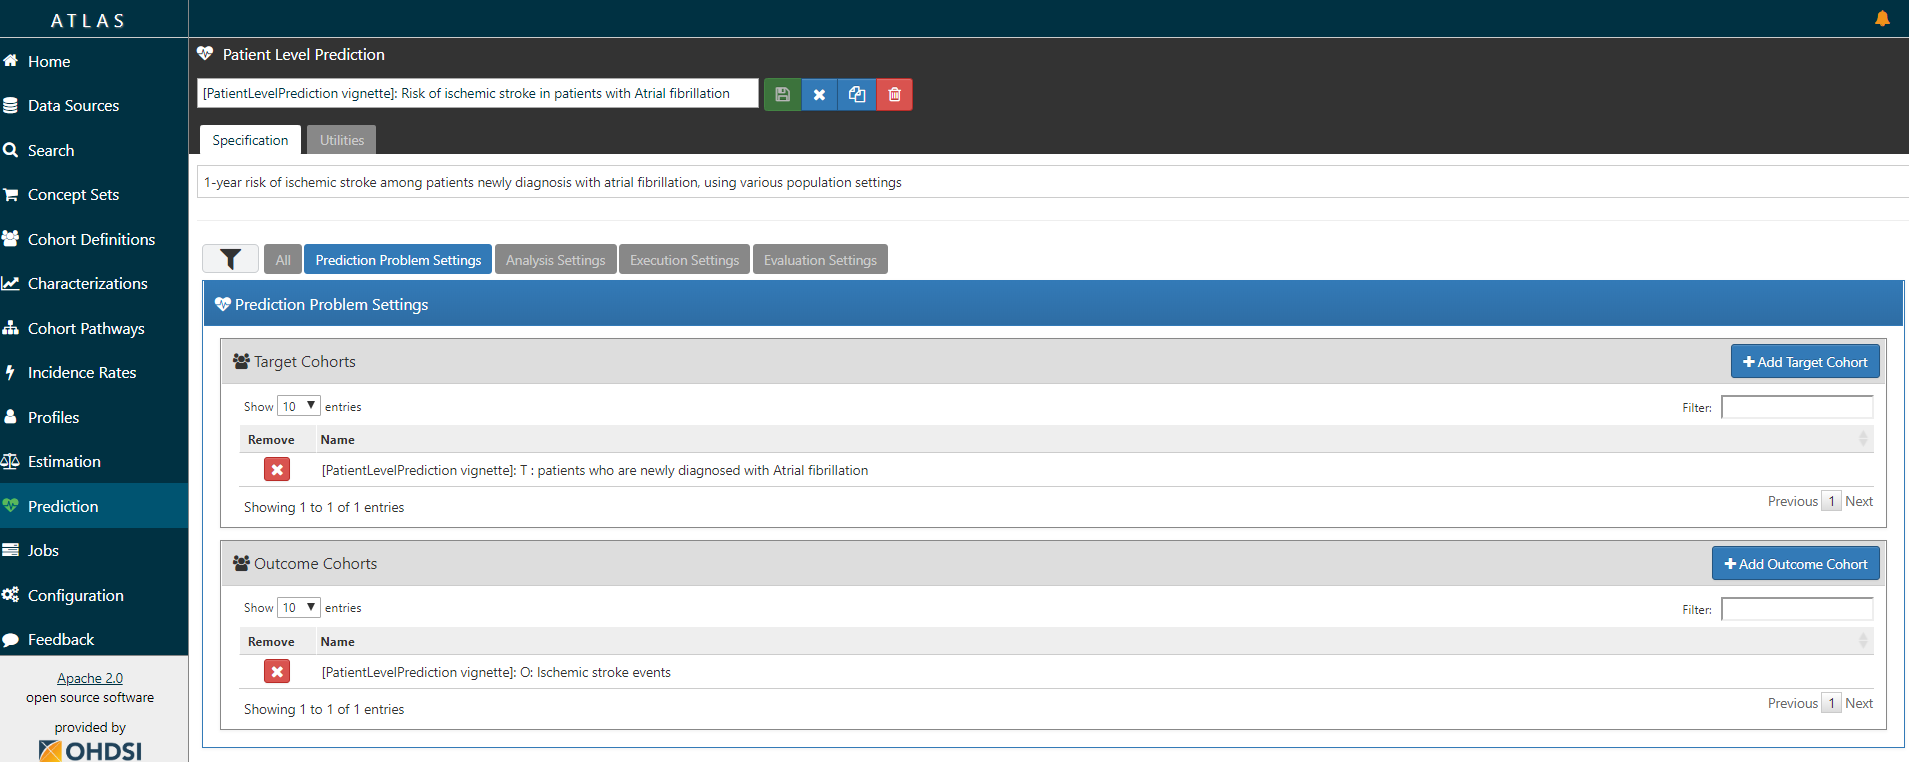
\includegraphics{atlasplp1.png}
\item
  Specify one or more analysis settings.

  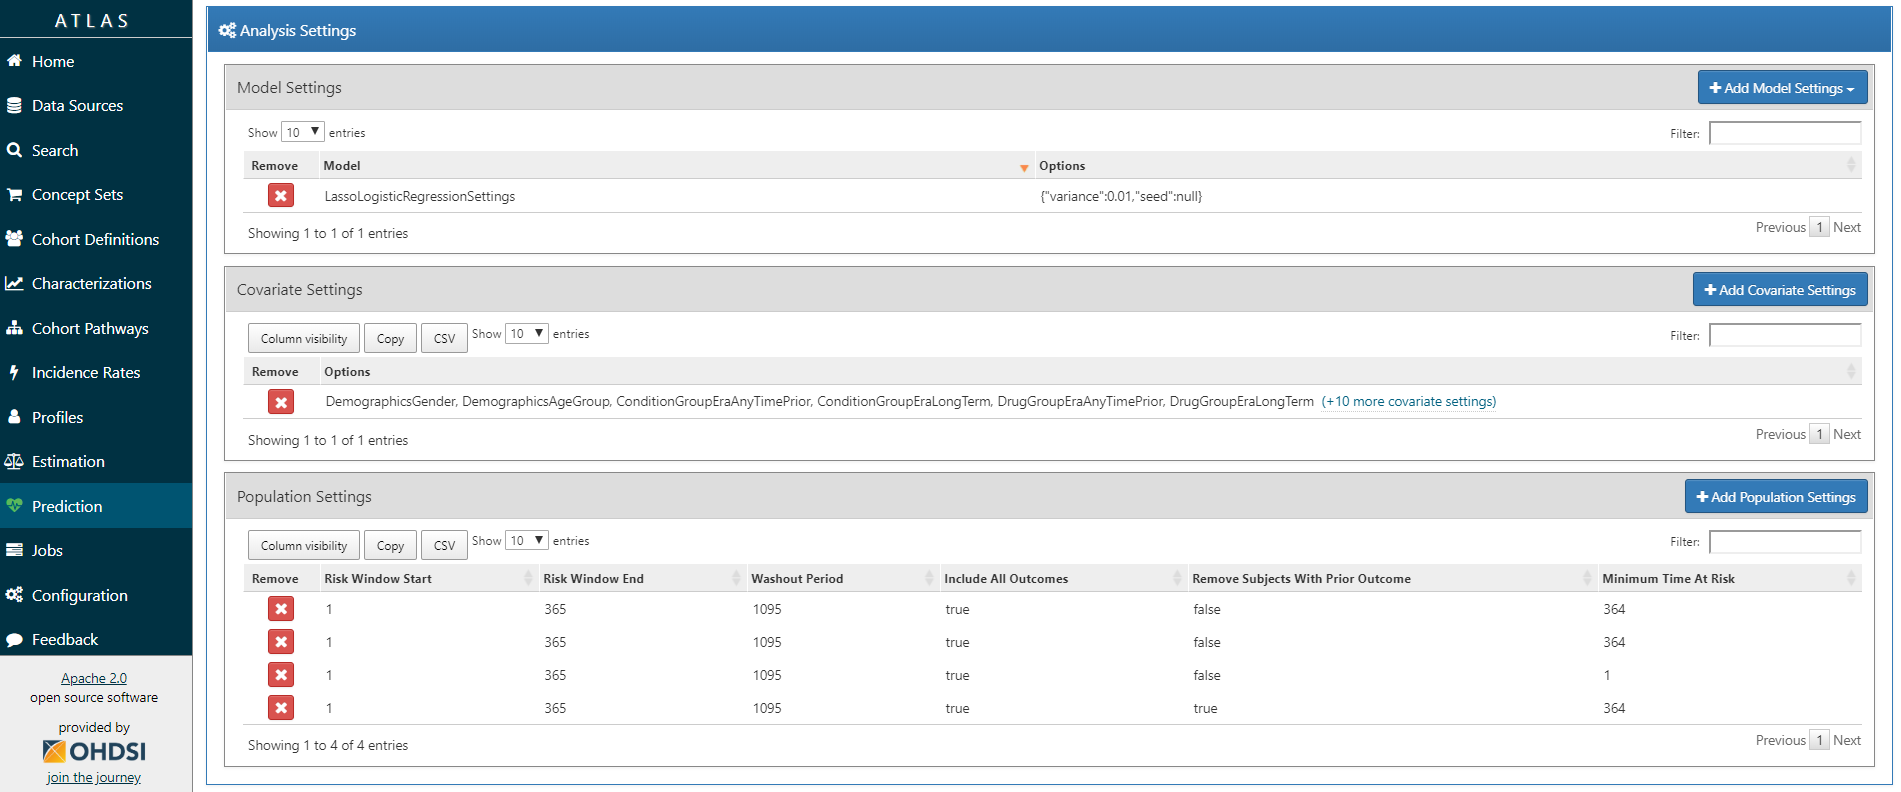
\includegraphics{atlasplp2.png}

  \newpage
\item
  Specify the trainings settigns

  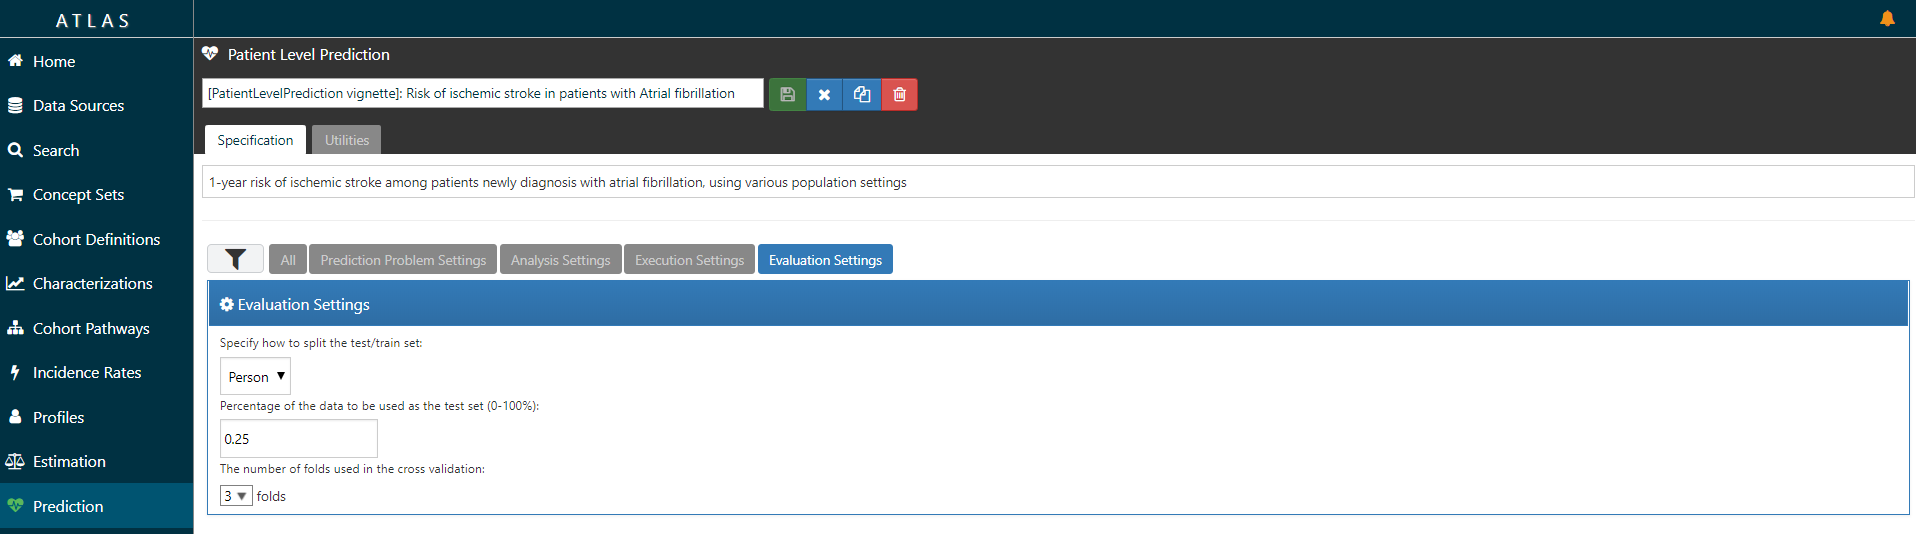
\includegraphics{atlasplp3.png}
\item
  Specify the execution settings

  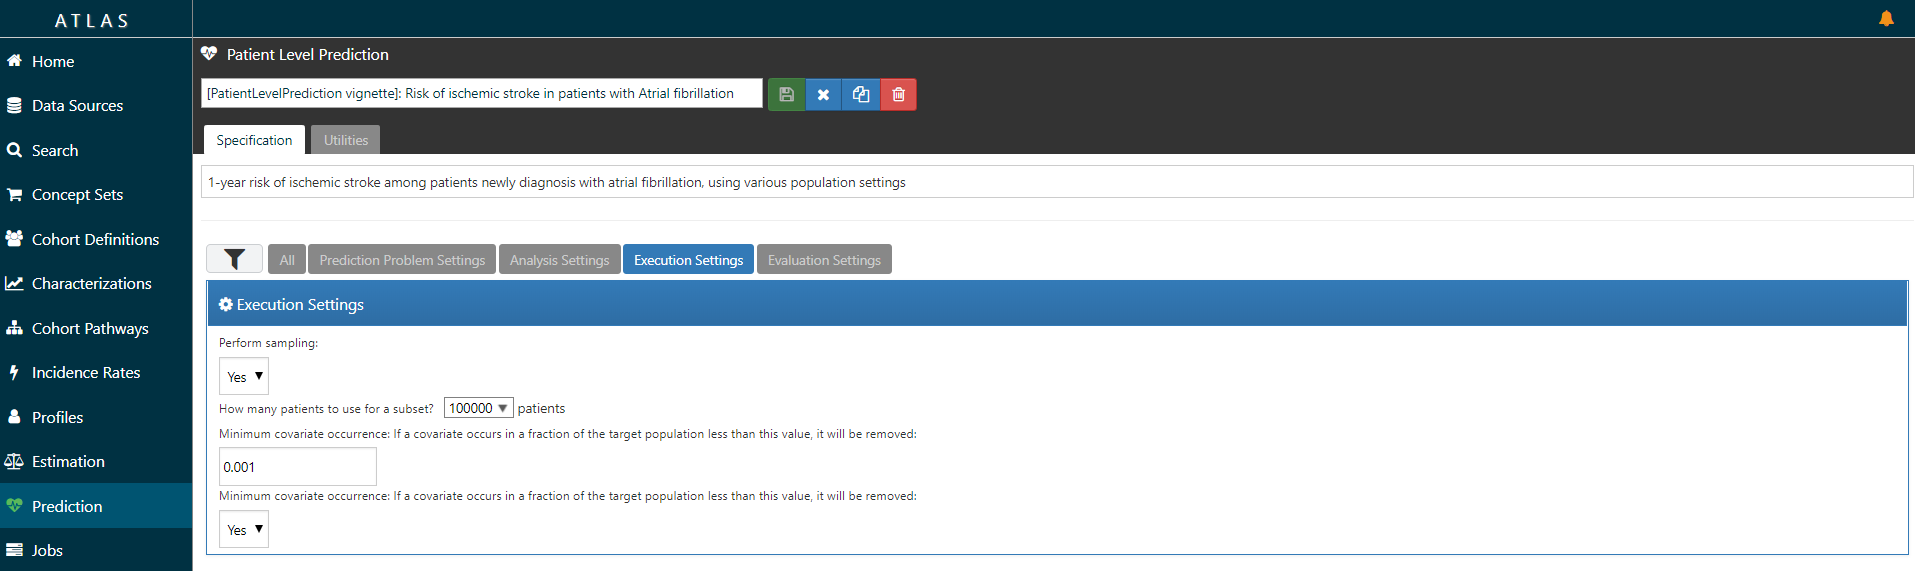
\includegraphics{atlasplp4.png}
\end{enumerate}

\newpage

ATLAS can build a R package for you that will execute the full study
against you CDM. Below the steps are explained how to do this in ATLAS.

\begin{enumerate}
\def\labelenumi{\arabic{enumi})}
\item
  Under utilities you can find download. Click on the button to review
  the full study specification

  \begin{figure}
  \centering
  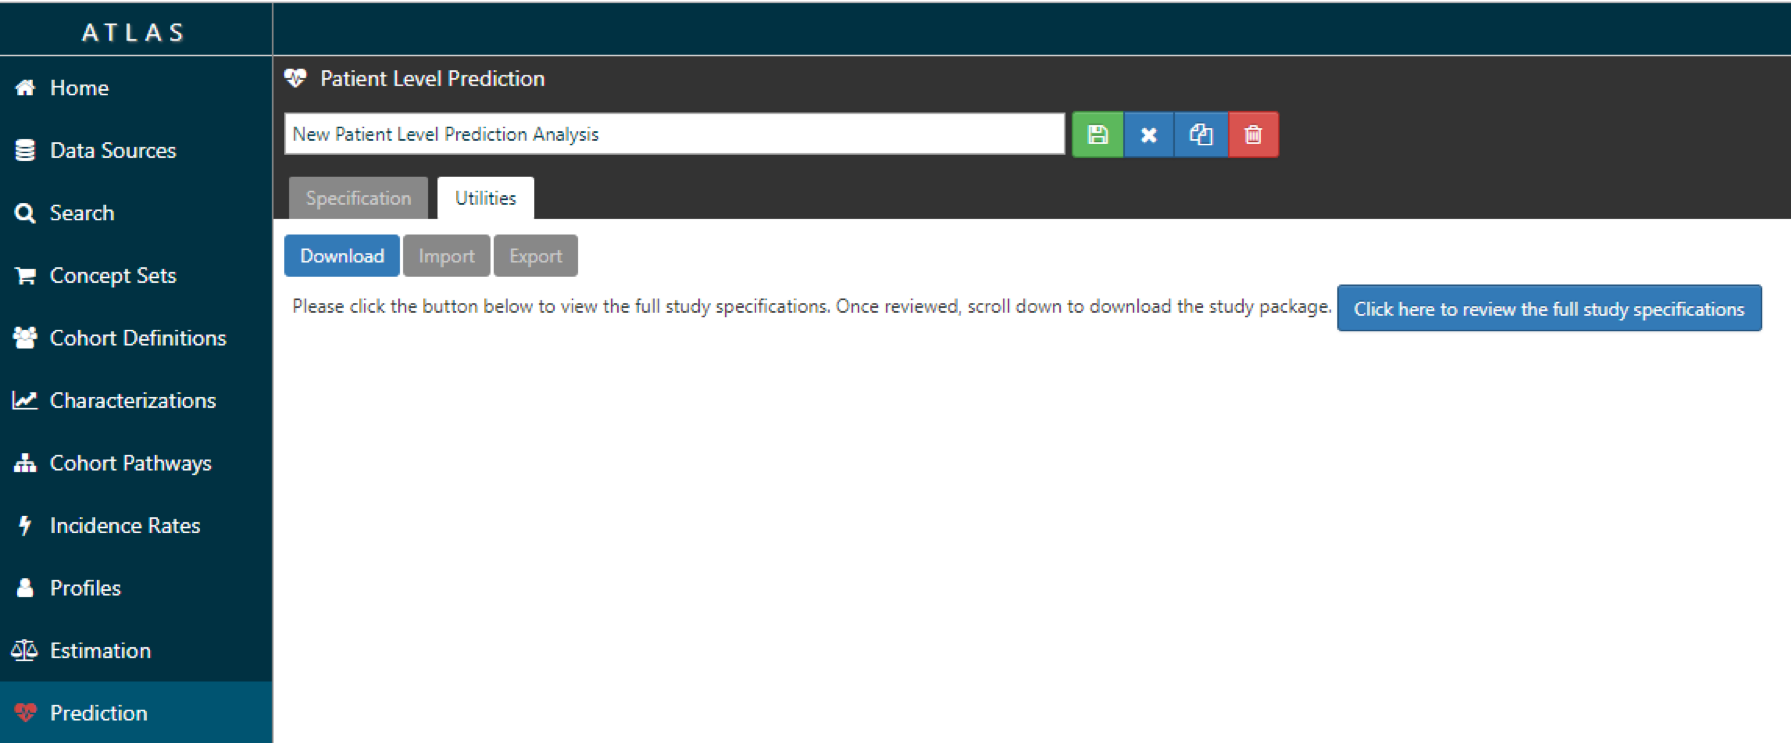
\includegraphics{atlasdownload1.png}
  \caption{R package download functionality in ATLAS}
  \end{figure}
\item
  You now have to review that you indeed want to run all these analyses
  (cartesian product of all the settings for each T and O combination.

  \begin{figure}
  \centering
  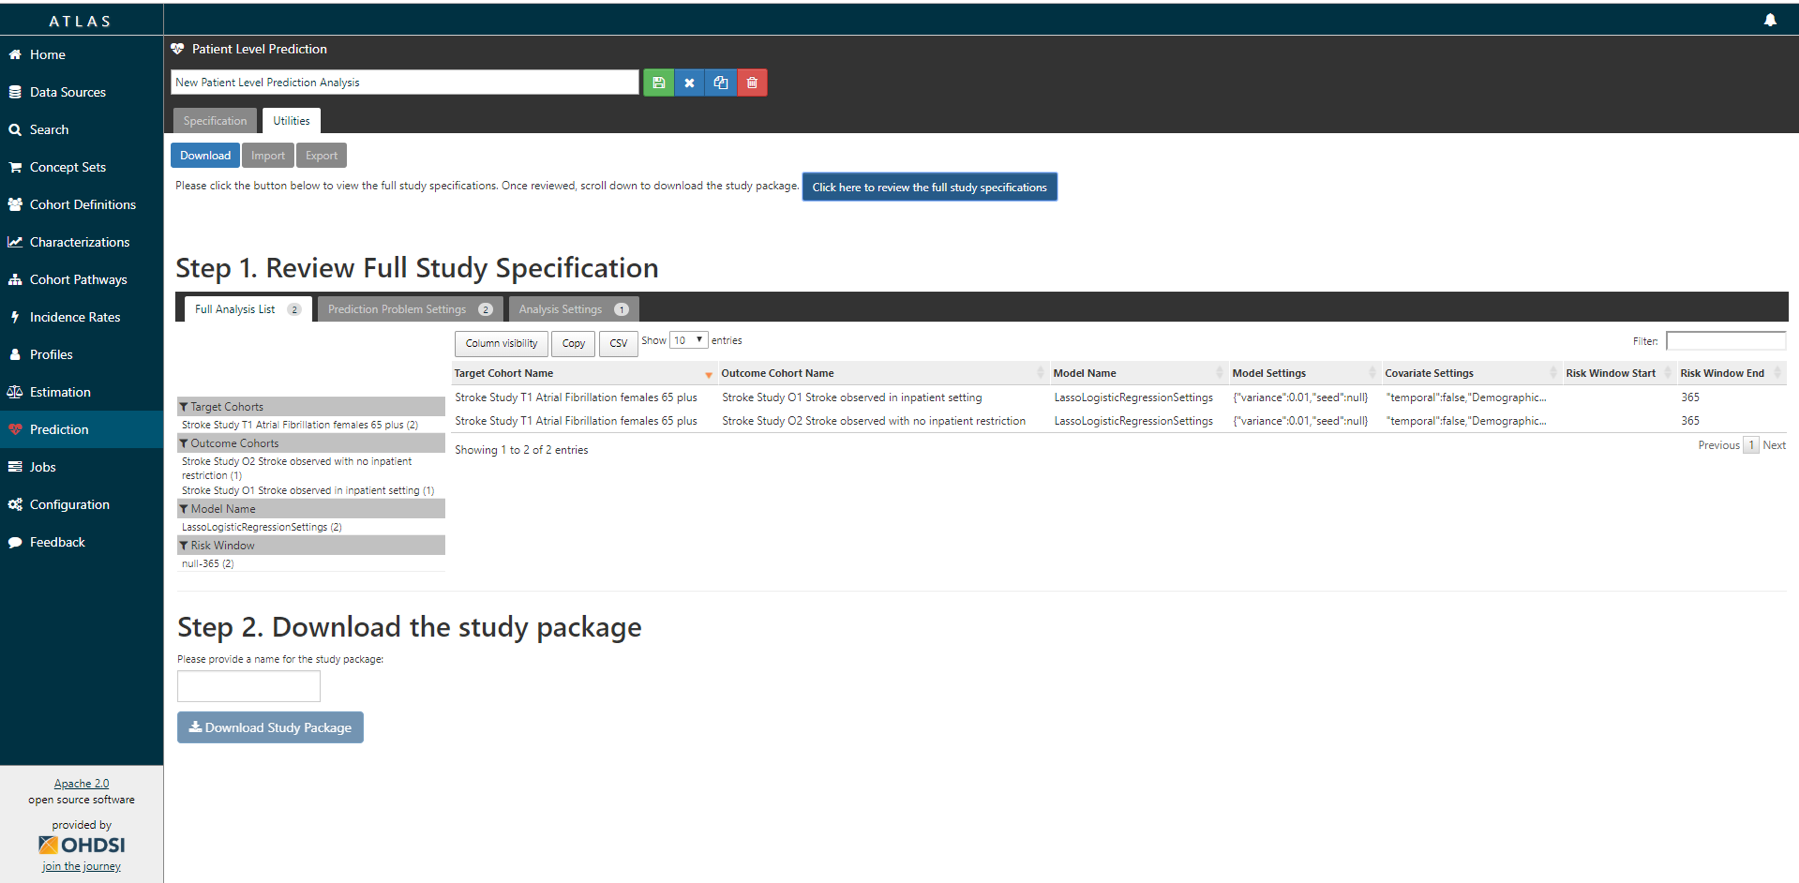
\includegraphics{atlasdownload2.png}
  \caption{R package download functionality in ATLAS}
  \end{figure}
\item
  If you agree, you give the package a name, and download the package as
  a zipfile.
\item
  By opening the R package in R studio and building the package you can
  run the study using the \texttt{execute} function. Theres is also an
  example CodeToRun.R script available in the extras folder of the
  package with extra instructions.
\end{enumerate}

\hypertarget{internal-validation}{%
\section{Internal validation}\label{internal-validation}}

Once we execute the study, the runPlp() function returns the trained
model and the evaluation of the model on the train/test sets.

You can interactively view the results by running:
\texttt{viewPlp(runPlp=lrResults)}. This will generate a Shiny App in
your browser in which you can view all performance measures created by
the framework as shown in the figure below.

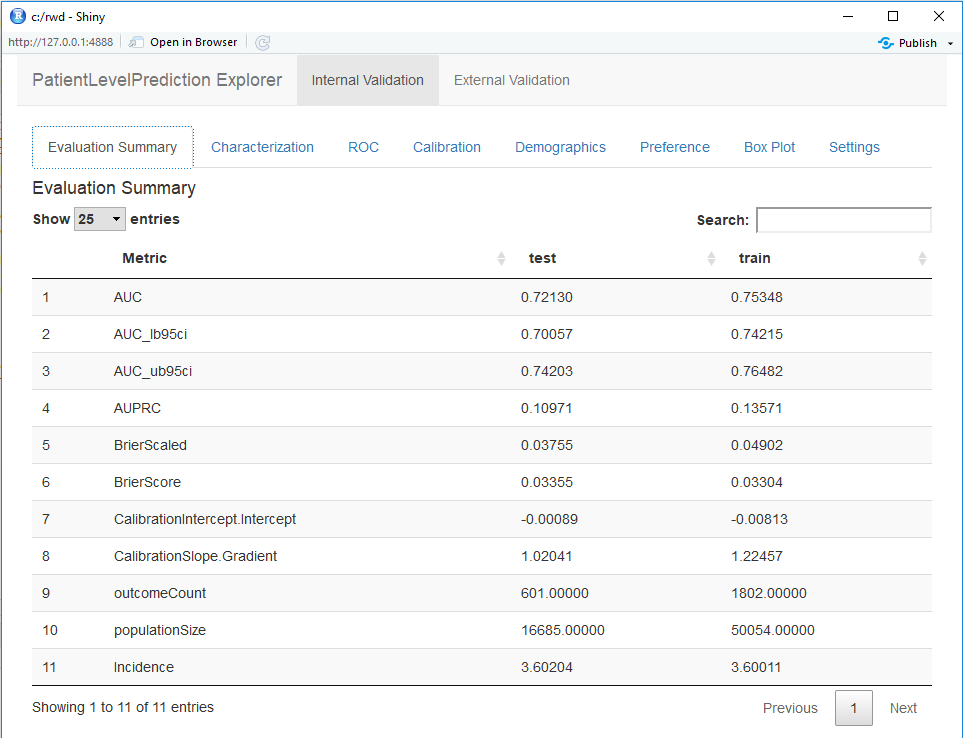
\includegraphics{shinysummary.png}

Furthermore, many interactive plots are available in the Shiny App, for
example the ROC curve in which you can move over the plot to see the
threshold and the corresponding sensitivity and specificity values.

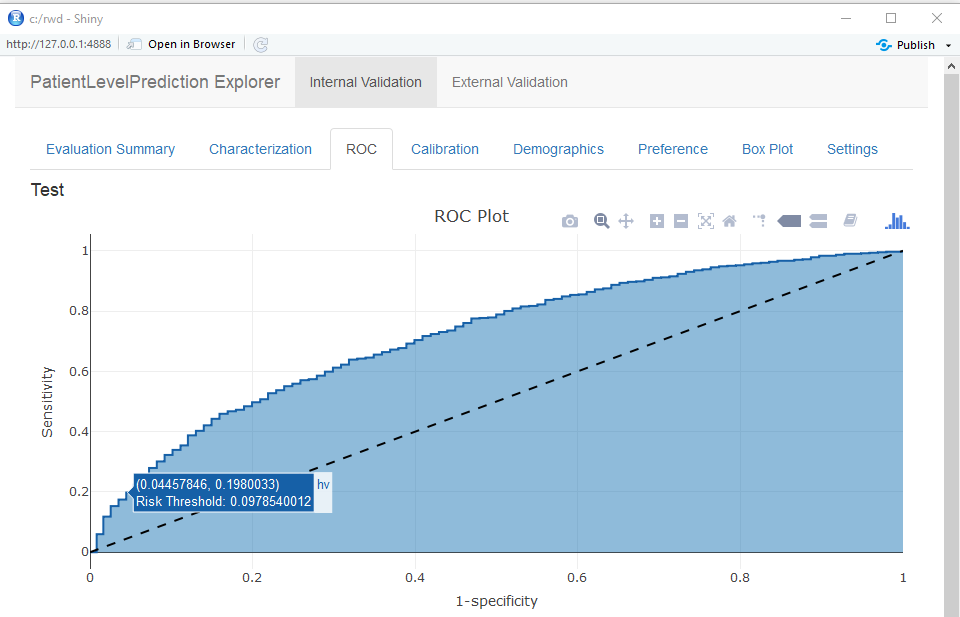
\includegraphics{shinyroc.png}

To generate and save all the evaluation plots to a folder run the
following code:

\begin{Shaded}
\begin{Highlighting}[]
\KeywordTok{plotPlp}\NormalTok{(lrResults, }\DataTypeTok{dirPath =} \KeywordTok{getwd}\NormalTok{())}
\end{Highlighting}
\end{Shaded}

The plots are described in more detail in the next sections.

\newpage

\hypertarget{discrimination}{%
\subsection{Discrimination}\label{discrimination}}

The Receiver Operating Characteristics (ROC) plot shows the sensitivity
against 1-specificity on the test set. The plot illustrates how well the
model is able to discriminate between the people with the outcome and
those without. The dashed diagonal line is the performance of a model
that randomly assigns predictions. The higher the area under the ROC
plot the better the discrimination of the model. The plot is created by
changing the probability threshold to assign the positive class.

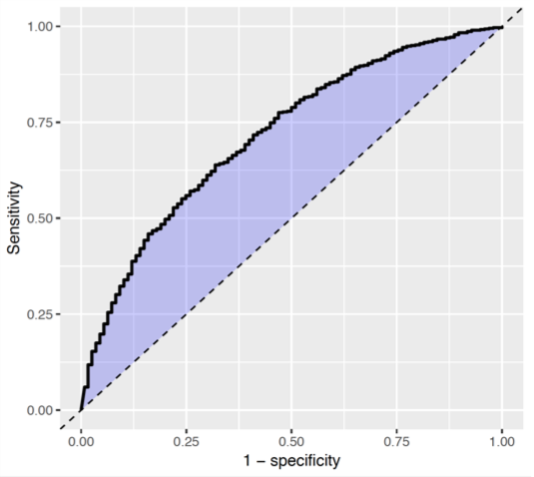
\includegraphics{sparseRoc.png}

\newpage \#\# Calibration

The calibration plot shows how close the predicted risk is to the
observed risk. The diagonal dashed line thus indicates a perfectly
calibrated model. The ten (or fewer) dots represent the mean predicted
values for each quantile plotted against the observed fraction of people
in that quantile who had the outcome (observed fraction). The straight
black line is the linear regression using these 10 plotted quantile mean
predicted vs observed fraction points. The straight vertical lines
represented the 95\% lower and upper confidence intervals of the slope
of the fitted line.

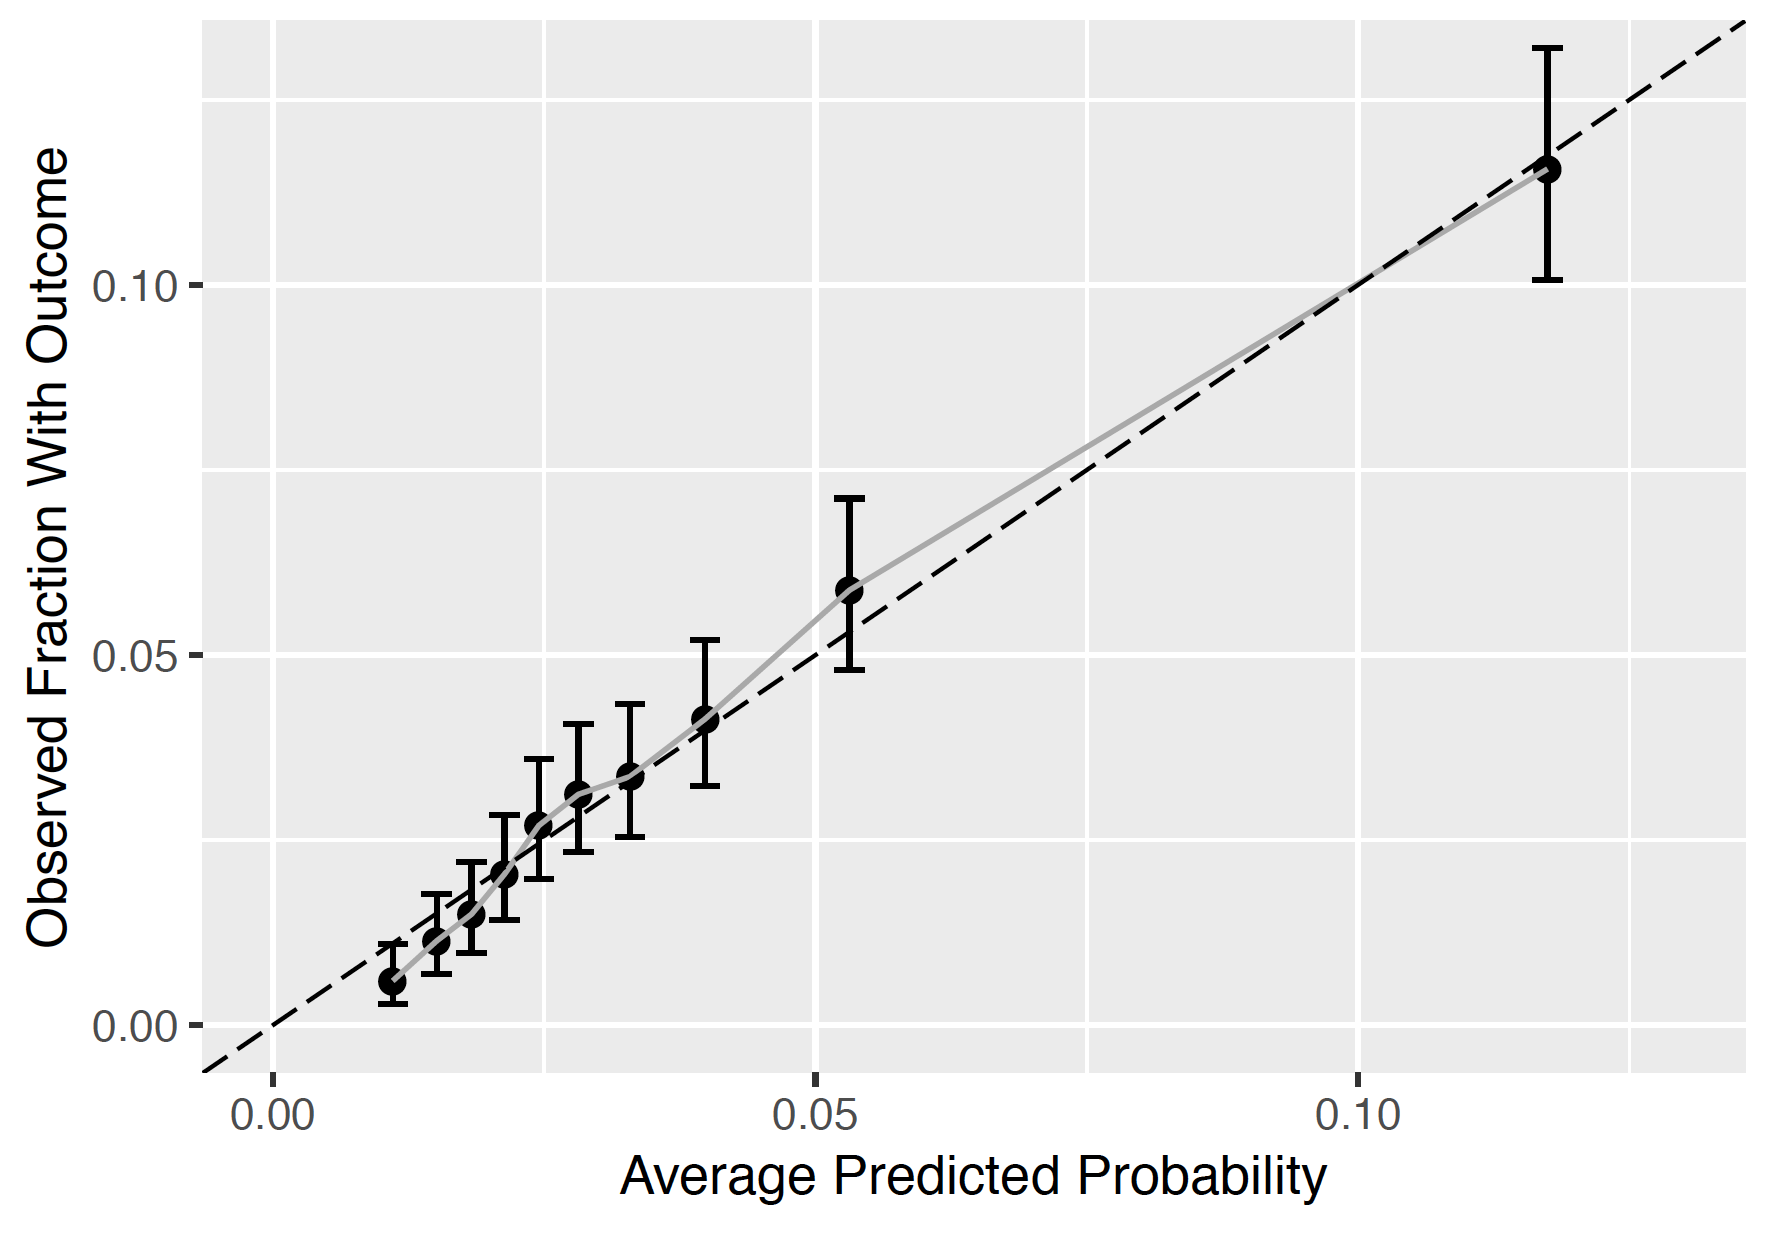
\includegraphics{sparseCalibration.png}

\newpage

\hypertarget{smooth-calibration}{%
\subsection{Smooth Calibration}\label{smooth-calibration}}

Similar to the traditional calibration shown above the Smooth
Calibration plot shows the relationship between predicted and observed
risk. the major difference is that the smooth fit allows for a more fine
grained examination of this. Whereas the traditional plot will be
heavily influenced by the areas with the highest density of data the
smooth plot will provide the same information for this region as well as
a more accurate interpretation of areas with lower density. the plot
also contains information on the distribution of the outcomes relative
to predicted risk.

However, the increased information gain comes at a computational cost.
It is recommended to use the traditional plot for examination and then
to produce the smooth plot for final versions. To create the smooth
calibarion plot you have to run the follow command:

\begin{Shaded}
\begin{Highlighting}[]
\KeywordTok{plotSmoothCalibration}\NormalTok{(lrResults)}
\end{Highlighting}
\end{Shaded}

See the help function for more information, on how to set the smoothing
method etc.

The example below is from another study that better demonstrates the
impact of using a smooth calibration plot. The default line fit would
not highlight the miss-calibration at the lower predicted probability
levels that well.

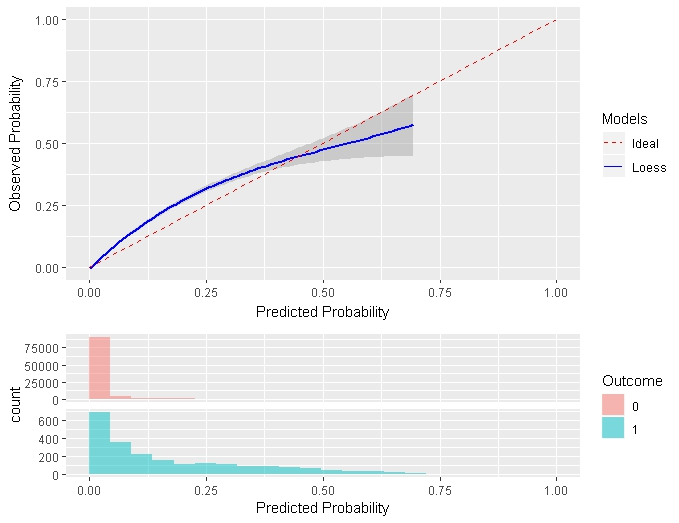
\includegraphics{smoothCalibration.jpeg}

\newpage \#\# Preference distribution

The preference distribution plots are the preference score distributions
corresponding to i) people in the test set with the outcome (red) and
ii) people in the test set without the outcome (blue).

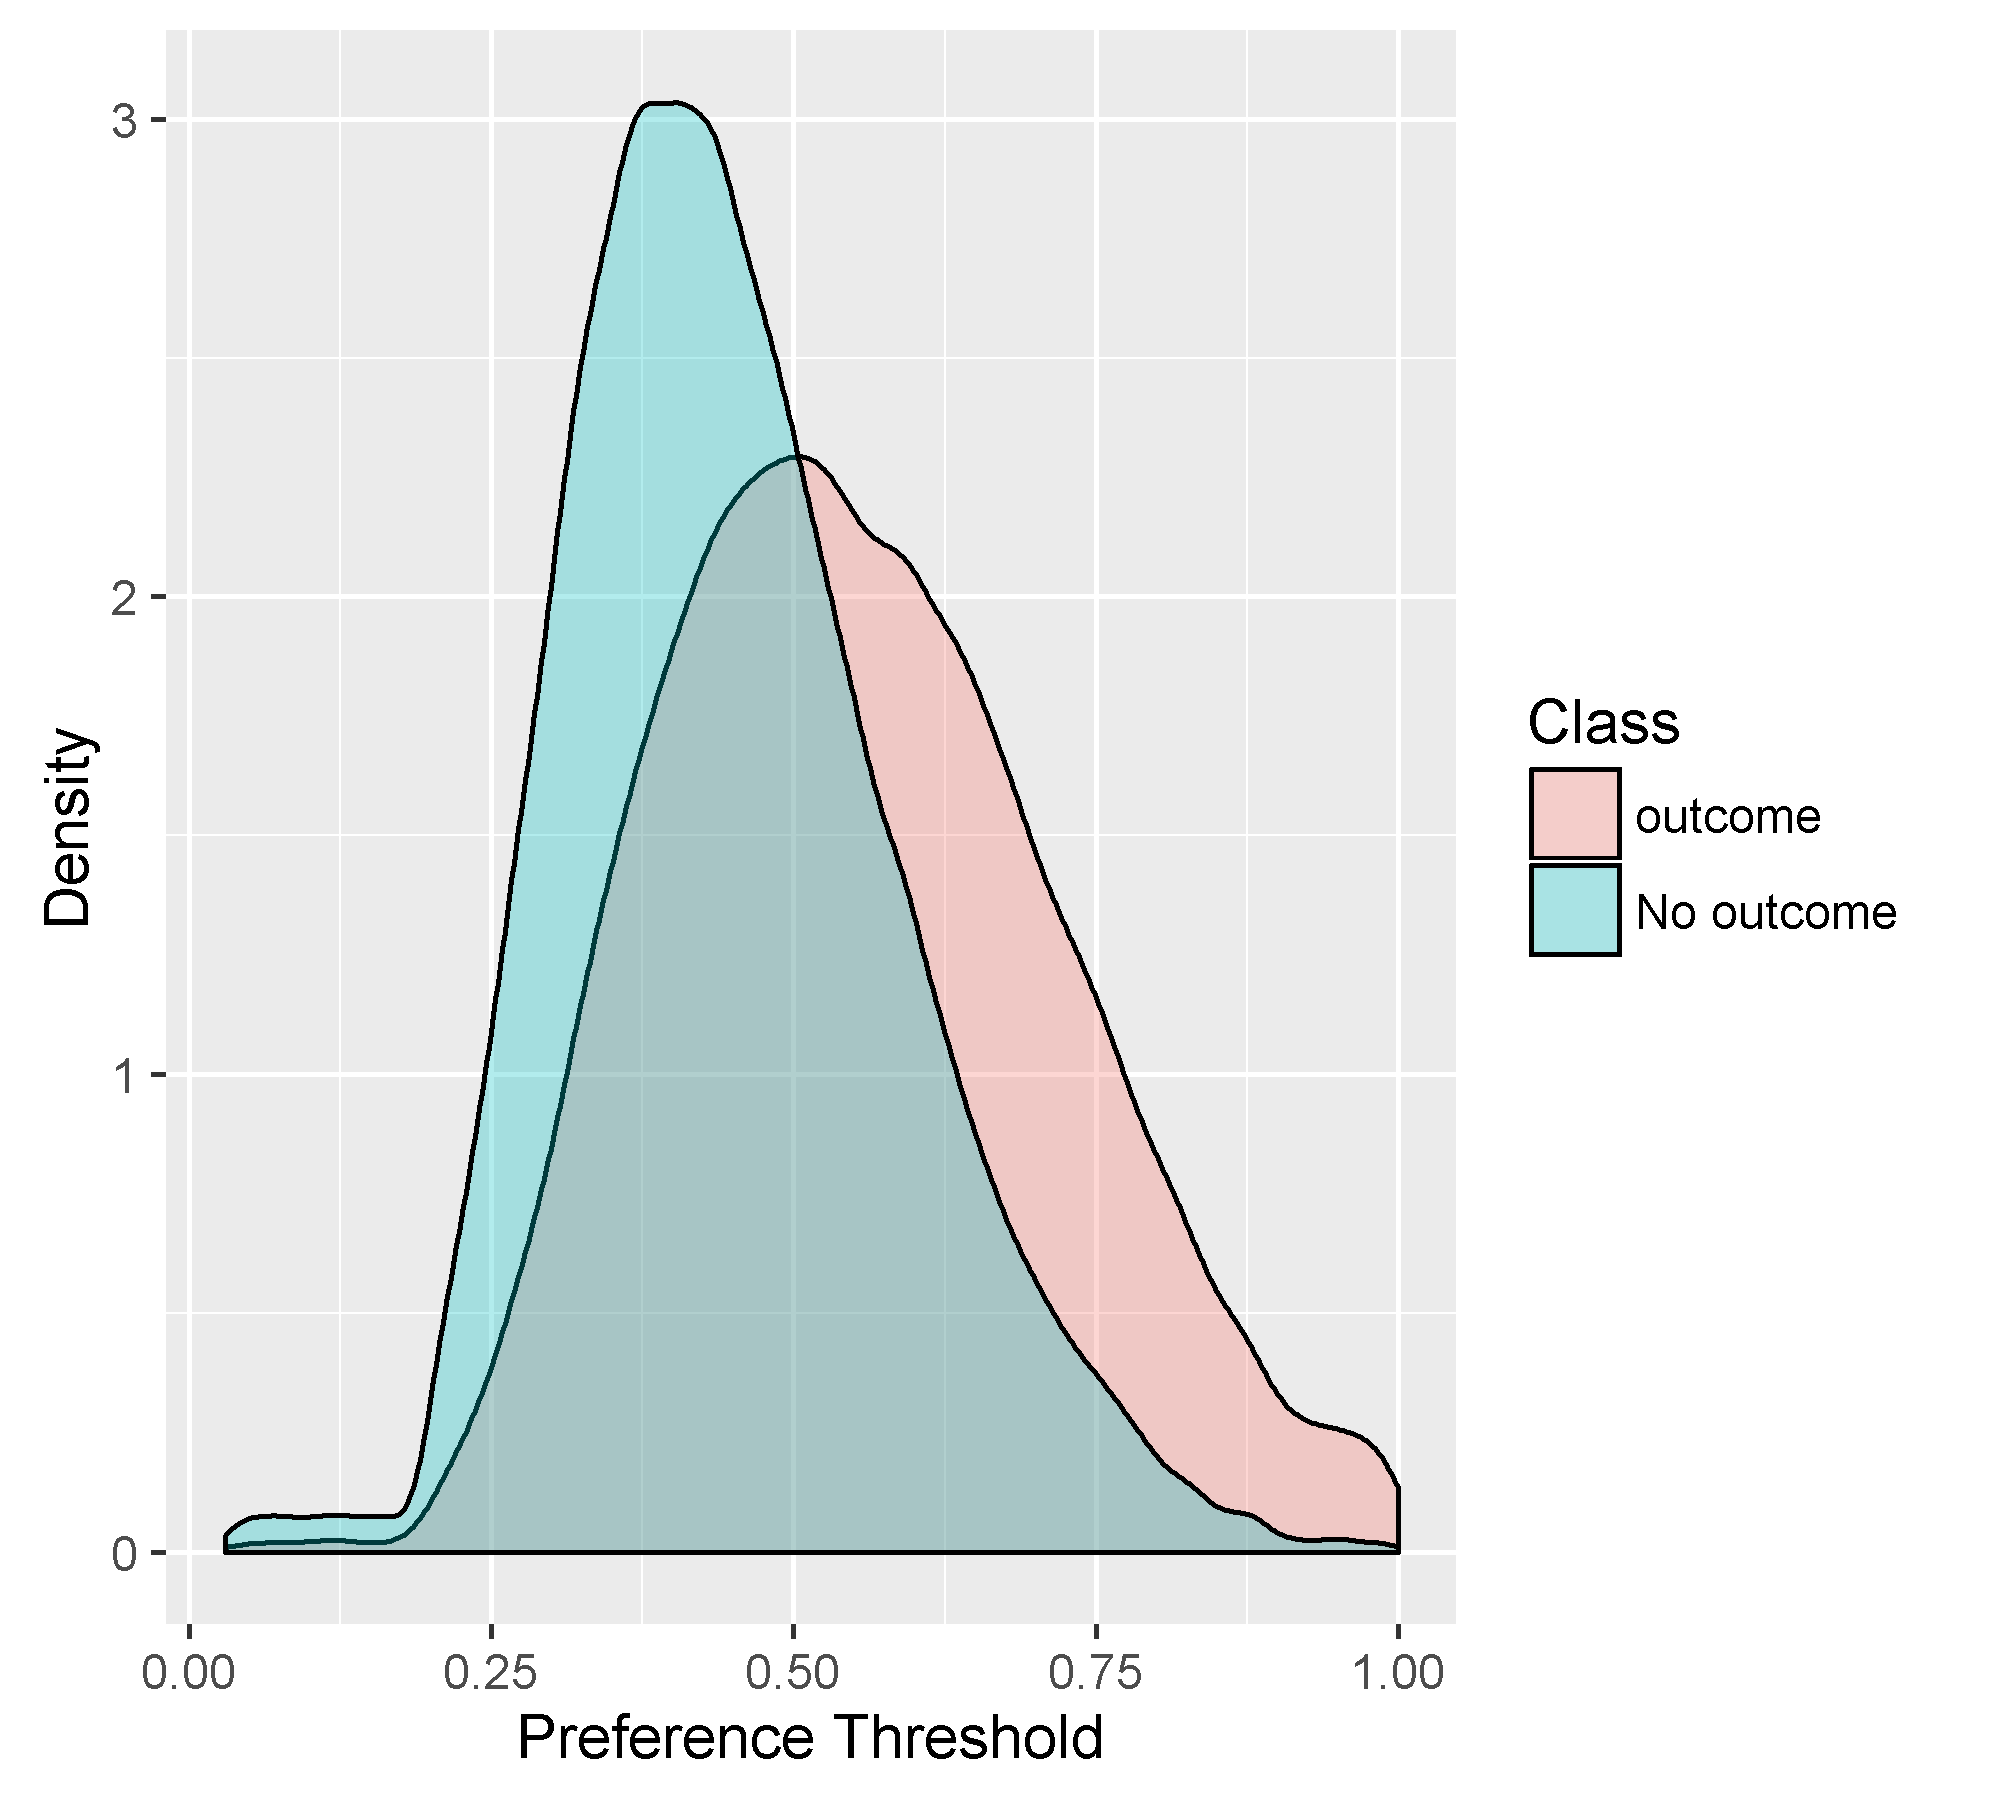
\includegraphics{preferencePDF.png}

\newpage \#\# Predicted probability distribution

The prediction distribution box plots are for the predicted risks of the
people in the test set with the outcome (class 1: blue) and without the
outcome (class 0: red).

The box plots in the Figure show that the predicted probability of the
outcome is indeed higher for those with the outcome but there is also
overlap between the two distribution which lead to an imperfect
discrimination.

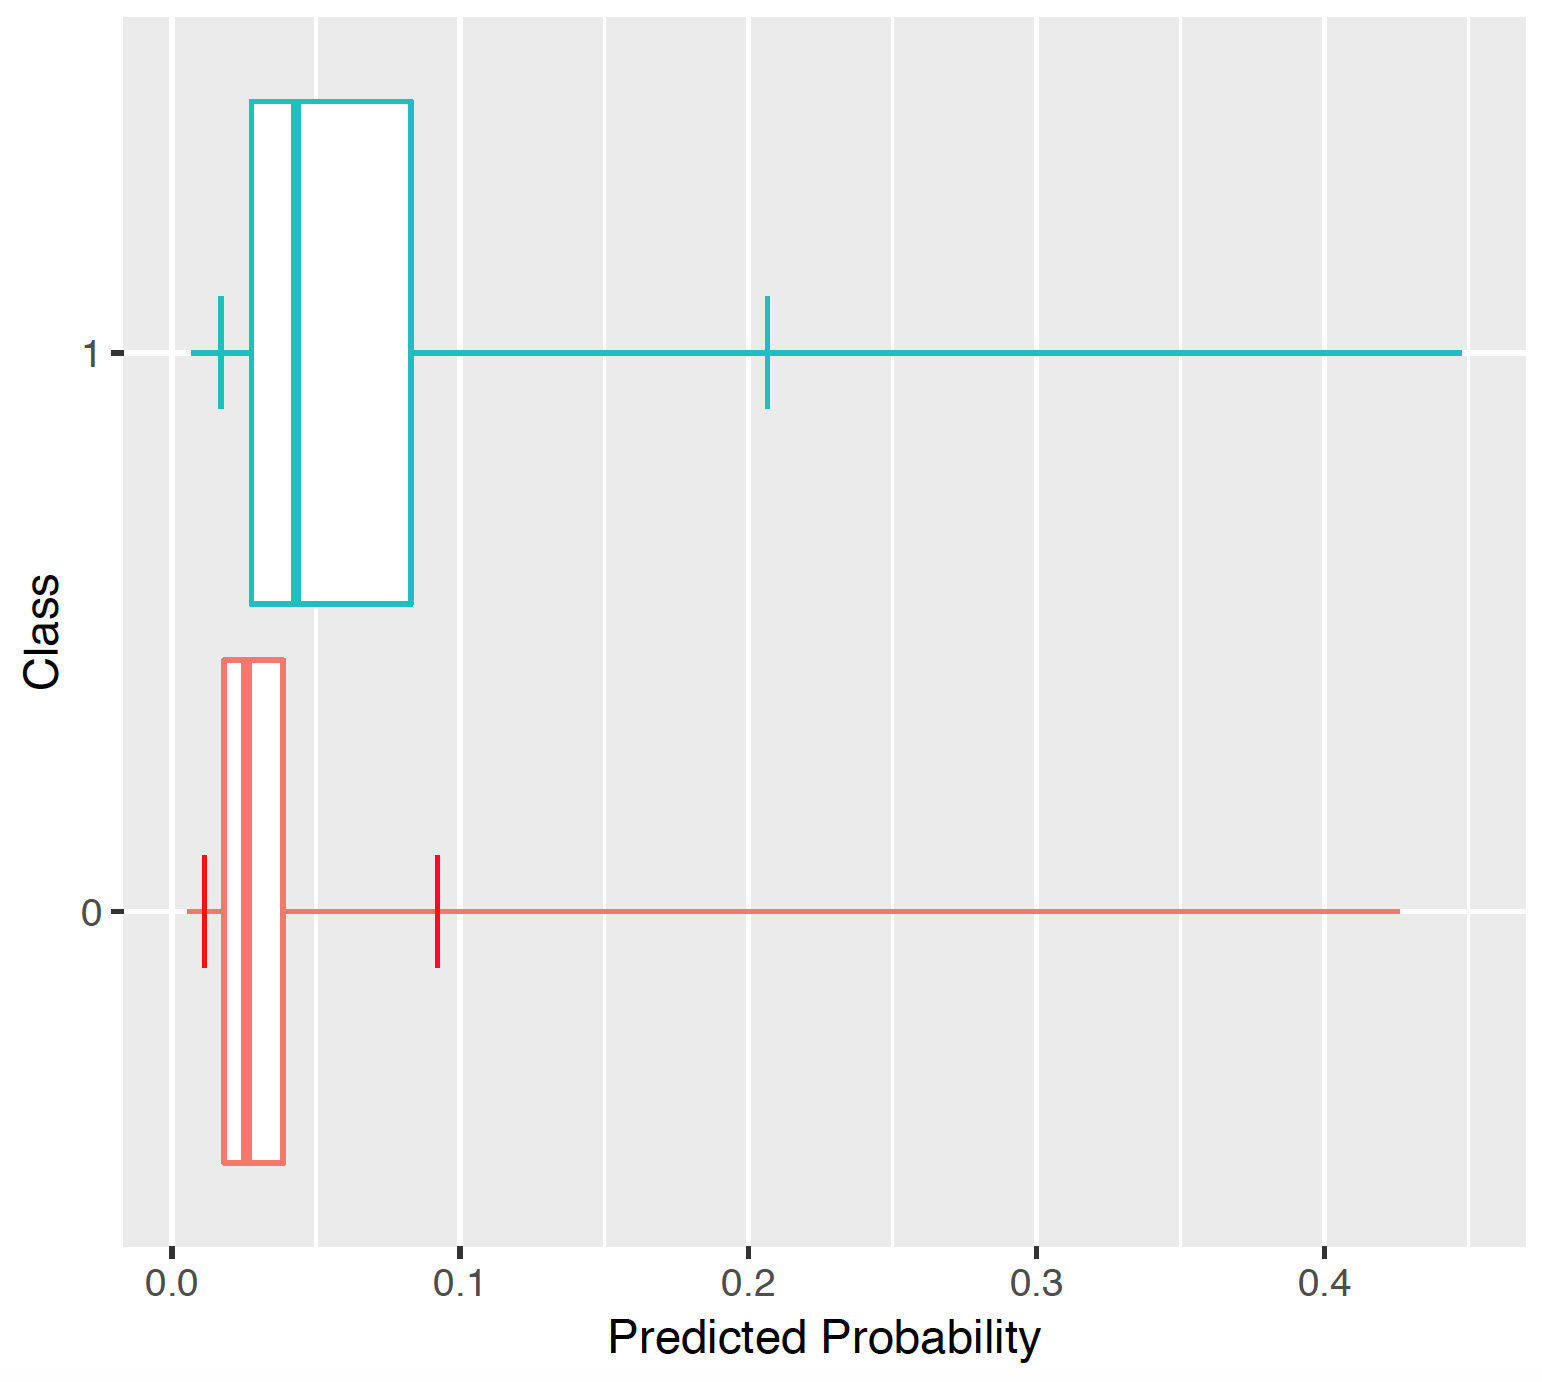
\includegraphics{predictionDistribution.png}

\newpage \#\# Test-Train similarity

The test-train similarity is assessed by plotting the mean covariate
values in the train set against those in the test set for people with
and without the outcome.

The results for our example of look very promising since the mean values
of the covariates are on the diagonal.

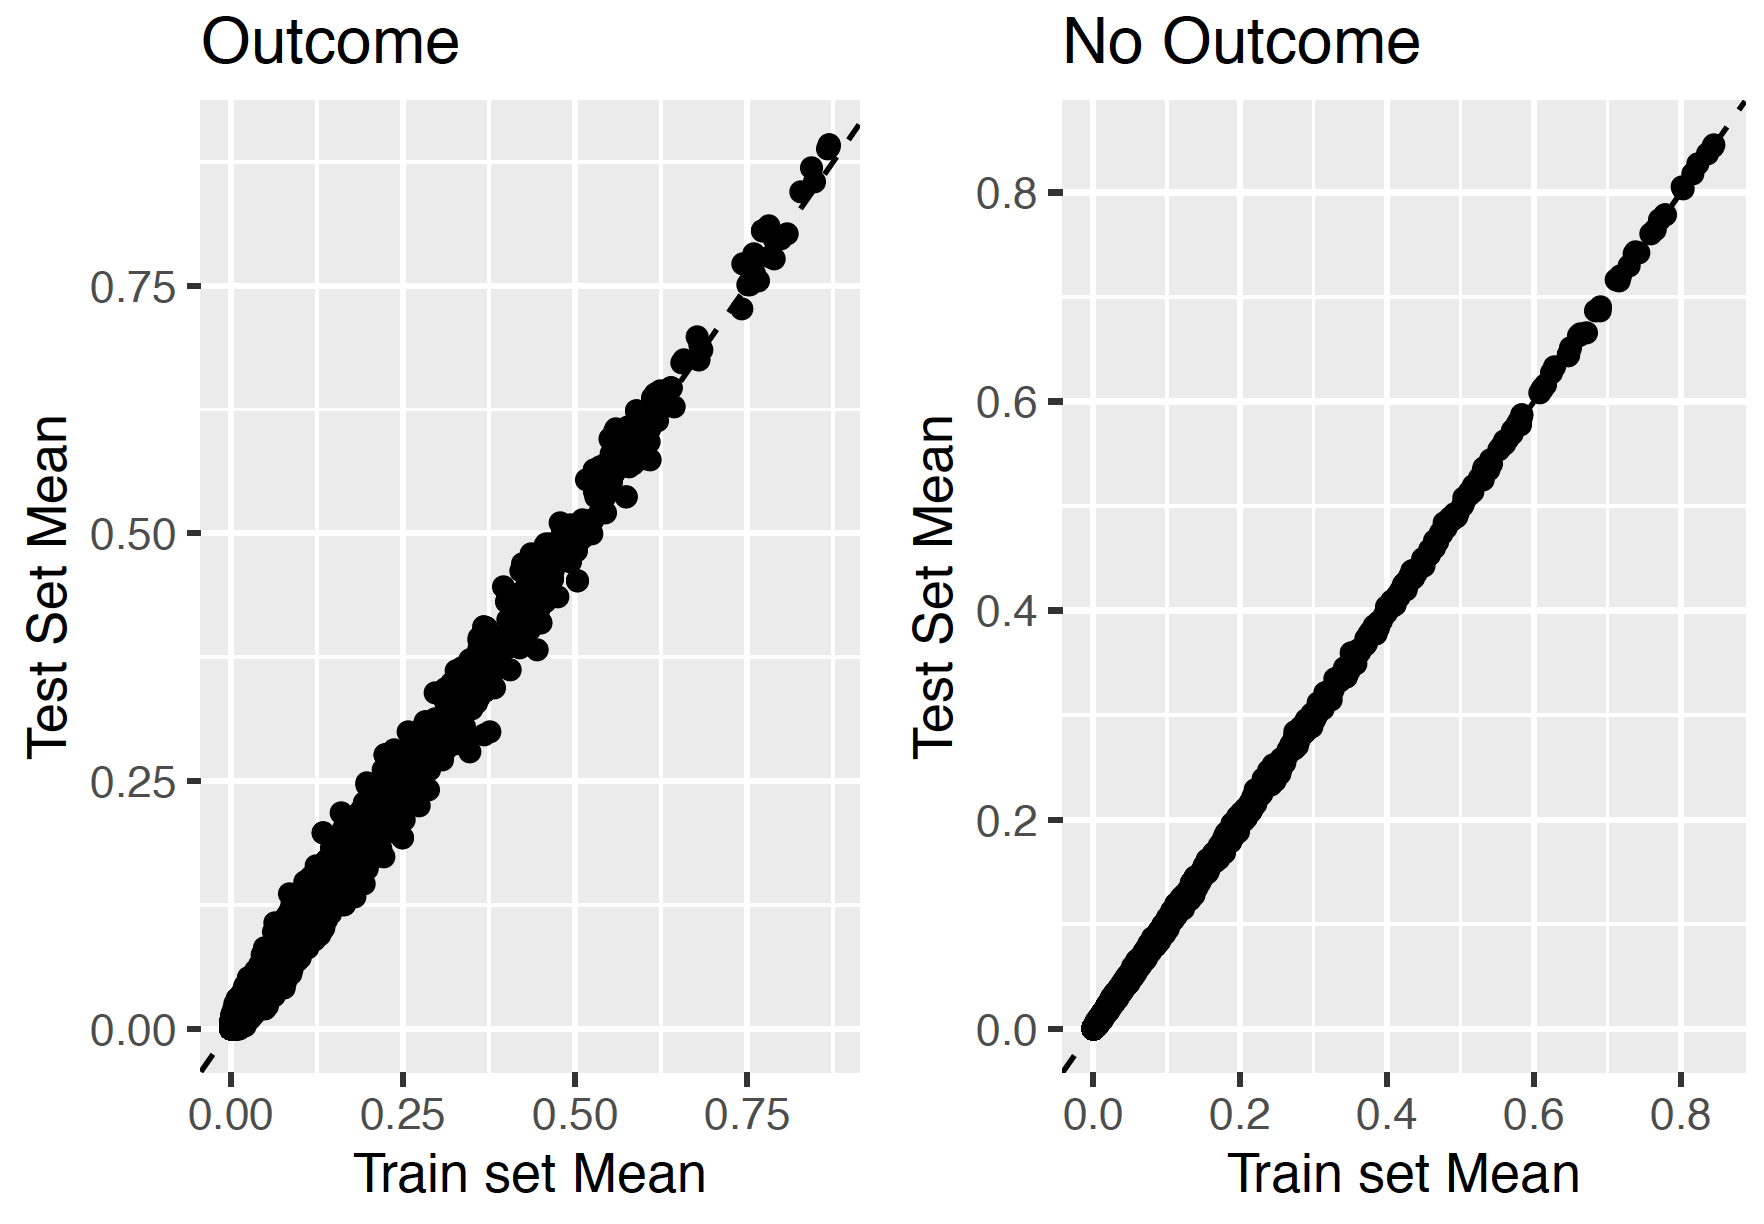
\includegraphics{generalizability.png}

\newpage \#\# Variable scatter plot

The variable scatter plot shows the mean covariate value for the people
with the outcome against the mean covariate value for the people without
the outcome. The color of the dots corresponds to the inclusion (green)
or exclusion in the model (blue), respectively. It is highly recommended
to use the Shiny App since this allows you to hoover over a covariate to
show more details (name, value etc).

The plot shows that the mean of most of the covariates is higher for
subjects with the outcome compared to those without.

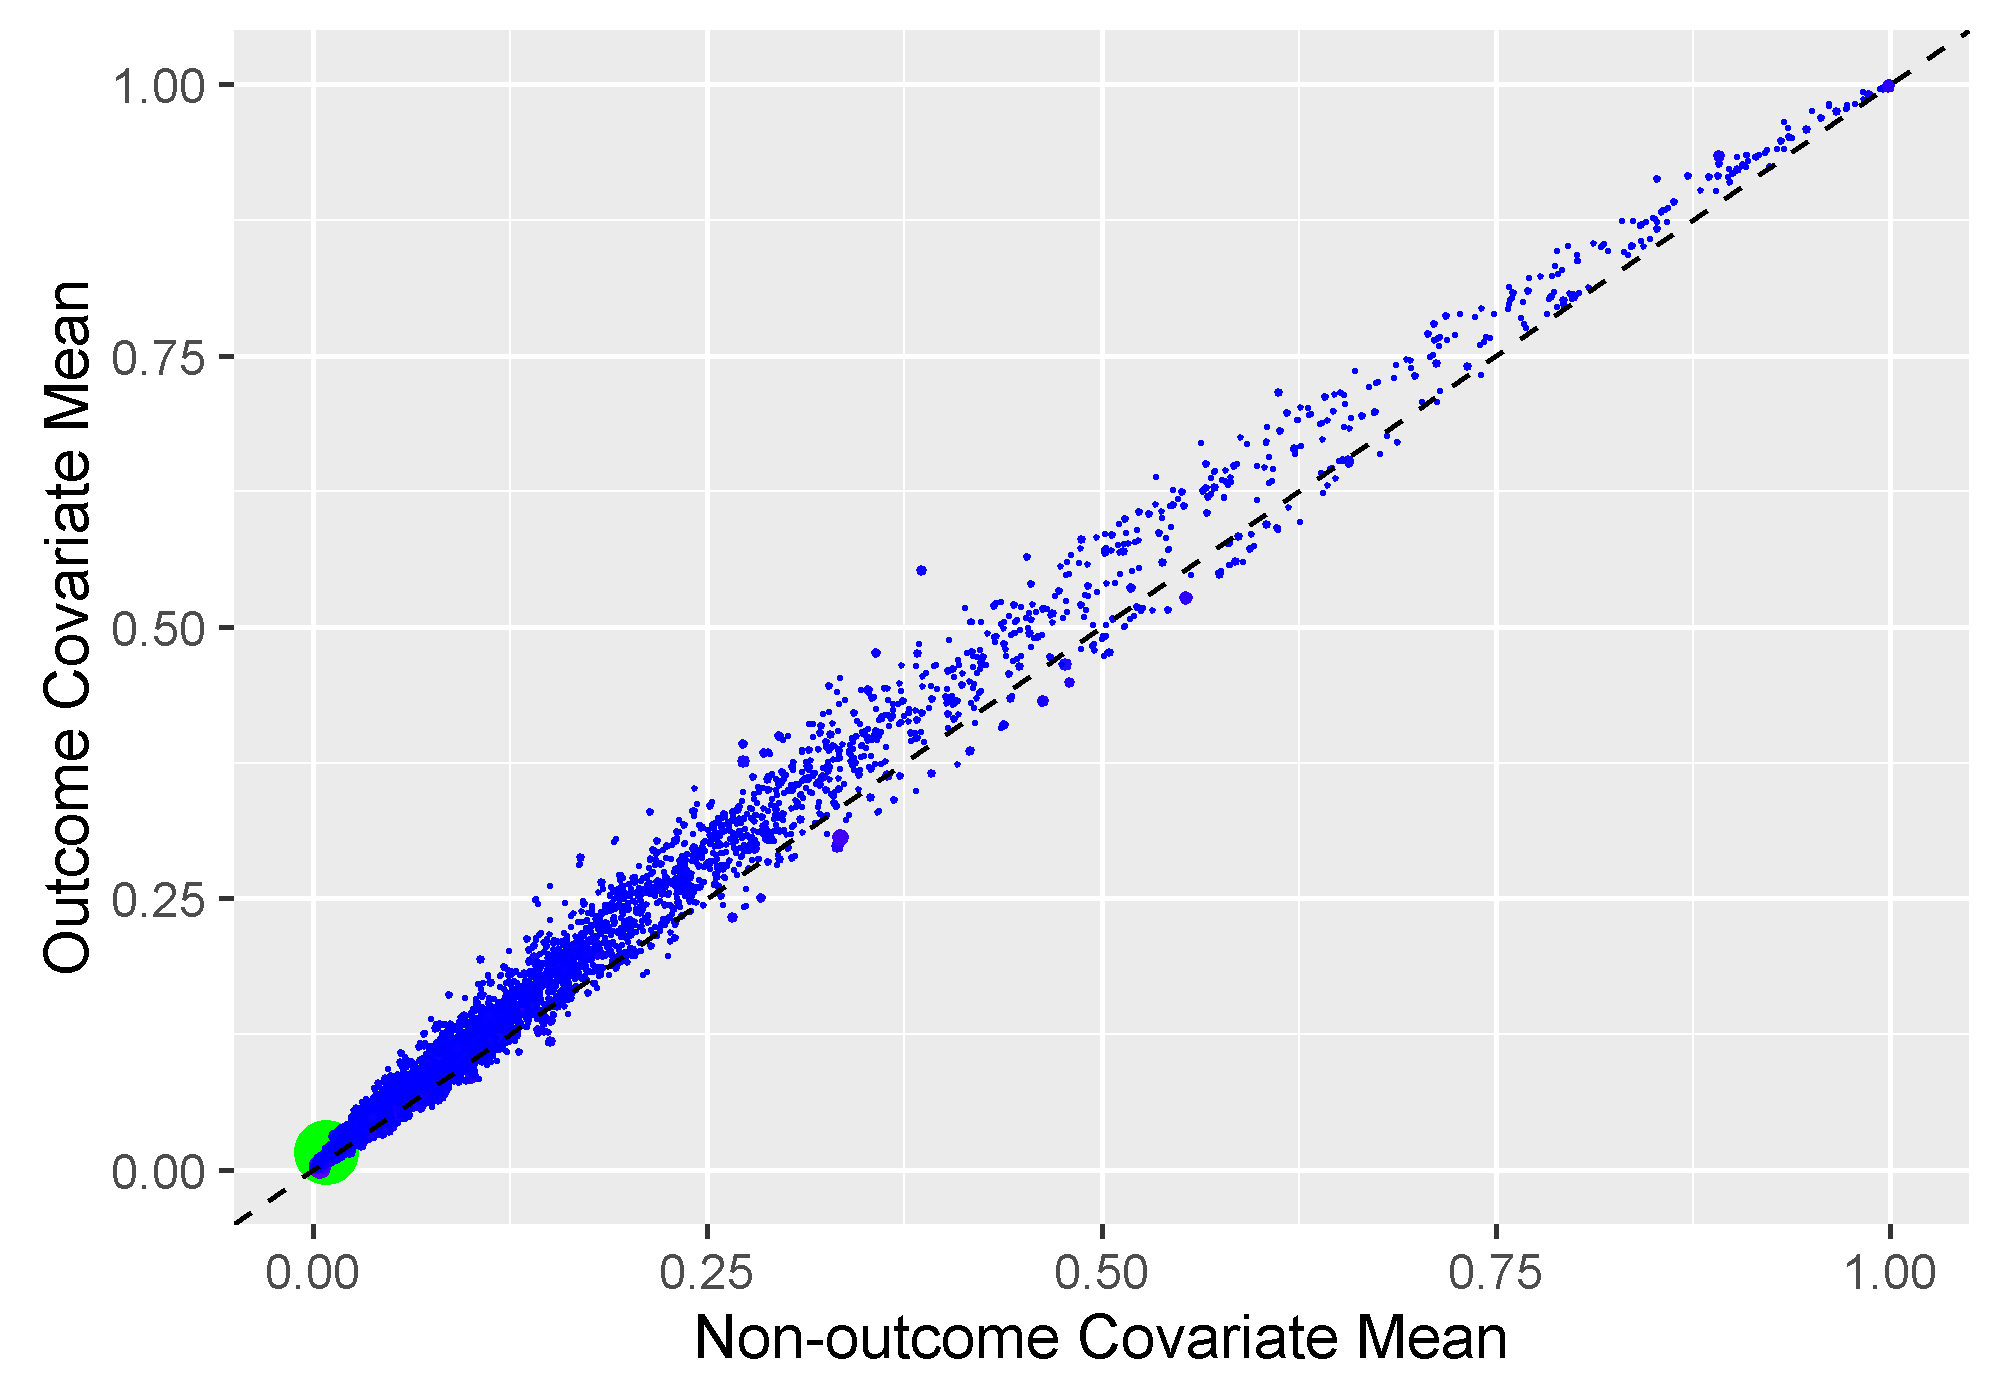
\includegraphics{variableScatterplot.png}

\newpage \#\# Precision recall

Precision (P) is defined as the number of true positives (Tp) over the
number of true positives plus the number of false positives (Fp).

\begin{Shaded}
\begin{Highlighting}[]
\NormalTok{P <-}\StringTok{ }\NormalTok{Tp}\OperatorTok{/}\NormalTok{(Tp }\OperatorTok{+}\StringTok{ }\NormalTok{Fp)}
\end{Highlighting}
\end{Shaded}

Recall (R) is defined as the number of true positives (Tp) over the
number of true positives plus the number of false negatives (Fn).

\begin{Shaded}
\begin{Highlighting}[]
\NormalTok{R <-}\StringTok{ }\NormalTok{Tp}\OperatorTok{/}\NormalTok{(Tp }\OperatorTok{+}\StringTok{ }\NormalTok{Fn)}
\end{Highlighting}
\end{Shaded}

These quantities are also related to the (F1) score, which is defined as
the harmonic mean of precision and recall.

\begin{Shaded}
\begin{Highlighting}[]
\NormalTok{F1 <-}\StringTok{ }\DecValTok{2} \OperatorTok{*}\StringTok{ }\NormalTok{P }\OperatorTok{*}\StringTok{ }\NormalTok{R}\OperatorTok{/}\NormalTok{(P }\OperatorTok{+}\StringTok{ }\NormalTok{R)}
\end{Highlighting}
\end{Shaded}

Note that the precision can either decrease or increase if the threshold
is lowered. Lowering the threshold of a classifier may increase the
denominator, by increasing the number of results returned. If the
threshold was previously set too high, the new results may all be true
positives, which will increase precision. If the previous threshold was
about right or too low, further lowering the threshold will introduce
false positives, decreasing precision.

For Recall the denominator does not depend on the classifier threshold
(Tp+Fn is a constant). This means that lowering the classifier threshold
may increase recall, by increasing the number of true positive results.
It is also possible that lowering the threshold may leave recall
unchanged, while the precision fluctuates.

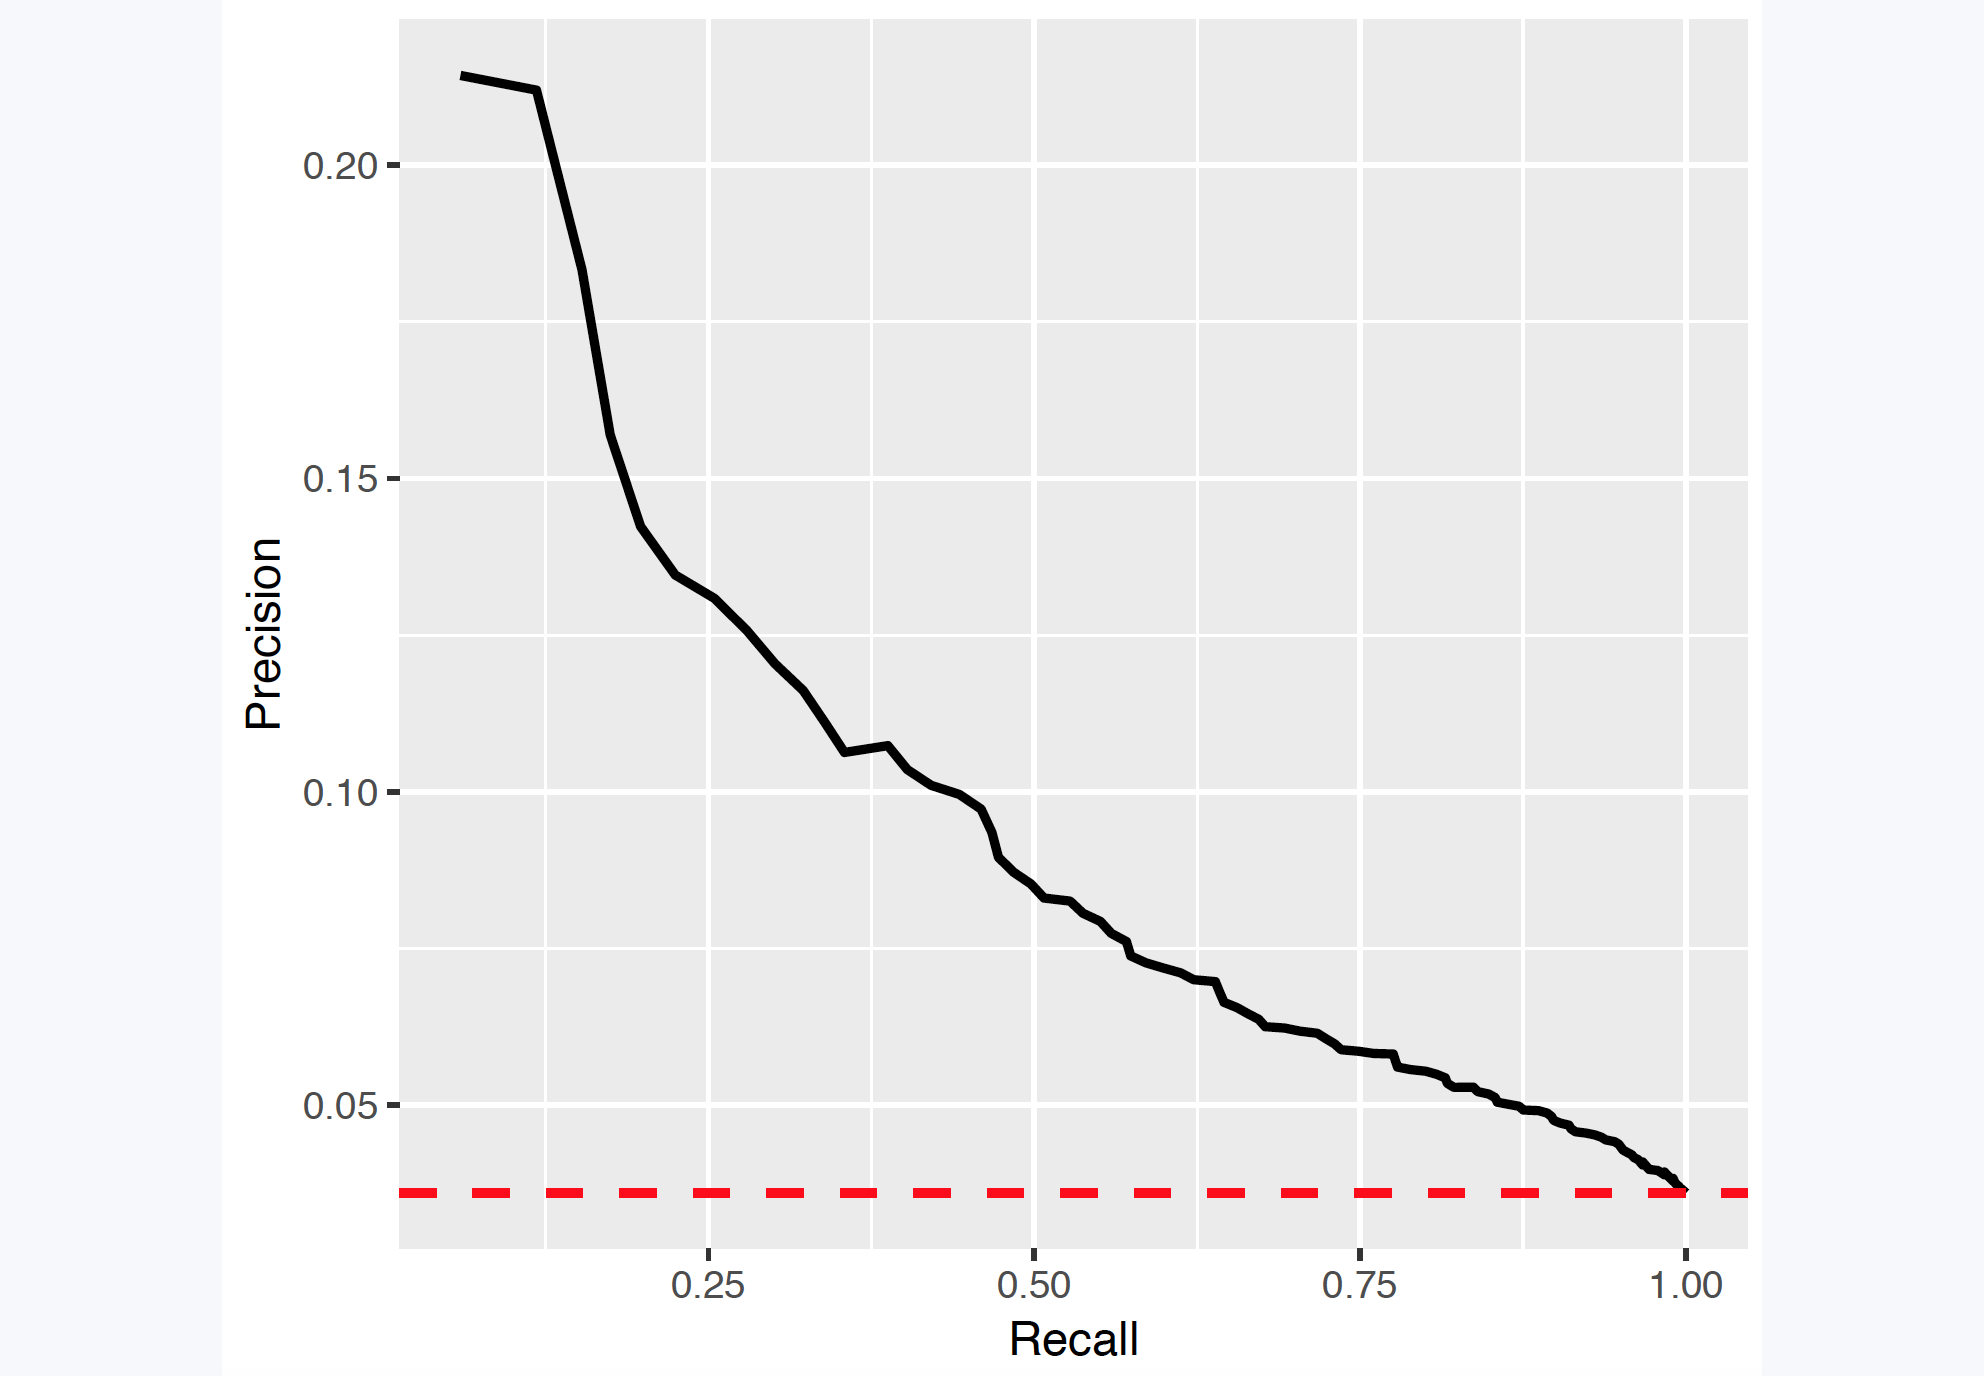
\includegraphics{precisionRecall.png}

\newpage \#\# Demographic summary

This plot shows for females and males the expected and observed risk in
different age groups together with a confidence area.

The results show that our model is well calibrated across gender and age
groups.

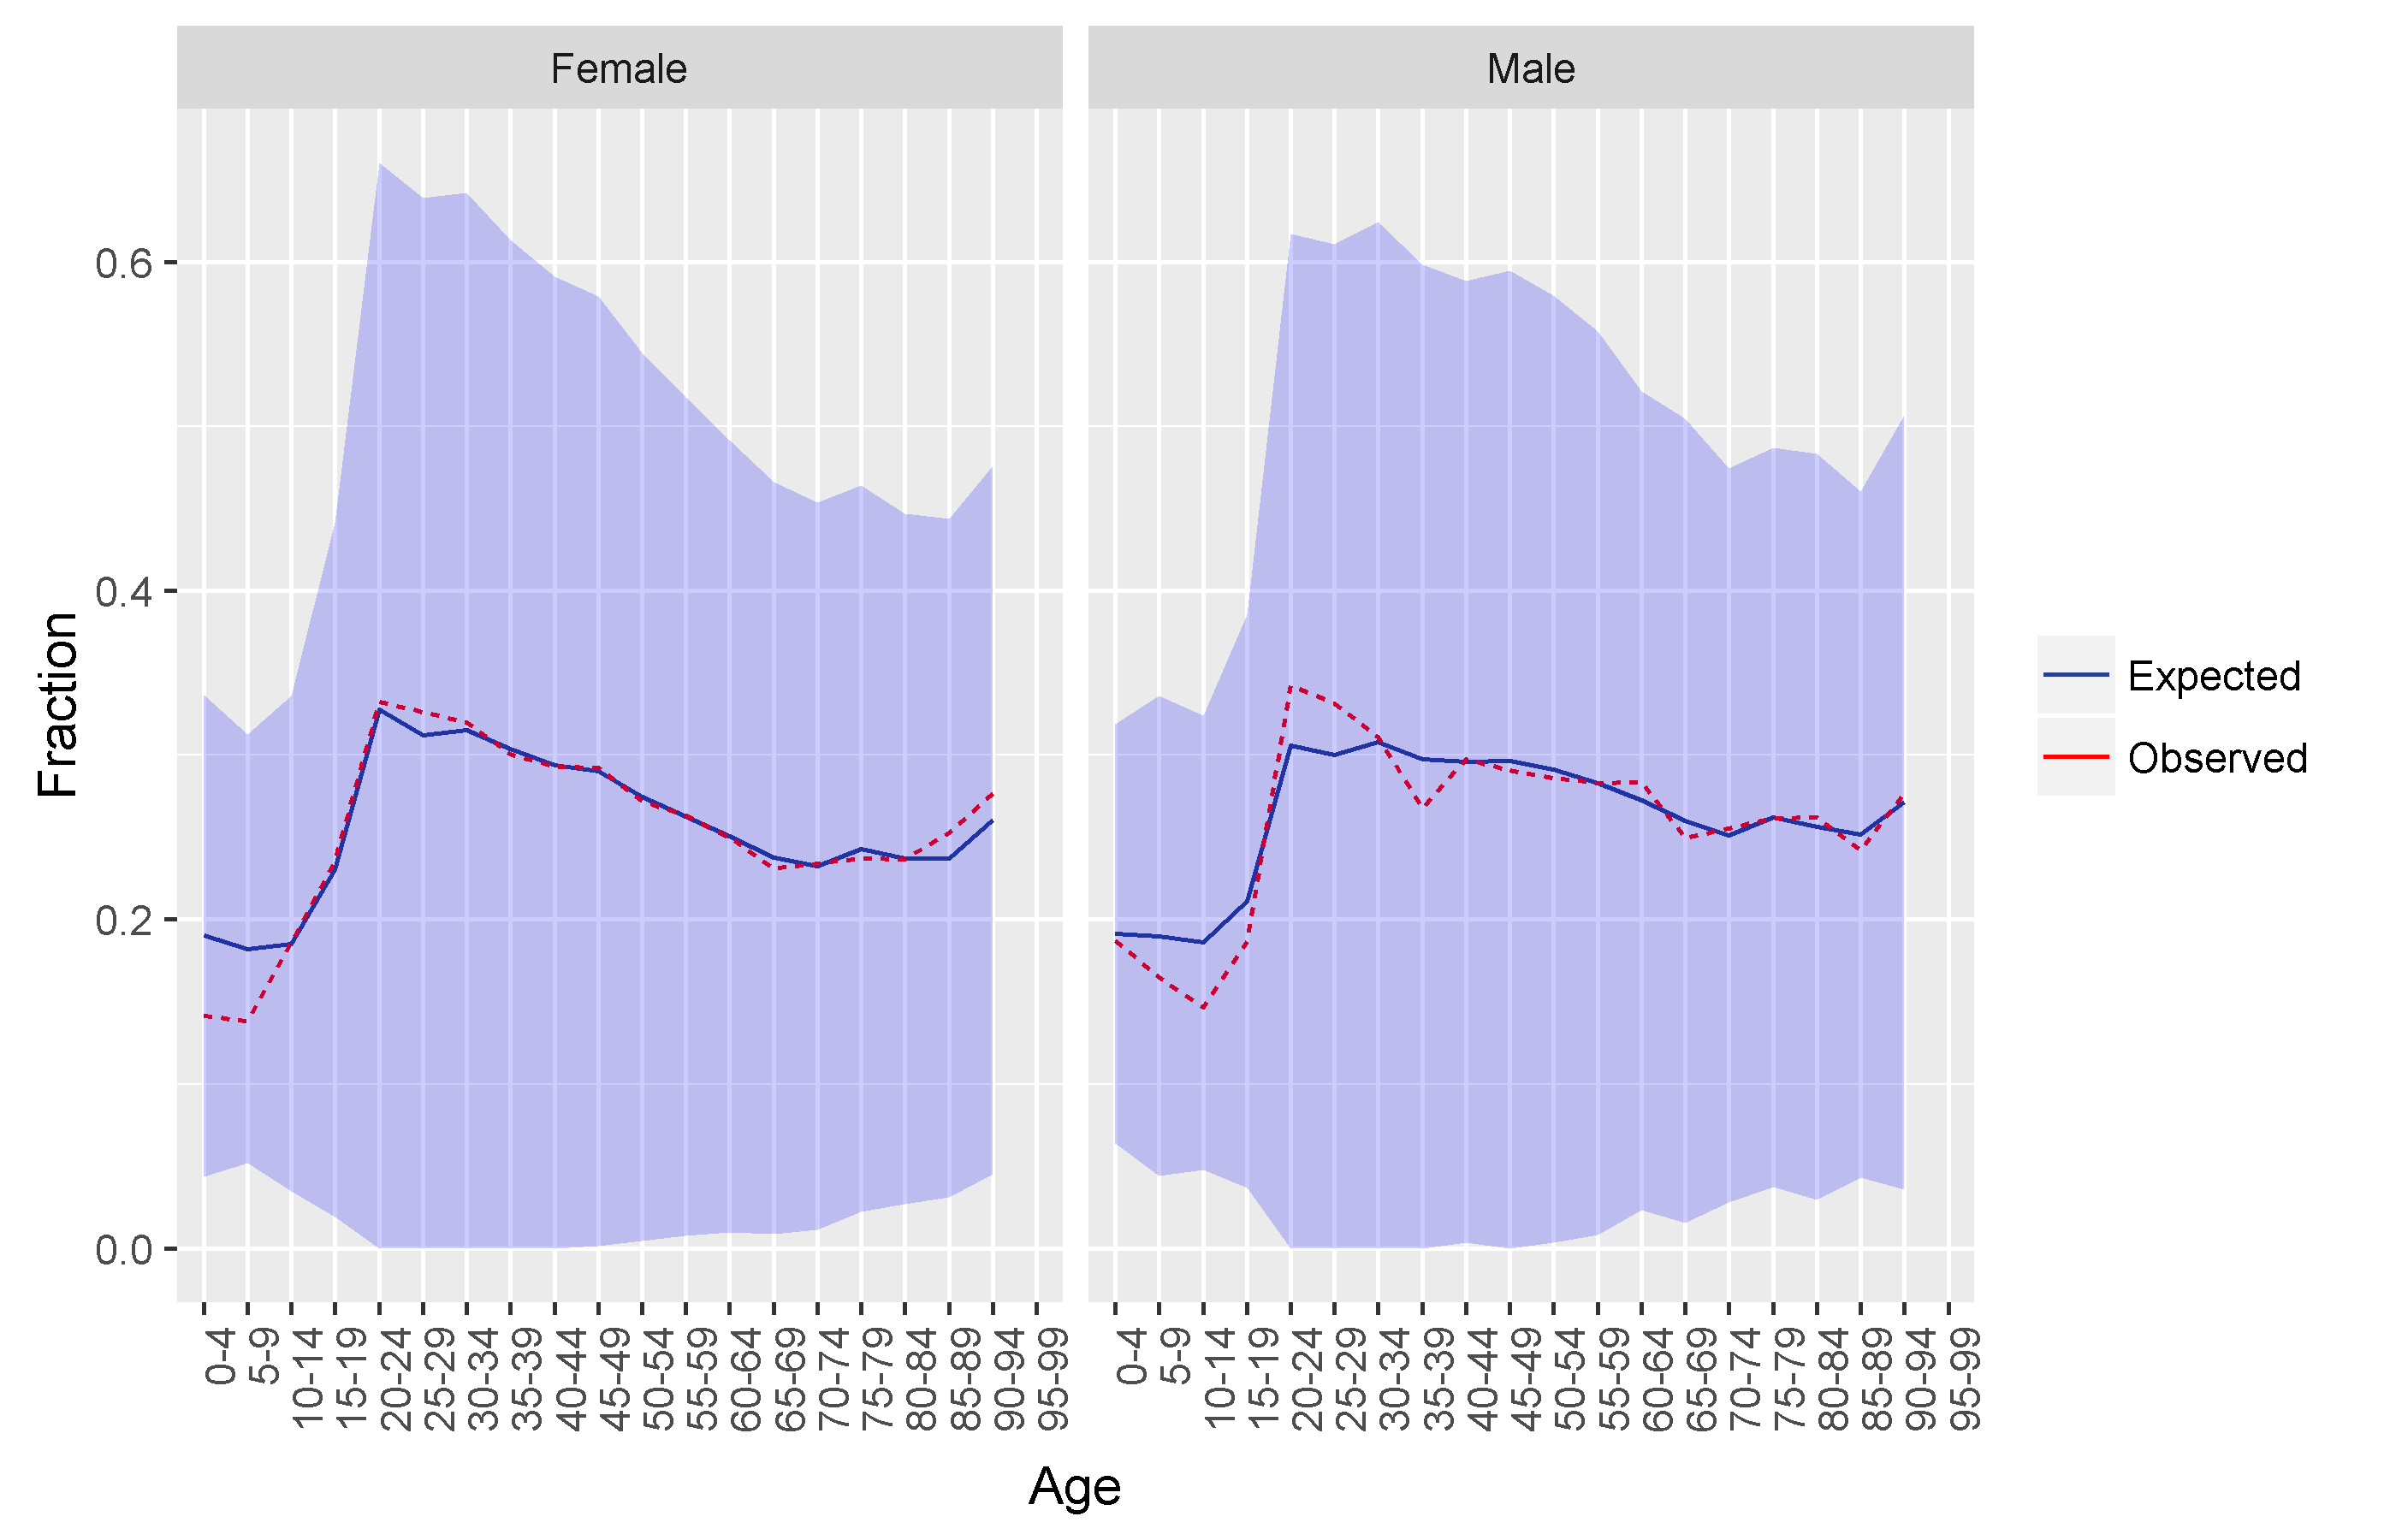
\includegraphics{demographicSummary.png}

\newpage \# External validation

We recommend to always perform external validation, i.e.~apply the final
model on as much new datasets as feasible and evaluate its performance.

\begin{Shaded}
\begin{Highlighting}[]
\CommentTok{# load the trained model}
\NormalTok{plpModel <-}\StringTok{ }\KeywordTok{loadPlpModel}\NormalTok{(}\KeywordTok{getwd}\NormalTok{(),}\StringTok{'model'}\NormalTok{)}

\CommentTok{#load the new plpData and create the population}
\NormalTok{plpData <-}\StringTok{ }\KeywordTok{loadPlpData}\NormalTok{(}\KeywordTok{getwd}\NormalTok{(),}\StringTok{'data'}\NormalTok{)}
\NormalTok{population <-}\StringTok{ }\KeywordTok{createStudyPopulation}\NormalTok{(plpData, }
                                    \DataTypeTok{outcomeId =} \DecValTok{2}\NormalTok{, }
                                    \DataTypeTok{includeAllOutcomes =} \OtherTok{TRUE}\NormalTok{, }
                                    \DataTypeTok{firstExposureOnly =} \OtherTok{TRUE}\NormalTok{, }
                                    \DataTypeTok{washoutPeriod =} \DecValTok{365}\NormalTok{, }
                                    \DataTypeTok{removeSubjectsWithPriorOutcome =} \OtherTok{TRUE}\NormalTok{, }
                                    \DataTypeTok{priorOutcomeLookback =} \DecValTok{365}\NormalTok{,}
                                    \DataTypeTok{riskWindowStart =} \DecValTok{1}\NormalTok{,}
                                    \DataTypeTok{requireTimeAtRisk =} \OtherTok{FALSE}\NormalTok{,}
                                    \DataTypeTok{riskWindowEnd =} \DecValTok{365}
\NormalTok{)}

\CommentTok{# apply the trained model on the new data}
\NormalTok{validationResults <-}\StringTok{ }\KeywordTok{applyModel}\NormalTok{(population,plpData,plpModel)}
\end{Highlighting}
\end{Shaded}

To make things easier we also provide a function for performing external
validation of a model across one or multiple datasets:

\begin{Shaded}
\begin{Highlighting}[]
\CommentTok{# load the trained model}
\NormalTok{plpResult <-}\StringTok{ }\KeywordTok{loadPlpResult}\NormalTok{(}\KeywordTok{getwd}\NormalTok{(),}\StringTok{'plpResult'}\NormalTok{)}

\NormalTok{connectionDetails <-}\StringTok{ }\KeywordTok{createConnectionDetails}\NormalTok{(}\DataTypeTok{dbms =} \StringTok{"postgresql"}\NormalTok{, }
                                             \DataTypeTok{server =} \StringTok{"localhost/ohdsi"}\NormalTok{, }
                                             \DataTypeTok{user =} \StringTok{"joe"}\NormalTok{, }
                                             \DataTypeTok{password =} \StringTok{"supersecret"}\NormalTok{)}

\NormalTok{validation <-}\StringTok{ }\KeywordTok{externalValidatePlp}\NormalTok{(}\DataTypeTok{plpResult =}\NormalTok{ plpResult, }
                                  \DataTypeTok{connectionDetails =}\NormalTok{ connectionDetails,}
                                  \DataTypeTok{validationSchemaTarget =} \StringTok{'new_cohort_schema'}\NormalTok{,}
                                  \DataTypeTok{validationSchemaOutcome =} \StringTok{'new_cohort_schema'}\NormalTok{,}
                                  \DataTypeTok{validationSchemaCdm =} \StringTok{'new_cdm_schema'}\NormalTok{, }
                                  \DataTypeTok{validationTableTarget =} \StringTok{'cohort_table'}\NormalTok{,}
                                  \DataTypeTok{validationTableOutcome =} \StringTok{'cohort_table'}\NormalTok{, }
                                  \DataTypeTok{validationIdTarget =} \StringTok{'cohort_id'}\NormalTok{, }
                                  \DataTypeTok{validationIdOutcome =} \StringTok{'outcome_id'}\NormalTok{, }
                                  \DataTypeTok{keepPrediction =}\NormalTok{ T}
\NormalTok{)}
\end{Highlighting}
\end{Shaded}

This will extract the new plpData from the specified schemas and cohort
tables. It will then apply the same population settings and the trained
plp model. Finally, it will evaluate the performance and return the
standard output as \texttt{validation\$performance} and if
keepPrediction is TRUE then it will also return the prediction on the
population as \texttt{validation\$prediction}. They can be inserted into
the shiny app for viewing the model and validation by running:
\texttt{viewPlp(runPlp=plpResult,\ validatePlp=validation\ )}.

If you want to validate on multiple databases available you can insert
the new schemas and cohort tables as a list:

\begin{Shaded}
\begin{Highlighting}[]
\CommentTok{# load the trained model}
\NormalTok{plpResult <-}\StringTok{ }\KeywordTok{loadPlpResult}\NormalTok{(}\KeywordTok{getwd}\NormalTok{(),}\StringTok{'plpResult'}\NormalTok{)}

\NormalTok{connectionDetails <-}\StringTok{ }\KeywordTok{createConnectionDetails}\NormalTok{(}\DataTypeTok{dbms =} \StringTok{"postgresql"}\NormalTok{, }
                                             \DataTypeTok{server =} \StringTok{"localhost/ohdsi"}\NormalTok{, }
                                             \DataTypeTok{user =} \StringTok{"joe"}\NormalTok{, }
                                             \DataTypeTok{password =} \StringTok{"supersecret"}\NormalTok{)}

\NormalTok{validation <-}\StringTok{ }\KeywordTok{externalValidatePlp}\NormalTok{(}\DataTypeTok{plpResult =}\NormalTok{ plpResult, }
                                  \DataTypeTok{connectionDetails =}\NormalTok{ connectionDetails,}
                                  \DataTypeTok{validationSchemaTarget =} \KeywordTok{list}\NormalTok{(}\StringTok{'new_cohort_schema1'}\NormalTok{,}
                                                                \StringTok{'new_cohort_schema2'}\NormalTok{),}
                                  \DataTypeTok{validationSchemaOutcome =} \KeywordTok{list}\NormalTok{(}\StringTok{'new_cohort_schema1'}\NormalTok{,}
                                                                 \StringTok{'new_cohort_schema2'}\NormalTok{),}
                                  \DataTypeTok{validationSchemaCdm =} \KeywordTok{list}\NormalTok{(}\StringTok{'new_cdm_schema1'}\NormalTok{,}
                                                             \StringTok{'new_cdm_schema2'}\NormalTok{), }
                                  \DataTypeTok{validationTableTarget =} \KeywordTok{list}\NormalTok{(}\StringTok{'new_cohort_table1'}\NormalTok{,}
                                                               \StringTok{'new_cohort_table2'}\NormalTok{),}
                                  \DataTypeTok{validationTableOutcome =} \KeywordTok{list}\NormalTok{(}\StringTok{'new_cohort_table1'}\NormalTok{,}
                                                                \StringTok{'new_cohort_table2'}\NormalTok{),}
                                  \DataTypeTok{validationIdTarget =} \StringTok{'cohort_id'}\NormalTok{, }
                                  \DataTypeTok{validationIdOutcome =} \StringTok{'outcome_id'}\NormalTok{, }
                                  \DataTypeTok{keepPrediction =}\NormalTok{ T}
\NormalTok{)}
\end{Highlighting}
\end{Shaded}

\hypertarget{journal-paper-generation}{%
\section{Journal paper generation}\label{journal-paper-generation}}

We have added functionality to automatically generate a word document
you can use as start of a journal paper. It contains many of the
generated study details and results. If you have performed external
validation these results will can be added as well. Optionally, you can
add a ``Table 1'' that contains data on many covariates for the target
population.

You can create the draft journal paper by running this function:

\begin{Shaded}
\begin{Highlighting}[]
\KeywordTok{createPlpJournalDocument}\NormalTok{(}\DataTypeTok{plpResult =} \OperatorTok{<}\NormalTok{your plp results}\OperatorTok{>}\NormalTok{, }
                         \DataTypeTok{plpValidation =} \OperatorTok{<}\NormalTok{your validation results}\OperatorTok{>}\NormalTok{,}
                         \DataTypeTok{plpData =} \OperatorTok{<}\NormalTok{your plp data}\OperatorTok{>}\NormalTok{, }
                         \DataTypeTok{targetName =} \StringTok{"<target population>"}\NormalTok{,}
                         \DataTypeTok{outcomeName =} \StringTok{"<outcome>"}\NormalTok{, }
                         \DataTypeTok{table1 =}\NormalTok{ F, }
                         \DataTypeTok{connectionDetails =} \OtherTok{NULL}\NormalTok{,}
                         \DataTypeTok{includeTrain =} \OtherTok{FALSE}\NormalTok{,}
                         \DataTypeTok{includeTest =} \OtherTok{TRUE}\NormalTok{,}
                         \DataTypeTok{includePredictionPicture =} \OtherTok{TRUE}\NormalTok{,}
                         \DataTypeTok{includeAttritionPlot =} \OtherTok{TRUE}\NormalTok{,}
                         \DataTypeTok{outputLocation =} \StringTok{"<your location>"}\NormalTok{)}\ErrorTok{)}
\end{Highlighting}
\end{Shaded}

For more details see the help page of the function.

\newpage

\hypertarget{other-functionality}{%
\section{Other functionality}\label{other-functionality}}

The package has much more functionality than described in this vignette
and contributions have been made my many persons in the OHDSI community.
The table below provides an overview:

\begin{longtable}[]{@{}lll@{}}
\toprule
\begin{minipage}[b]{0.18\columnwidth}\raggedright
Functionality\strut
\end{minipage} & \begin{minipage}[b]{0.55\columnwidth}\raggedright
Description\strut
\end{minipage} & \begin{minipage}[b]{0.18\columnwidth}\raggedright
Vignette\strut
\end{minipage}\tabularnewline
\midrule
\endhead
\begin{minipage}[t]{0.18\columnwidth}\raggedright
Builing Multiple Models\strut
\end{minipage} & \begin{minipage}[t]{0.55\columnwidth}\raggedright
This vignette describes how you can run multiple models
automatically\strut
\end{minipage} & \begin{minipage}[t]{0.18\columnwidth}\raggedright
\href{https://github.com/OHDSI/PatientLevelPrediction/blob/master/inst/doc/BuildingMultiplePredictiveModels.pdf}{\texttt{Vignette}}\strut
\end{minipage}\tabularnewline
\begin{minipage}[t]{0.18\columnwidth}\raggedright
Custom algorithms\strut
\end{minipage} & \begin{minipage}[t]{0.55\columnwidth}\raggedright
This vignette describes how you can add your own custom algorithms in
the framework\strut
\end{minipage} & \begin{minipage}[t]{0.18\columnwidth}\raggedright
\href{https://github.com/OHDSI/PatientLevelPrediction/blob/master/inst/doc/AddingCustomAlgorithms.pdf}{\texttt{Vignette}}\strut
\end{minipage}\tabularnewline
\begin{minipage}[t]{0.18\columnwidth}\raggedright
Ensemble models\strut
\end{minipage} & \begin{minipage}[t]{0.55\columnwidth}\raggedright
This vignette describes how you can use the framework to build ensemble
models, i.e combine multiple models in a super learner\strut
\end{minipage} & \begin{minipage}[t]{0.18\columnwidth}\raggedright
\href{https://github.com/OHDSI/PatientLevelPrediction/blob/master/inst/doc/BuildingEnsembleModels.pdf}{\texttt{Vignette}}\strut
\end{minipage}\tabularnewline
\begin{minipage}[t]{0.18\columnwidth}\raggedright
Deep Learning Models\strut
\end{minipage} & \begin{minipage}[t]{0.55\columnwidth}\raggedright
We have added extensive functionality for Deep Learning including
several architectures in both pyTorch and Keras. These algorithms can be
trained using GPU power\strut
\end{minipage} & \begin{minipage}[t]{0.18\columnwidth}\raggedright
\href{https://github.com/OHDSI/PatientLevelPrediction/blob/master/inst/doc/BuildingDeepLearningModels.pdf}{\texttt{Vignette}}\strut
\end{minipage}\tabularnewline
\begin{minipage}[t]{0.18\columnwidth}\raggedright
Learning curves\strut
\end{minipage} & \begin{minipage}[t]{0.55\columnwidth}\raggedright
Learning curves assess the effect of training set size on model
performance by training a sequence of prediction models on successively
larger subsets of the training set. A learning curve plot can also help
in diagnosing a bias or variance problem as explained below.\strut
\end{minipage} & \begin{minipage}[t]{0.18\columnwidth}\raggedright
\href{https://github.com/OHDSI/PatientLevelPrediction/blob/master/inst/doc/GeneratingLearningCurves.pdf}{\texttt{Vignette}}\strut
\end{minipage}\tabularnewline
\begin{minipage}[t]{0.18\columnwidth}\raggedright
Implementing existing models\strut
\end{minipage} & \begin{minipage}[t]{0.55\columnwidth}\raggedright
This vignette describes how you can implement existing logistic
regression models in the framework, e.g.~as found in literature\strut
\end{minipage} & \begin{minipage}[t]{0.18\columnwidth}\raggedright
\href{https://github.com/OHDSI/PatientLevelPrediction/blob/master/inst/doc/ImplementingExistingModels.pdf}{\texttt{Vignette}}\strut
\end{minipage}\tabularnewline
\bottomrule
\end{longtable}

\hypertarget{demos}{%
\section{Demos}\label{demos}}

We have added several demos in the package that run on simulated data:

\begin{Shaded}
\begin{Highlighting}[]
\CommentTok{# Show all demos in our package: }
\KeywordTok{demo}\NormalTok{(}\DataTypeTok{package =} \StringTok{"PatientLevelPrediction"}\NormalTok{)}

\CommentTok{# For example, to run the SingleModelDemo that runs Lasso and shows you how to run the Shiny App use this call}
\KeywordTok{demo}\NormalTok{(}\StringTok{"SingleModelDemo"}\NormalTok{, }\DataTypeTok{package =} \StringTok{"PatientLevelPrediction"}\NormalTok{)}
\end{Highlighting}
\end{Shaded}

\newpage

\hypertarget{acknowledgments}{%
\section{Acknowledgments}\label{acknowledgments}}

Considerable work has been dedicated to provide the
\texttt{PatientLevelPrediction} package.

\begin{Shaded}
\begin{Highlighting}[]
\KeywordTok{citation}\NormalTok{(}\StringTok{"PatientLevelPrediction"}\NormalTok{)}
\end{Highlighting}
\end{Shaded}

\begin{verbatim}
## 
## To cite PatientLevelPrediction in publications use:
## 
## Reps JM, Schuemie MJ, Suchard MA, Ryan PB, Rijnbeek P (2018). "Design and
## implementation of a standardized framework to generate and evaluate patient-level
## prediction models using observational healthcare data." _Journal of the American
## Medical Informatics Association_, *25*(8), 969-975. <URL:
## https://doi.org/10.1093/jamia/ocy032>.
## 
## A BibTeX entry for LaTeX users is
## 
##   @Article{,
##     author = {J. M. Reps and M. J. Schuemie and M. A. Suchard and P. B. Ryan and P. Rijnbeek},
##     title = {Design and implementation of a standardized framework to generate and evaluate patient-level prediction models using observational healthcare data},
##     journal = {Journal of the American Medical Informatics Association},
##     volume = {25},
##     number = {8},
##     pages = {969-975},
##     year = {2018},
##     url = {https://doi.org/10.1093/jamia/ocy032},
##   }
\end{verbatim}

Further, \texttt{PatientLevelPrediction} makes extensive use of the
\texttt{Cyclops} package.

\begin{Shaded}
\begin{Highlighting}[]
\KeywordTok{citation}\NormalTok{(}\StringTok{"Cyclops"}\NormalTok{)}
\end{Highlighting}
\end{Shaded}

\begin{verbatim}
## 
## To cite Cyclops in publications use:
## 
## Suchard MA, Simpson SE, Zorych I, Ryan P, Madigan D (2013). "Massive
## parallelization of serial inference algorithms for complex generalized linear
## models." _ACM Transactions on Modeling and Computer Simulation_, *23*, 10. <URL:
## http://dl.acm.org/citation.cfm?id=2414791>.
## 
## A BibTeX entry for LaTeX users is
## 
##   @Article{,
##     author = {M. A. Suchard and S. E. Simpson and I. Zorych and P. Ryan and D. Madigan},
##     title = {Massive parallelization of serial inference algorithms for complex generalized linear models},
##     journal = {ACM Transactions on Modeling and Computer Simulation},
##     volume = {23},
##     pages = {10},
##     year = {2013},
##     url = {http://dl.acm.org/citation.cfm?id=2414791},
##   }
\end{verbatim}

\textbf{Please reference this paper if you use the PLP Package in your
work:}

\href{http://dx.doi.org/10.1093/jamia/ocy032}{Reps JM, Schuemie MJ,
Suchard MA, Ryan PB, Rijnbeek PR. Design and implementation of a
standardized framework to generate and evaluate patient-level prediction
models using observational healthcare data. J Am Med Inform Assoc.
2018;25(8):969-975.}

This work is supported in part through the National Science Foundation
grant IIS 1251151.

\newpage

\hypertarget{appendix-1-study-population-settings-details}{%
\section*{Appendix 1: Study population settings
details}\label{appendix-1-study-population-settings-details}}
\addcontentsline{toc}{section}{Appendix 1: Study population settings
details}

In the figures below the effect is shown of the
removeSubjectsWithPriorOutcome, requireTimAtRisk, and includeAllOutcomes
booleans on the final study population. We start with a Target Cohort
with firstExposureOnly = false and we require a washout period = 1095.
We then subset the target cohort based on additional constraints. The
final study population in the Venn diagrams below are colored green.

\begin{enumerate}
\def\labelenumi{\arabic{enumi})}
\item
  Require minimum time-at-risk for all person in the target cohort

  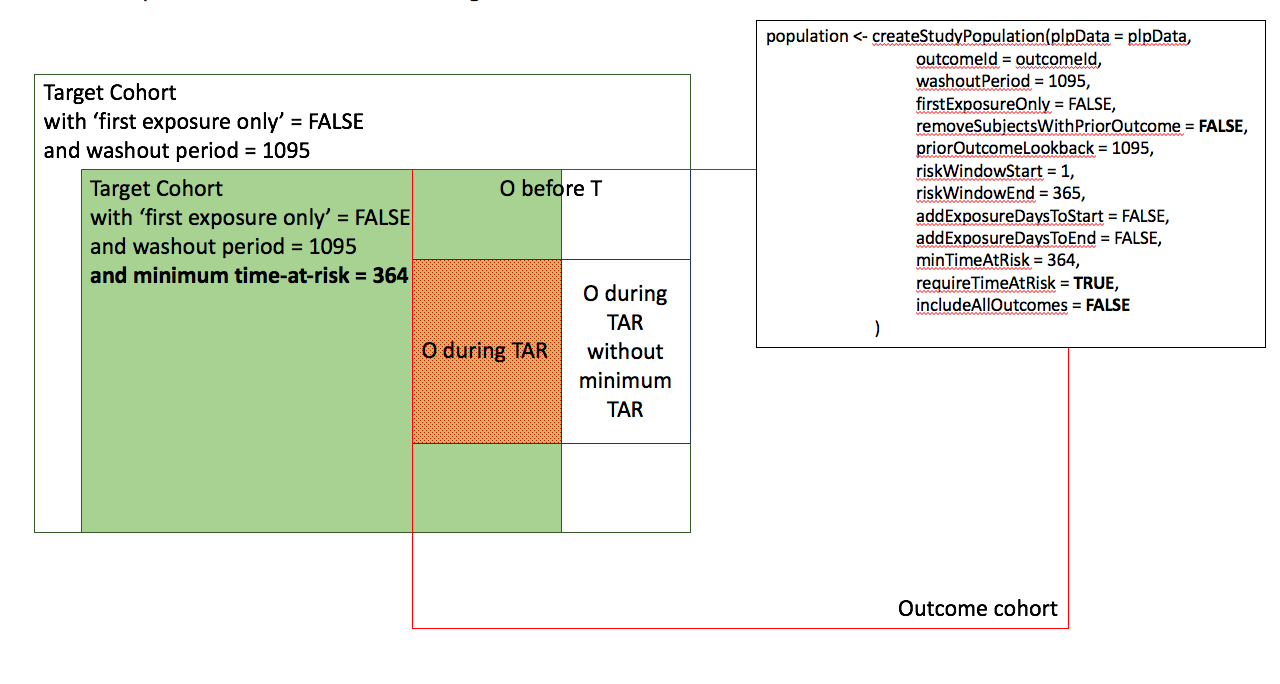
\includegraphics{popdef1.png}
\item
  Require minumum time-at-risk for target cohort, except for persons
  with outcomes during time-at-risk.

  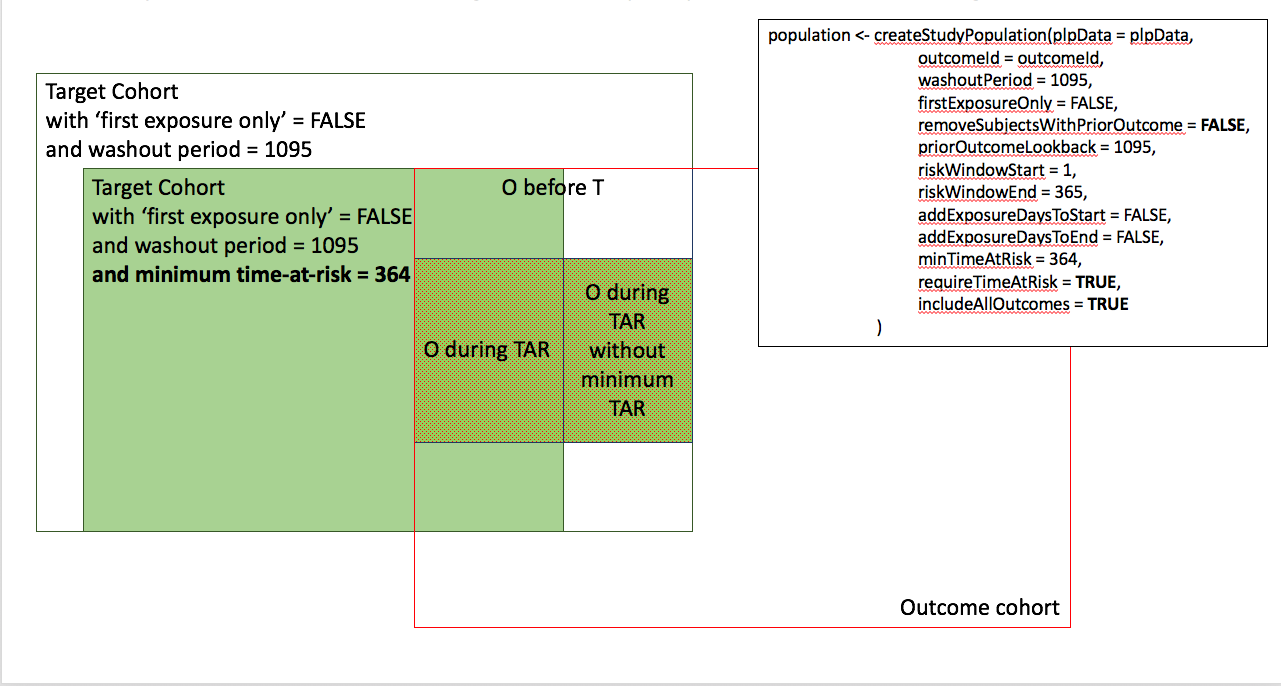
\includegraphics{popdef2.png}
\end{enumerate}

\newpage 3)

Include all persons in the target cohort exclude persons with prior
outcomes

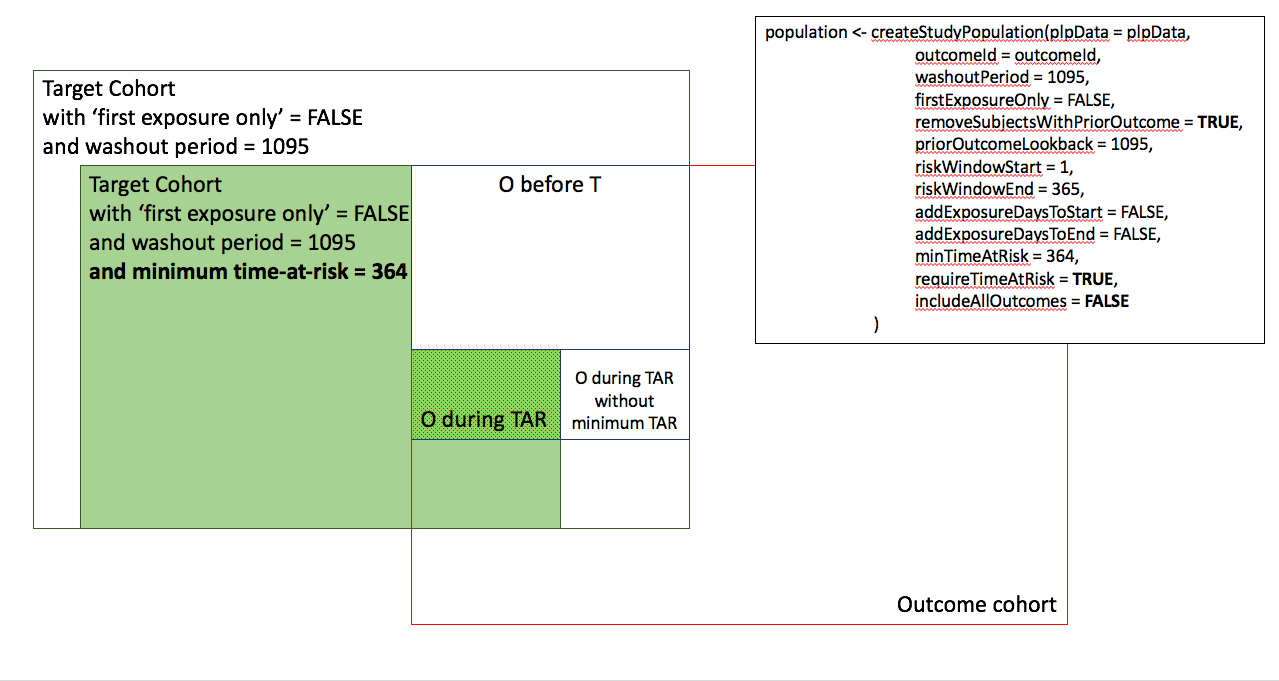
\includegraphics{popdef3.png}

\begin{enumerate}
\def\labelenumi{\arabic{enumi})}
\setcounter{enumi}{3}
\item
  Require minimum time-at-risk for target cohort, except for persons
  with outcomes during time-at-risk, exclude persons with prior outcomes

  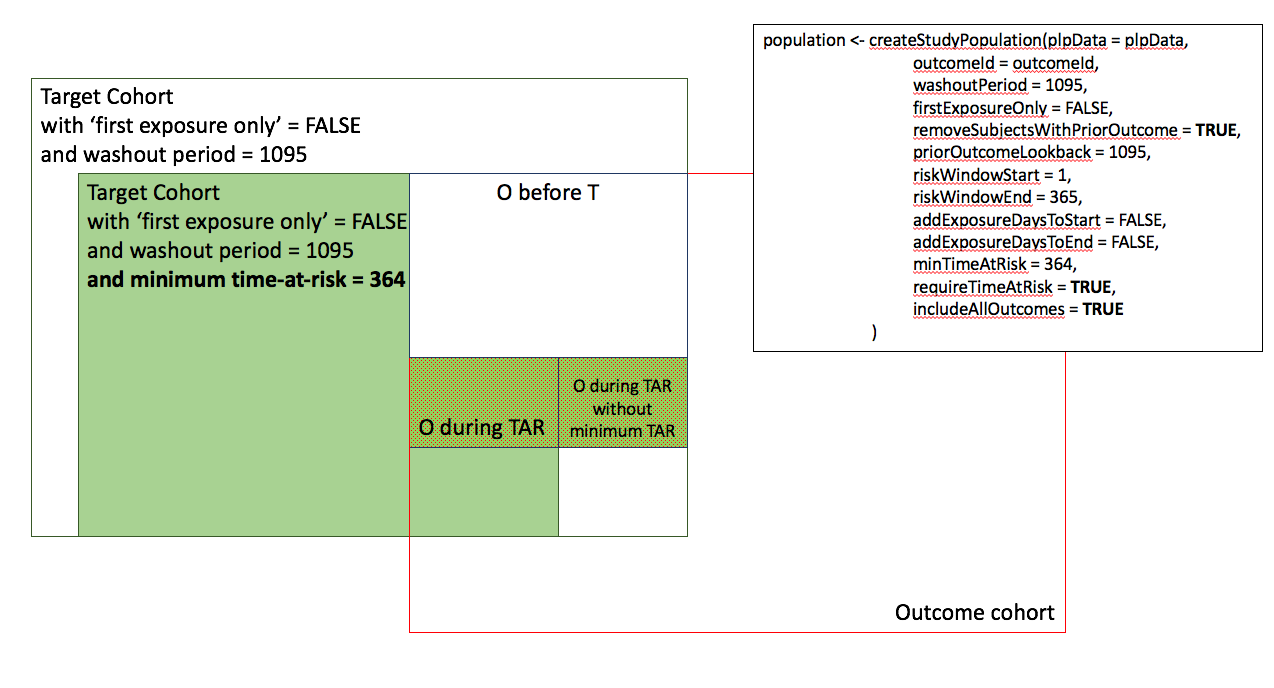
\includegraphics{popdef4.png}
\end{enumerate}

\newpage

\begin{enumerate}
\def\labelenumi{\arabic{enumi})}
\setcounter{enumi}{4}
\item
  Include all persons in target cohort exclude persons with prior
  outcomes

  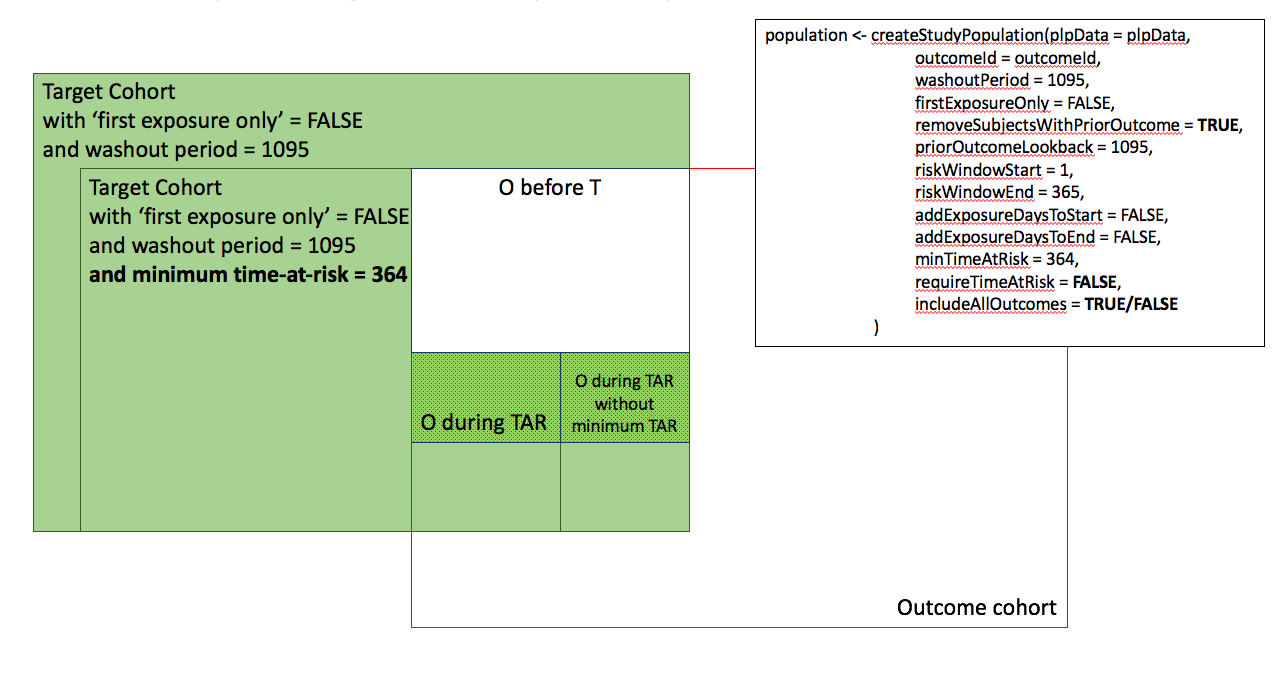
\includegraphics{popdef5.png}
\item
  Include all persons in target cohort

  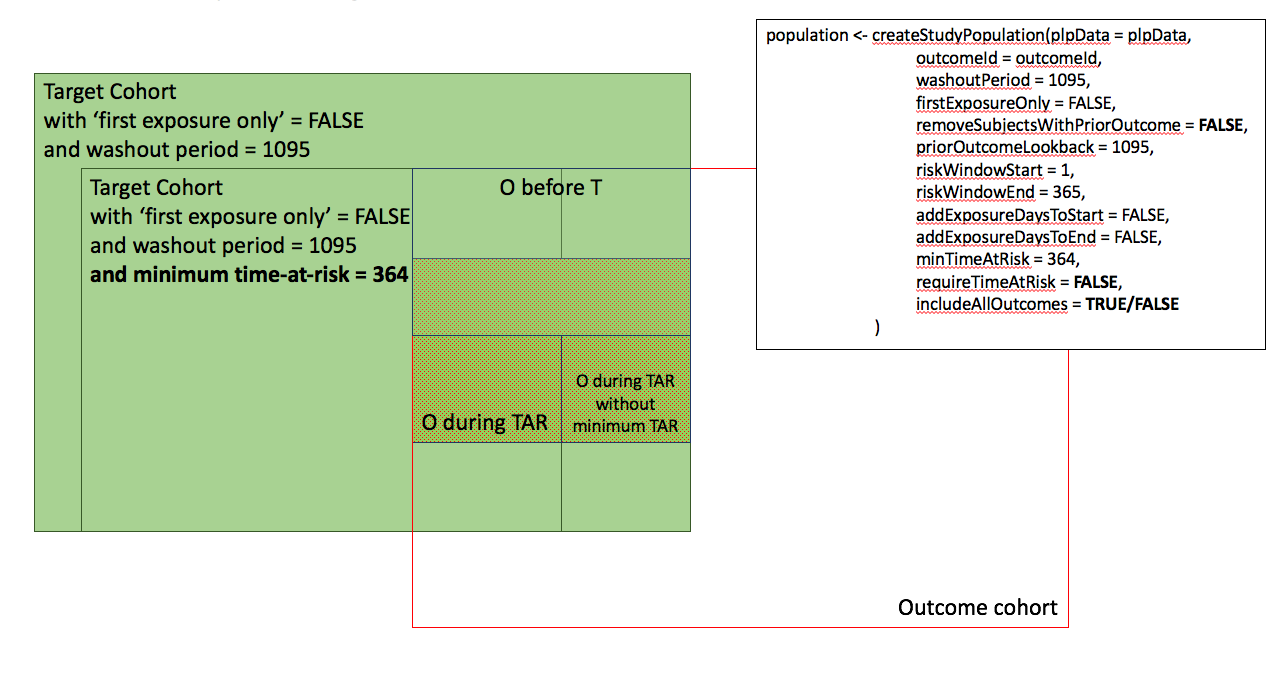
\includegraphics{popdef6.png}
\end{enumerate}

\end{document}
